\chapter{Simulation}
Two levels of simulation are discussed in this section. First the simulation of single time series
and second, a slice of simulated FMRI time series. The single time series tests
are necessary to investigate the power of particle filters in 
identifying the BOLD model in a noisy environment. If the particle filter is unable
to get back to the "true" time-series in spite of noise then the particle filter
will not be useful. Additionally, determination of reasonable parameters from the
time-series is also desirable. The reason to then simulate an entire slice is that
the "Possum" FMRI simulation tool models noise more realistically, for instance by
adding spatial correlation. Additionally 
it provides insight into the applicability of particle filters in modeling the BOLD 
signal on a large scale.

\section{Single Time Series}
Given the state-space equations for the BOLD signal, simulating a single time 
series is relatively straight forward. After a "true" signal is generated,
identically and independently distributed (I.I.D.) Gaussian noise and a Wiener
process with Gaussian I.I.D. steps are added to the true signal. Finally a 
"carrier level" is added, since BOLD is typically
measured as a \% difference from the baseline. The particle filter
algorithm will immediately remove this by calculating the \% difference, 
but adding a carrier level means that the exact same algorithm which 
will is used for simulated data may be used for the real data. 

Once this noisy simulated time series has been generated, the particle filter algorithm
 is then run on this single time series "image". Here I will include two sets of tests 
to determine the power of the particle filter in modeling. The first set are 
used to demonstrate the ability of the particle filter to find the most likely
set of parameters/state variables over the course of the run. The second type
of test will investigate the problem of false-positives. As the first
round of tests will show, given that there is an underlying BOLD signal, 
the particle filter is excellent at finding the most probable cause of 
the observed signal. However, as discussed in the false positive tests,
even if there is no true underlying signal, the particle filter will still determine
the most likely BOLD signal; which may not be flat. Thus, it is 
important to investigate methods of determining false positives using 
average residuals. This problem could in actuality never come up, for instance
if the number of measurements is very large or if the noise peaks are not
particularly large.

%LOW NOISE SECTION, with a signal
\subsection{Signal with Low Noise}
%tests had noise of $ \{\sigma_y = .01, \sigma_x = .005\} $, where $\sigma_y$ is the
%measurement noise, and $\sigma_x$ is the wiener step size. Both signals used the
%parameters .
%The particle filter used the parameters defined in \autoref{tab:Prior} (\autoref{sec:PriorDistrib}),
%thus the particle filter was not centered over the correct values. 
\begin{figure}
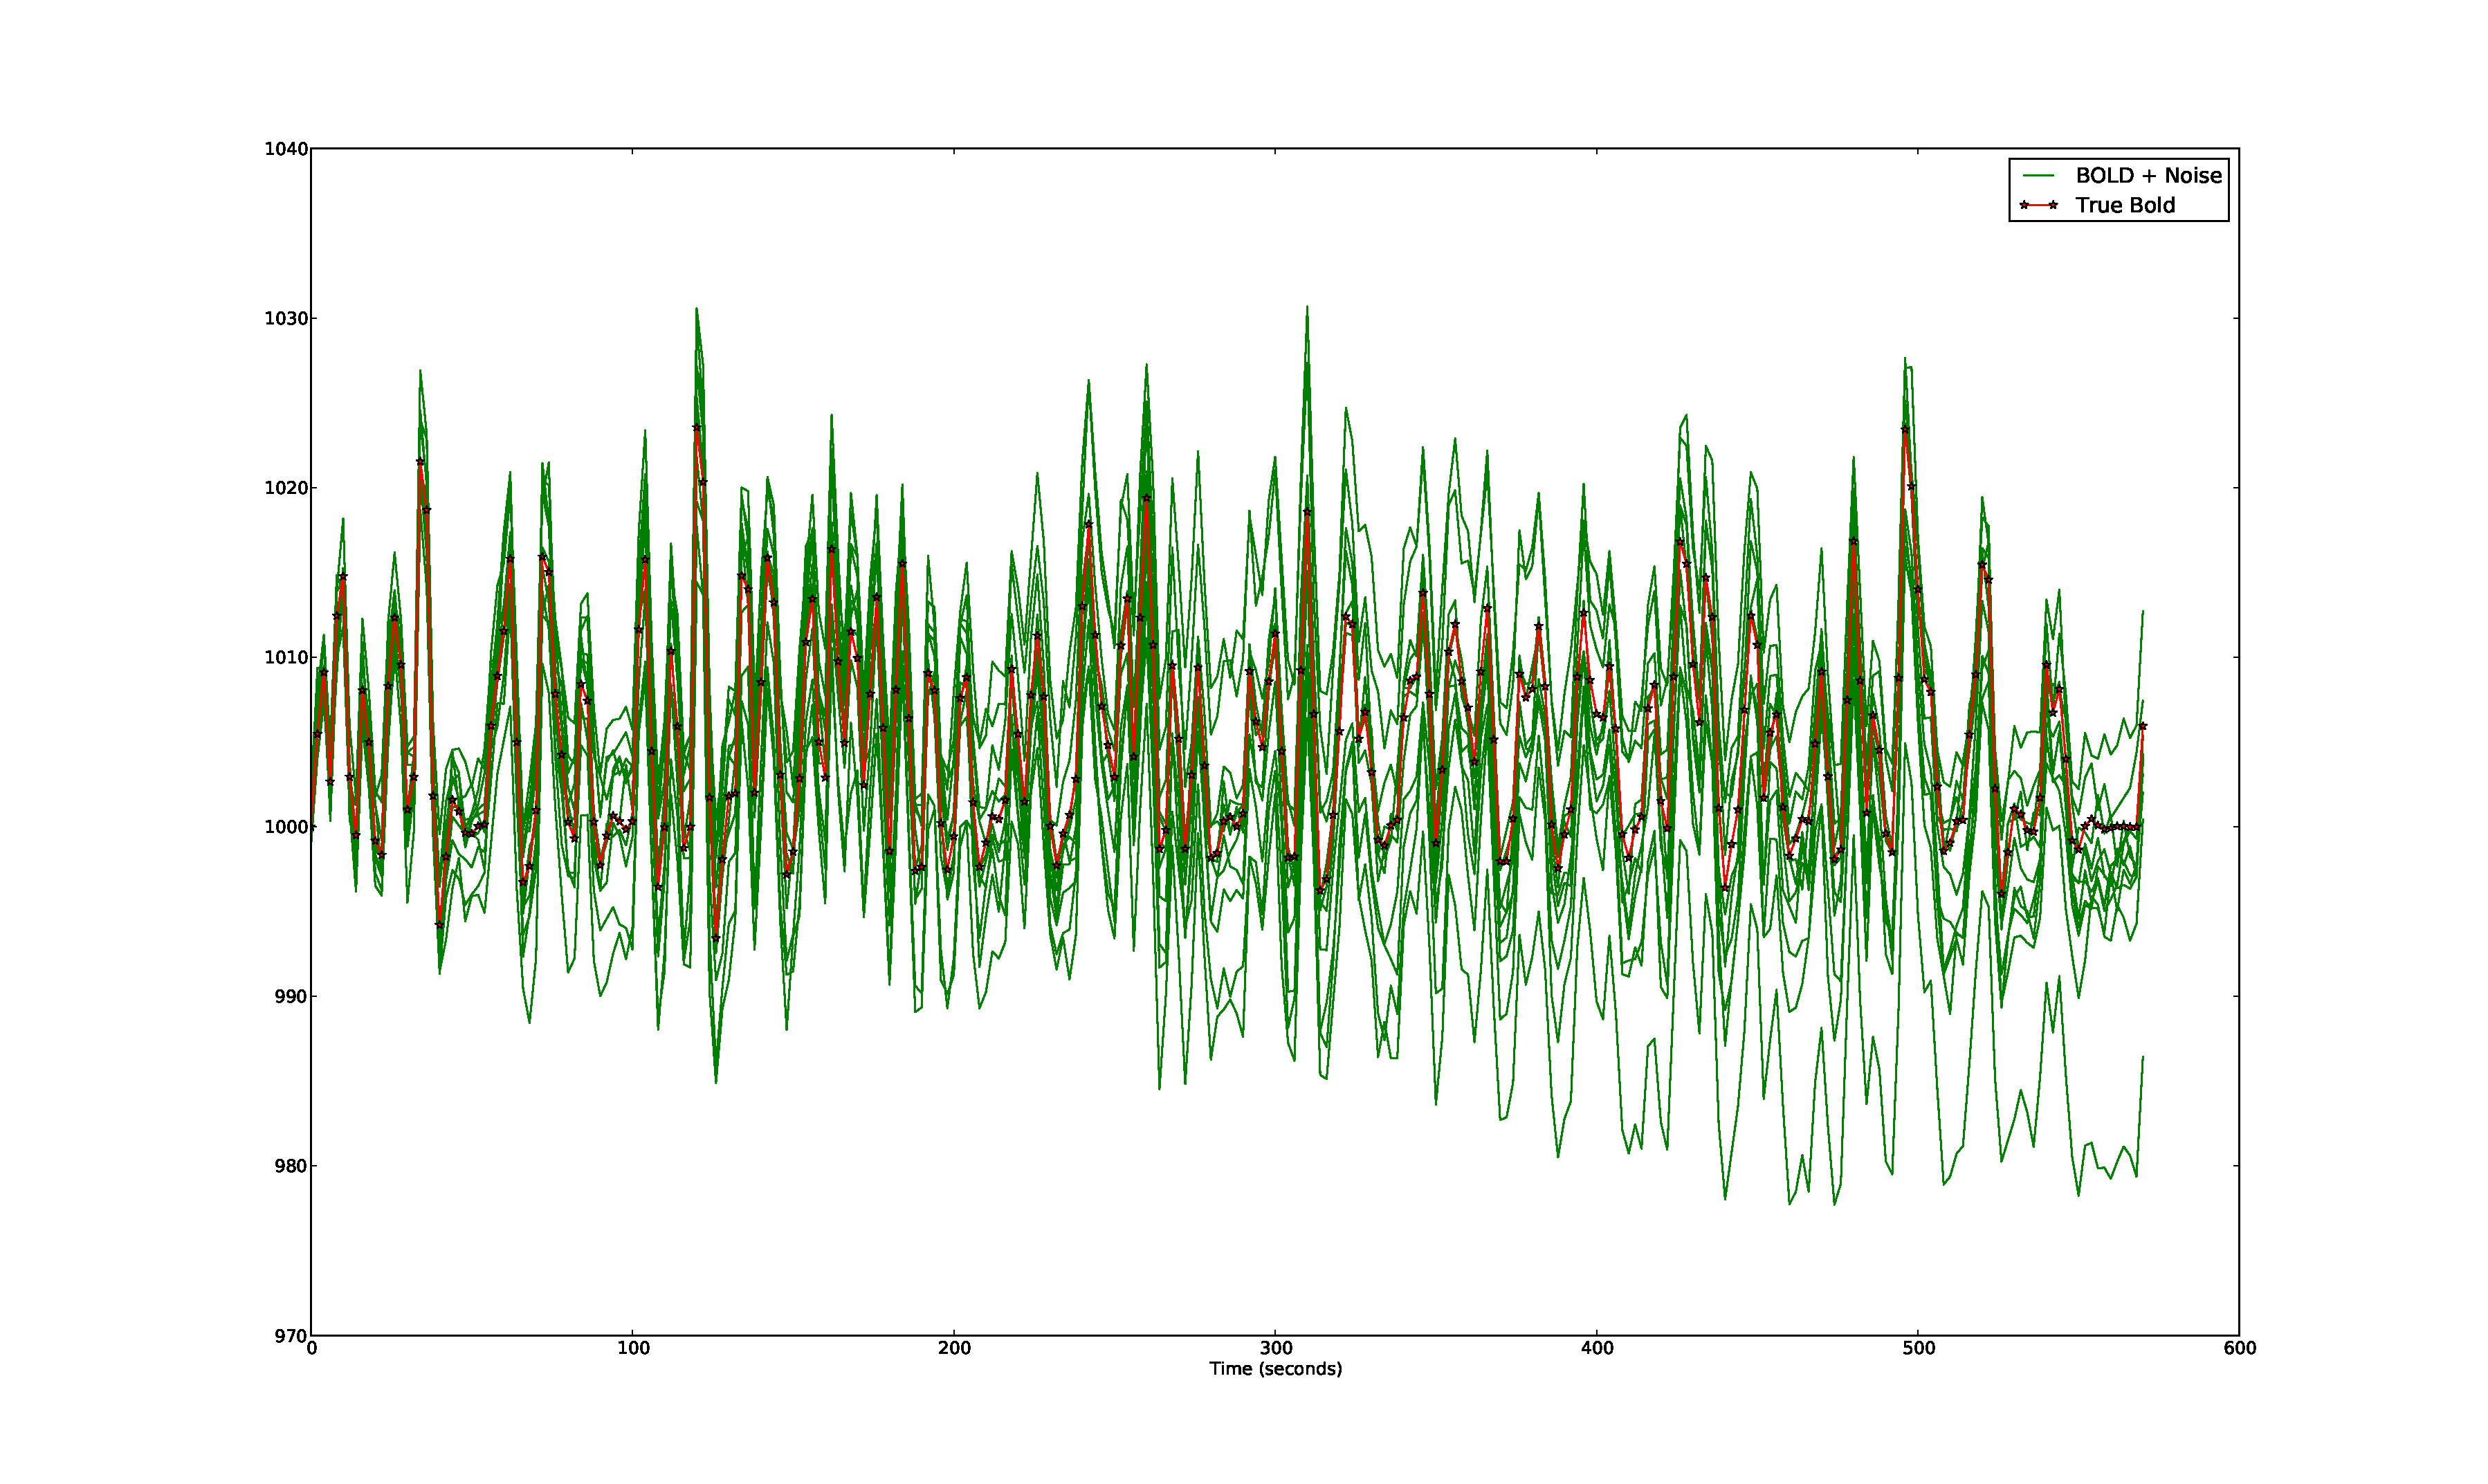
\includegraphics[clip=true,trim=6cm 2cm 6cm 3.5cm,width=17cm]{images/realization_lownoise}
\caption{Test Signals with low noise compared to the clean signal.}
\label{fig:LowNoiseRealization}
\end{figure}

\begin{figure}
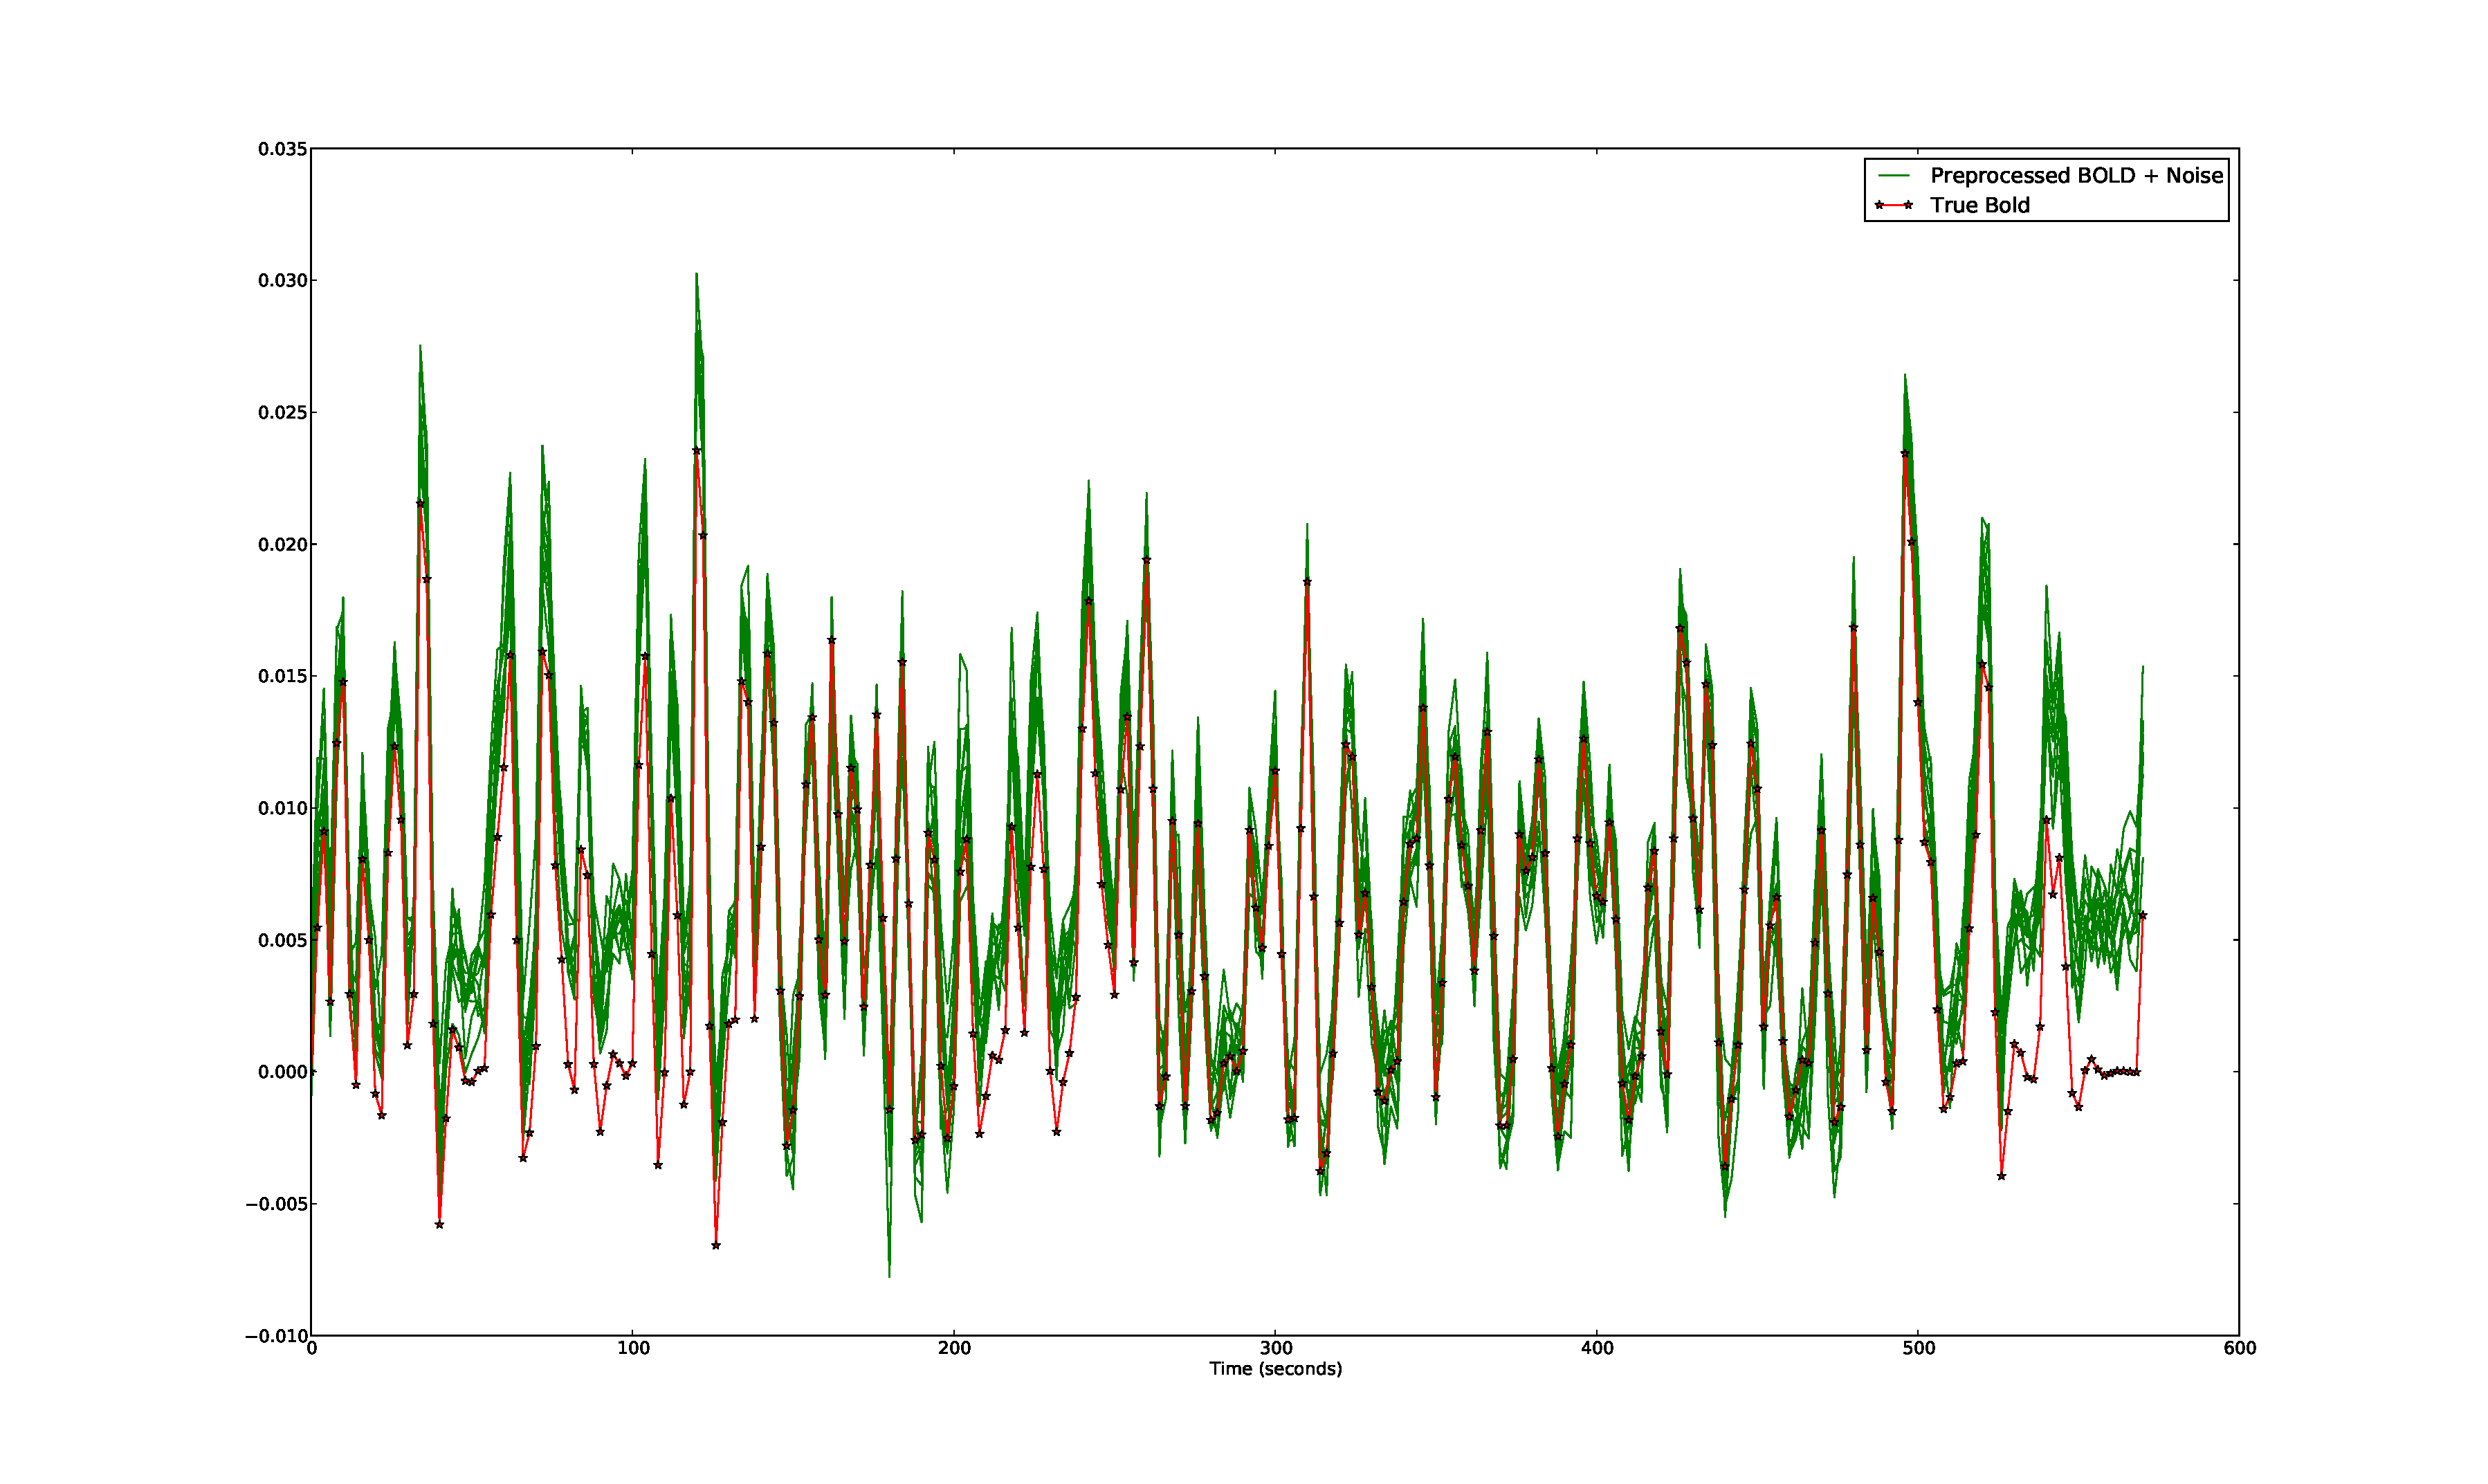
\includegraphics[clip=true,trim=6cm 2cm 6cm 3.5cm,width=17cm]{images/preprocessed_lownoise}
\caption{A comparison of the preprocessed signals for the low noise case. This is the
noisy input to the actual particle filter algorithm.}
\label{fig:PreprocessedLowNoise}
\end{figure}

\begin{figure}
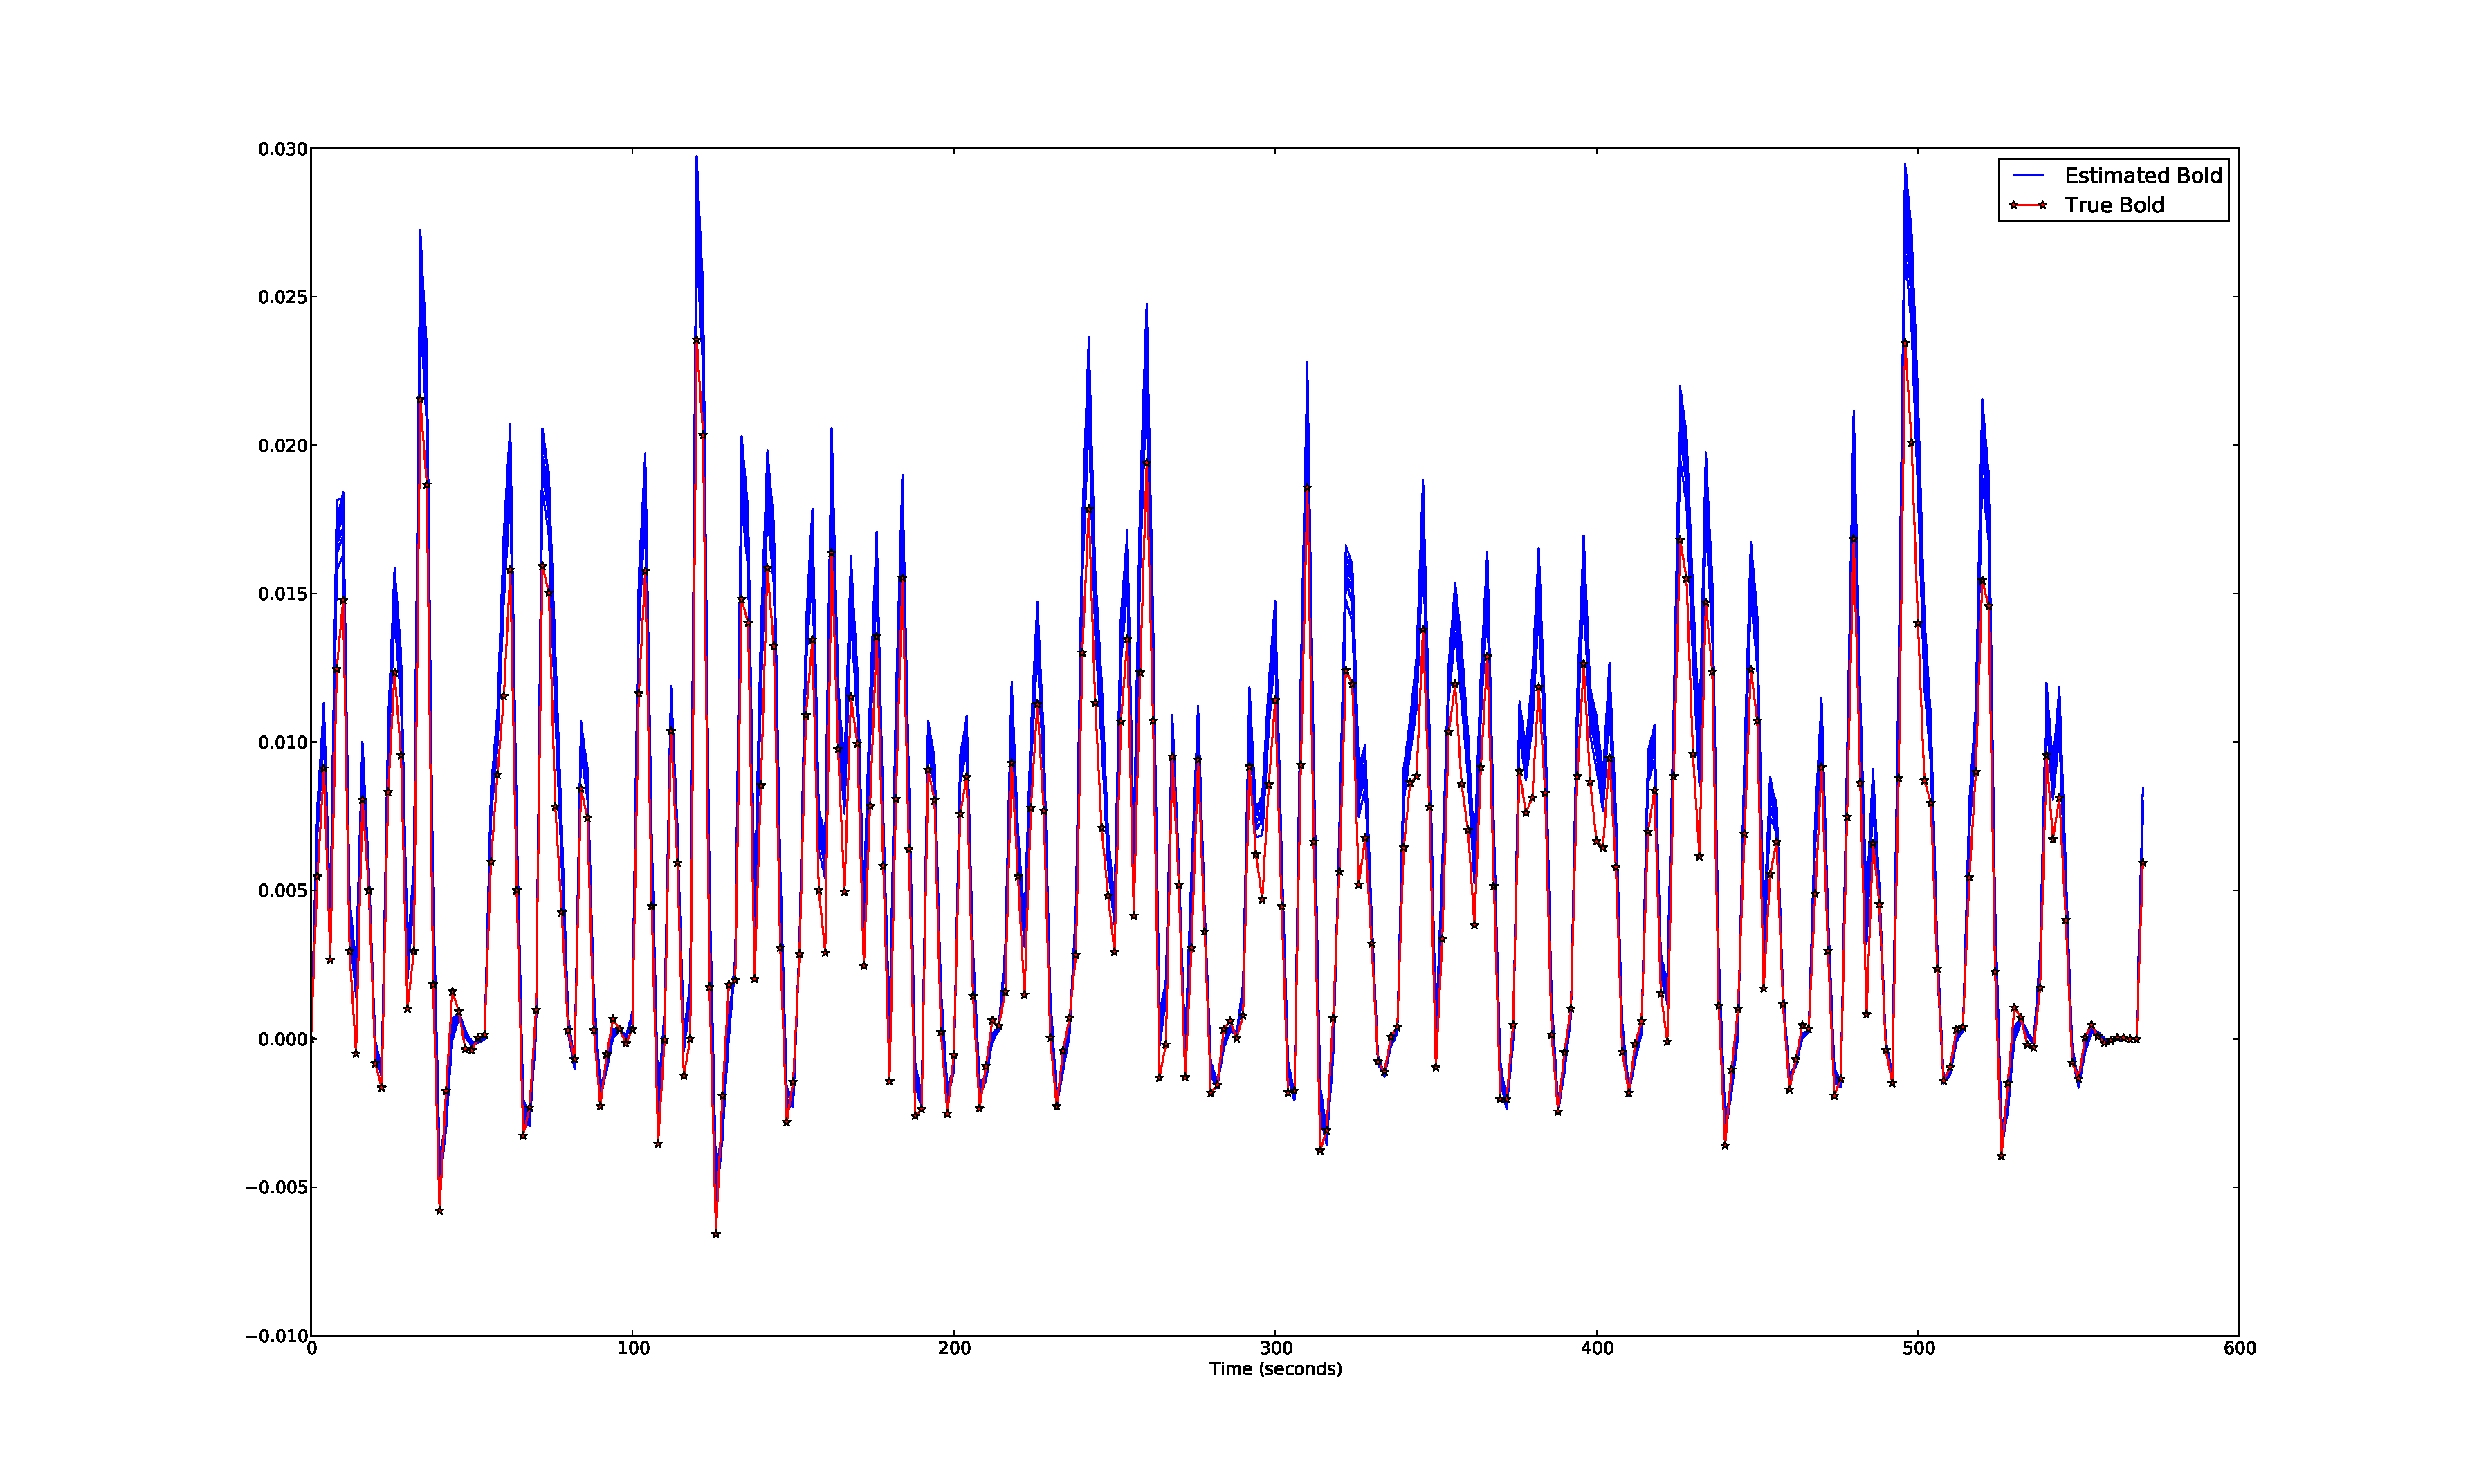
\includegraphics[clip=true,trim=6cm 2cm 6cm 3.5cm,width=17cm]{images/comparison_lownoise}
\caption{A comparison of the fitted signals for the low noise case.}
\label{fig:FitComparisonLowNoise}
\end{figure}

To begin the single voxel simulation; I generated a signal using the following parameters:
$\{\tau_0 = 1.45, \alpha = .3, E_0 = .47, V_0 = .044, \tau_s = 1.94, \tau_f = 1.99, \epsilon = 1.8\}$.
These same parameters will be used again in the high noise case. The noise realizations were
then based on a measurement noise, $\sigma_y$, of $.001$ and a drift standard deviation,
$\sigma_x$ of $.0005$. The measurement noise as well as the steps of the drift
were taken to be Gaussian
For this low noise case, the eleven realizations are shown in \autoref{fig:LowNoiseRealization}.
The actual signal that was delivered into the particle filter
is the result of some preprocessing to remove drift, as described in 
\autoref{sec:Methods Preprocessing}. The bias introduced into the signal by preprocessing 
may have some effect on the resulting fit; thus the preprocessed signal is compared
to the true BOLD signal in \autoref{fig:PreprocessedLowNoise}.
The preprocessing consists of several steps, which are discussed in detail in \autoref{sec:Methods Preprocessing}.
Obviously the spline struggles to match the signal near the end, as the graph shows, although 
overall, the preprocessing seems to have been successful at removing trends. Finally, the 
set of fits to the true BOLD signal are shown in \autoref{fig:FitComparisonLowNoise}.
The filtering property of the particle filter is clear from the results here.  In several locations the output
of the particle filter looks like a filtered version of the input. For instance toward the
end, the estimates stay flat in spite of the preprocessed data drifting off. By
this point, the algorithm has converged sufficiently to know that that such a movement in
signal isn't possible. A similar circumstance occurs at 100 seconds in. 
In general the fits are good, although the bias introduced by pre-processing clearly
results in a slightly larger peak signal. The final parameter sets are shown in 
\autoref{tab:LowNoiseResults}.

\begin{table}[t]
\centering
\begin{tabular}{|c | c | c | c | c | c | c | c | c | c |}
\hline 
$\tau_0$ & $\alpha$ & $E_0$    & $V_0$    & $\tau_s$ & $\tau_f$ & $\epsilon$  & $ \sum \tau $ & $\sqrt{MSR}$ &$\sqrt{MSE}$\\
\hline 
\rowcolor[gray]{.8}
1.45 & .3 & .47 & .044 & 1.94 & 1.99 & 1.8  & 5.38 &  & \\
\hline 
\hline 
1.2221 & 0.3449 & 0.3346 & 0.0714 & 1.6045 & 2.2753 & 1.5945 & 5.1019 &  0.003211  & 0.009876  \\
1.3749 & 0.3318 & 0.3630 & 0.0733 & 1.6408 & 2.1030 & 1.5763 & 5.1187 &  0.003055  & 0.009932  \\
1.1660 & 0.3221 & 0.3406 & 0.0822 & 1.6477 & 2.3535 & 1.2452 & 5.1672 &  0.003289  & 0.009680  \\
1.2318 & 0.3271 & 0.3403 & 0.0796 & 1.6270 & 2.1852 & 1.3033 & 5.0439 &  0.002847  & 0.009120  \\
1.1832 & 0.3179 & 0.3472 & 0.0821 & 1.5496 & 2.2912 & 1.2782 & 5.0240 &  0.003006  & 0.009713  \\
1.1424 & 0.334  & 0.3473 & 0.0737 & 1.6221 & 2.2908 & 1.4025 & 5.0553 &  0.002833  & 0.009485  \\
1.3004 & 0.3596 & 0.3564 & 0.0768 & 1.5641 & 2.1323 & 1.6034 & 4.9968 &  0.003028  & 0.010219  \\
1.2401 & 0.3460 & 0.3398 & 0.0891 & 1.6499 & 2.2366 & 1.2900 & 5.1265 &  0.003044  & 0.010080  \\
1.1709 & 0.3274 & 0.3464 & 0.0826 & 1.5373 & 2.2826 & 1.3783 & 4.9909 &  0.003345  & 0.010329  \\
1.1897 & 0.3434 & 0.3355 & 0.0798 & 1.5358 & 2.3075 & 1.4277 & 5.0330 &  0.003175  & 0.010015  \\
1.184 &  0.3405 & 0.3502 & 0.0892 & 1.6103 & 2.2793 & 1.1645 & 5.0735 &  0.002889  & 0.009505  \\
\hline                                                                           
1.2187 & 0.3359 & 0.3456 & 0.0800 & 1.599 & 2.2488 & 1.3876 & 5.0665 & 0.003066     & 0.009814 \\
\hline 
\end{tabular}
\caption{Estimated Parameters on 11 different runs with low noise. First row is the true parameters,
last is mean over the 11 runs. The $\sqrt{MSR}$ is the square root of the mean square of the
residuals. Although in real data I won't distinguish between residual and error, here I will.
$\sqrt{MSE}$ is the mean squared difference between the true signal and the estimated signal.
This is the actual error, due to a combination of noise and preprocessing. }
\label{tab:LowNoiseResults} 
\end{table}

\begin{table}[t]
\centering
\begin{tabular}{|c | c  c  c  c  c  c  c |}
\hline 
  & $\tau_0$ & $\alpha$ & $E_0$    & $V_0$    & $\tau_s$ & $\tau_f$ & $\epsilon$ \\
\hline 
\rowcolor[gray]{.8} $\tau_0$ &   0.0189481 & -0.0014269 & -0.0011267 & -1.13e-05 & -0.0025616 & -0.0189559 & 0.0070405 \\
$\alpha$ &                       -0.0014269 & 0.0026716 & 9.93e-05 & -0.0002041 & -0.0008632 & -0.0016823 & 0.0071891 \\
\rowcolor[gray]{.8} $E_0$    &   -0.0011267 & 9.93e-05 & 0.0010701 & -0.0002277 & -0.0001177 & 0.0001013 & 0.0016972 \\
$V_0$    &                       -1.13e-05 & -0.0002041 & -0.0002277 & 0.0005401 & 4.3e-06 & 4.56e-05 & -0.0080494 \\
\rowcolor[gray]{.8} $\tau_s$ &   -0.0025616 & -0.0008632 & -0.0001177 & 4.3e-06 & 0.0128056 & 0.012878 & -0.005516 \\
$\tau_f$ &                       -0.0189559 & -0.0016823 & 0.0001013 & 4.56e-05 & 0.012878 & 0.0416927 & -0.0158182 \\
\rowcolor[gray]{.8} $\epsilon$&  0.0070405 & 0.0071891 & 0.0016972 & -0.0080494 & -0.005516 & -0.0158182 & 0.1567165 \\
\hline 
\end{tabular}
\caption{Typical Covariance matrix of the parameters at the end of a run.}
\label{tab:CovSim} 
\end{table}

\begin{figure}
\subfigure[Converging histogram for $\tau_0$, $\alpha$, $E_0$, and $V_0$ of the first run, low noise simulation.]
{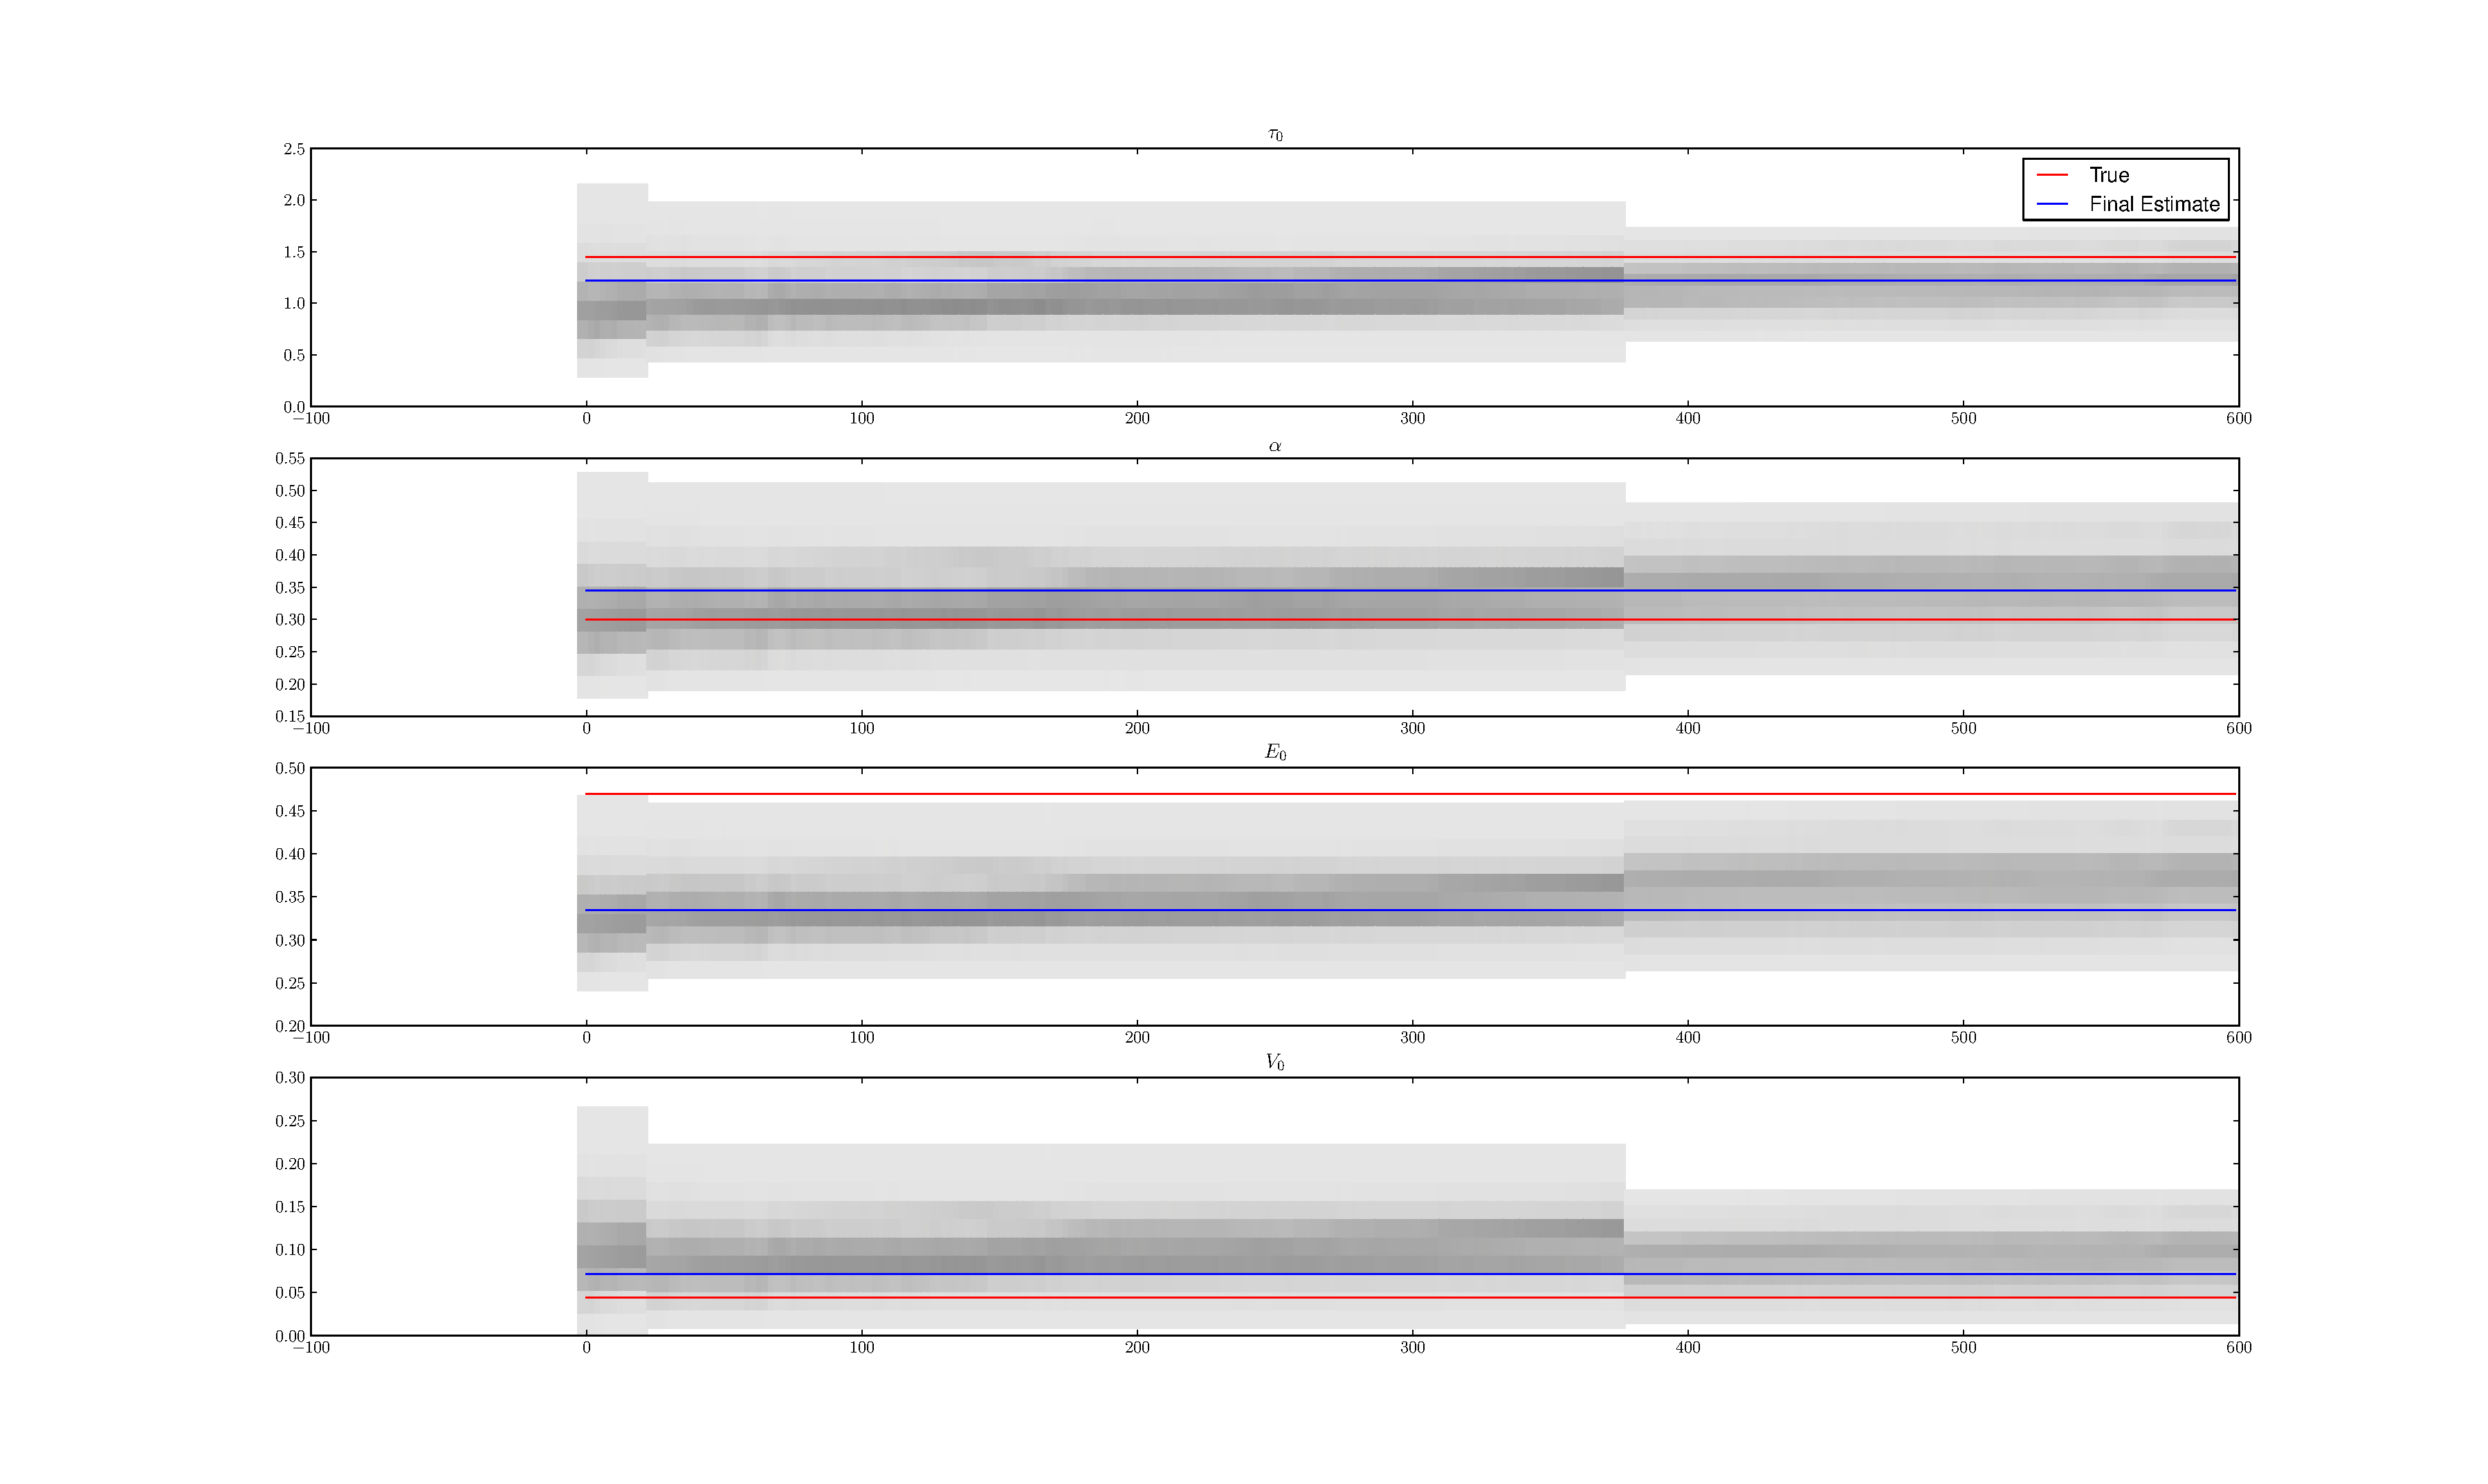
\includegraphics[clip=true,trim=7cm 3cm 6cm 3cm, width=16cm]{images/converge_lownoise1}}\\

\subfigure[Converging histogram for $\tau_s$, $\tau_f$, $\epsilon$, and $V$ of the first run, low noise simulation.]
{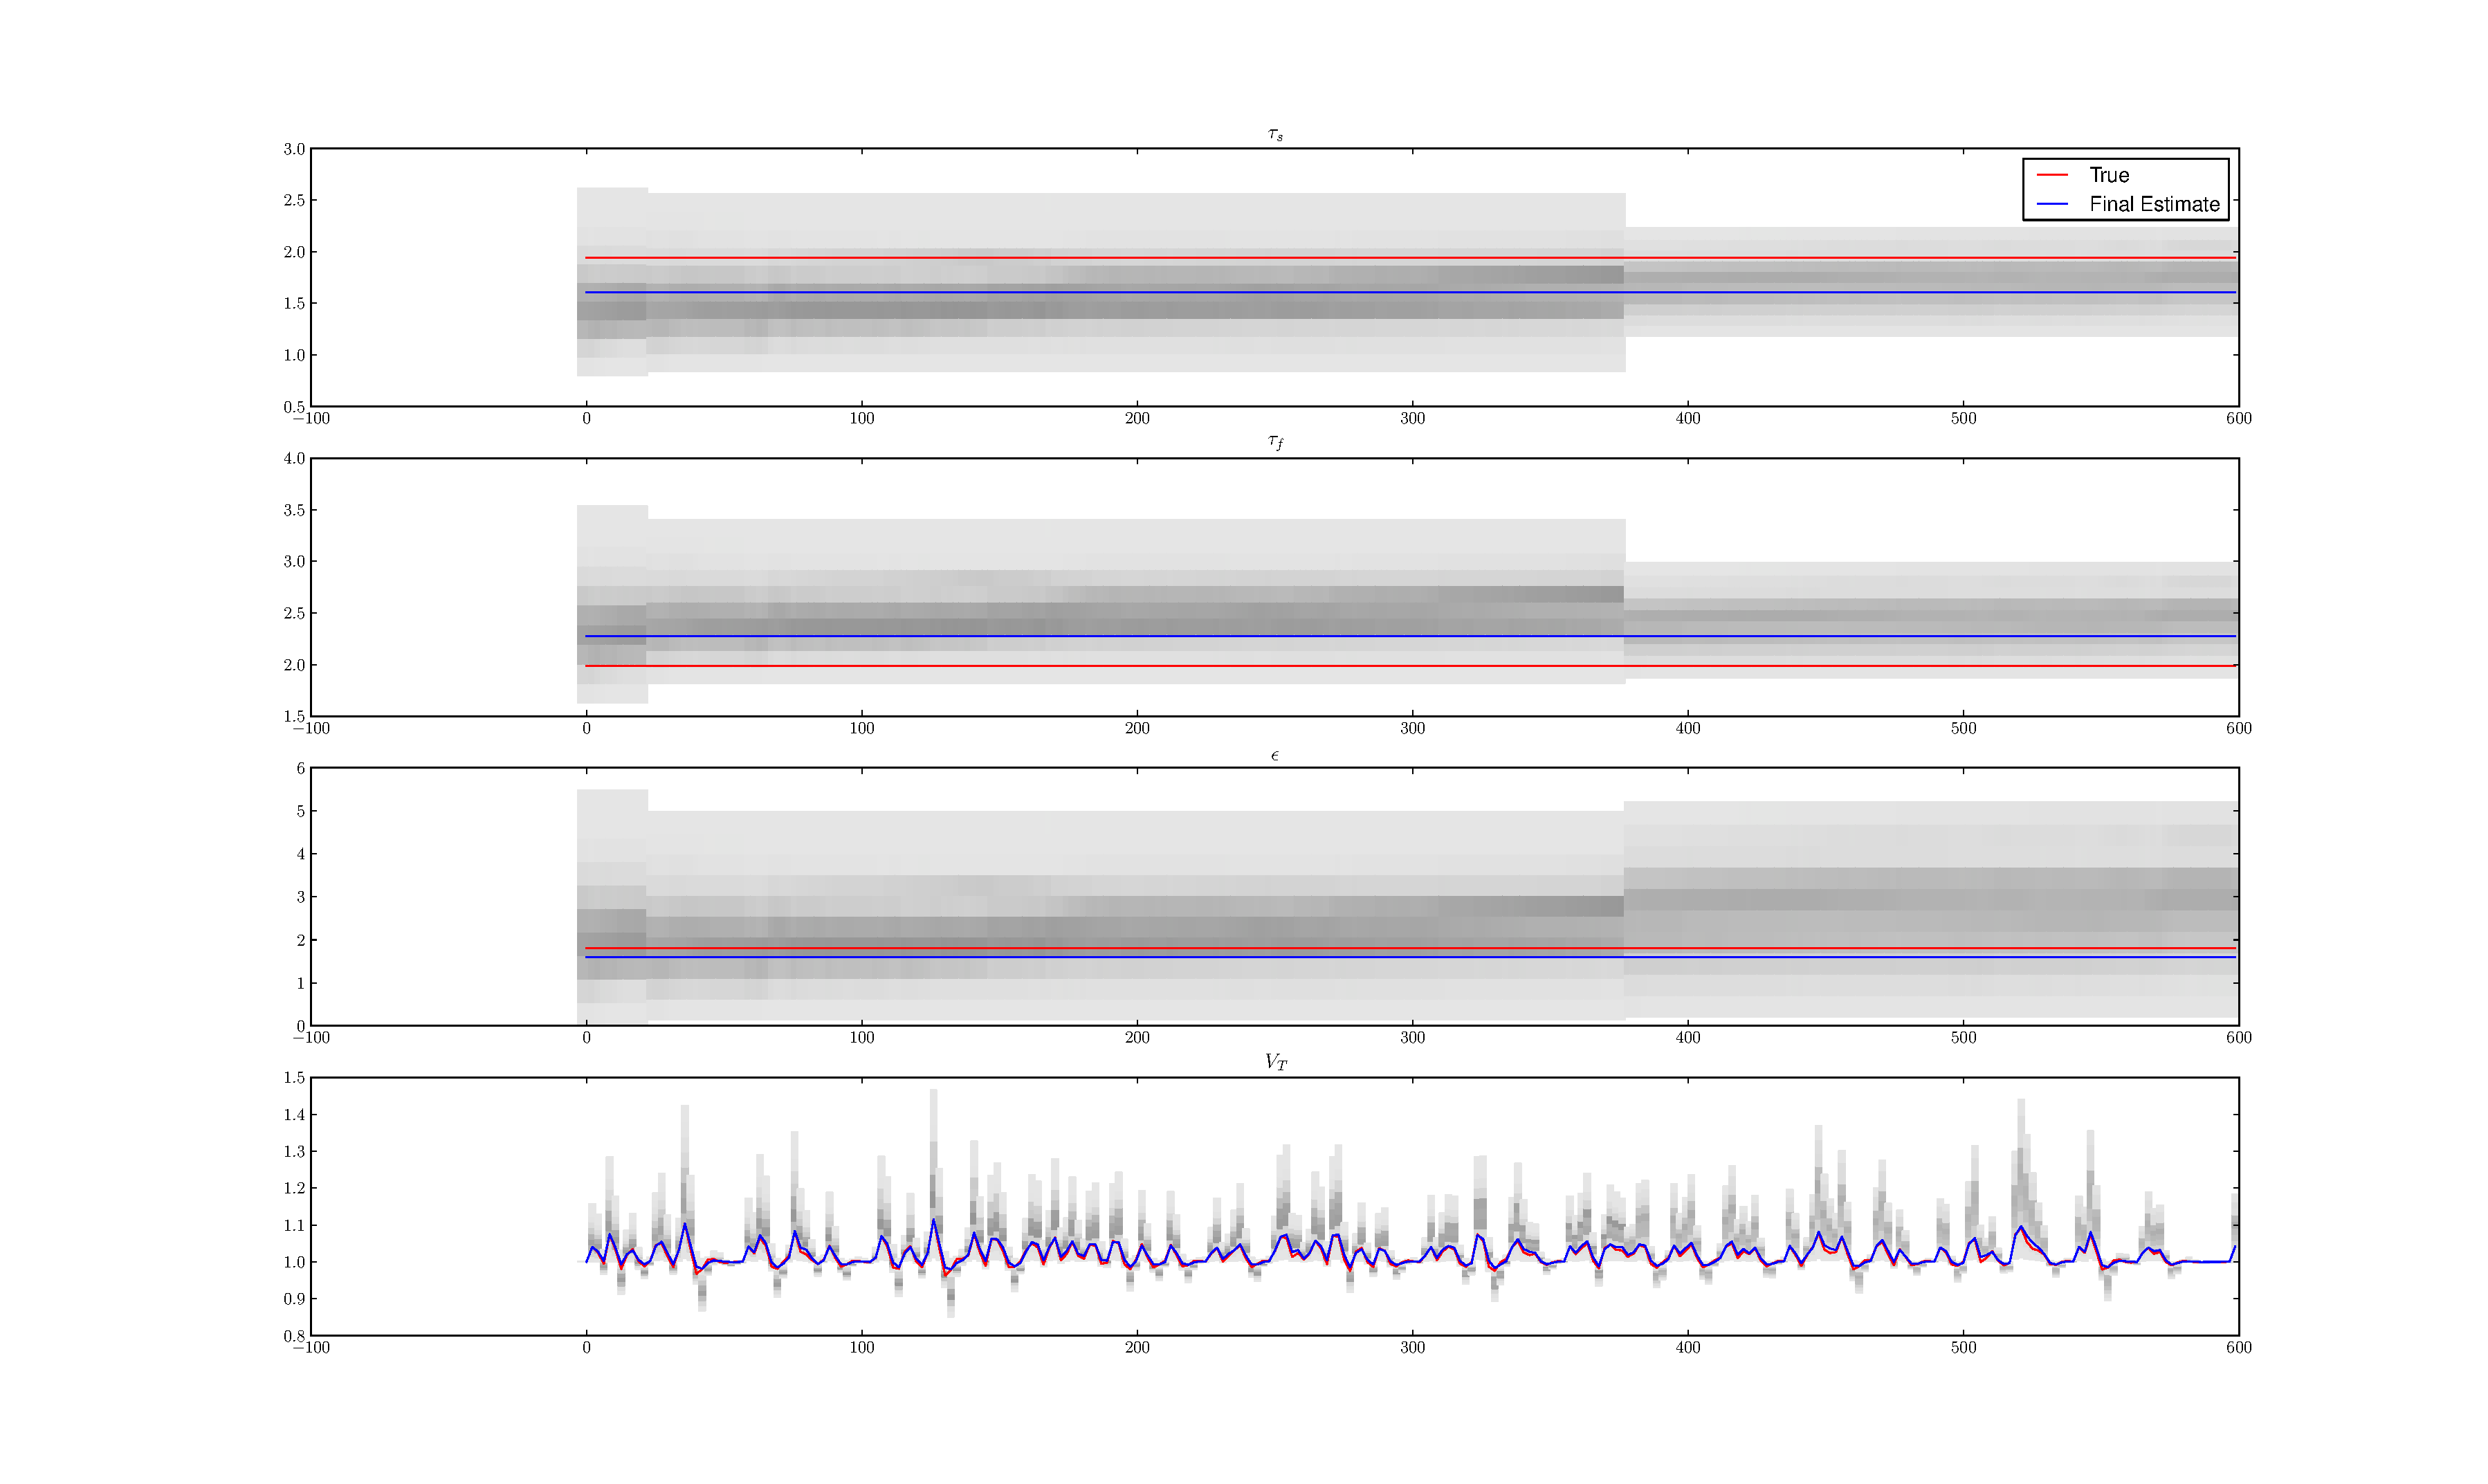
\includegraphics[clip=true,trim=7cm 3cm 6cm 3cm, width=16cm]{images/converge_lownoise2}}\\
\end{figure}

\begin{figure}
\subfigure[Converging histogram for $Q$, $S$, $F$, and $BOLD$ of the first run, low noise simulation.]
{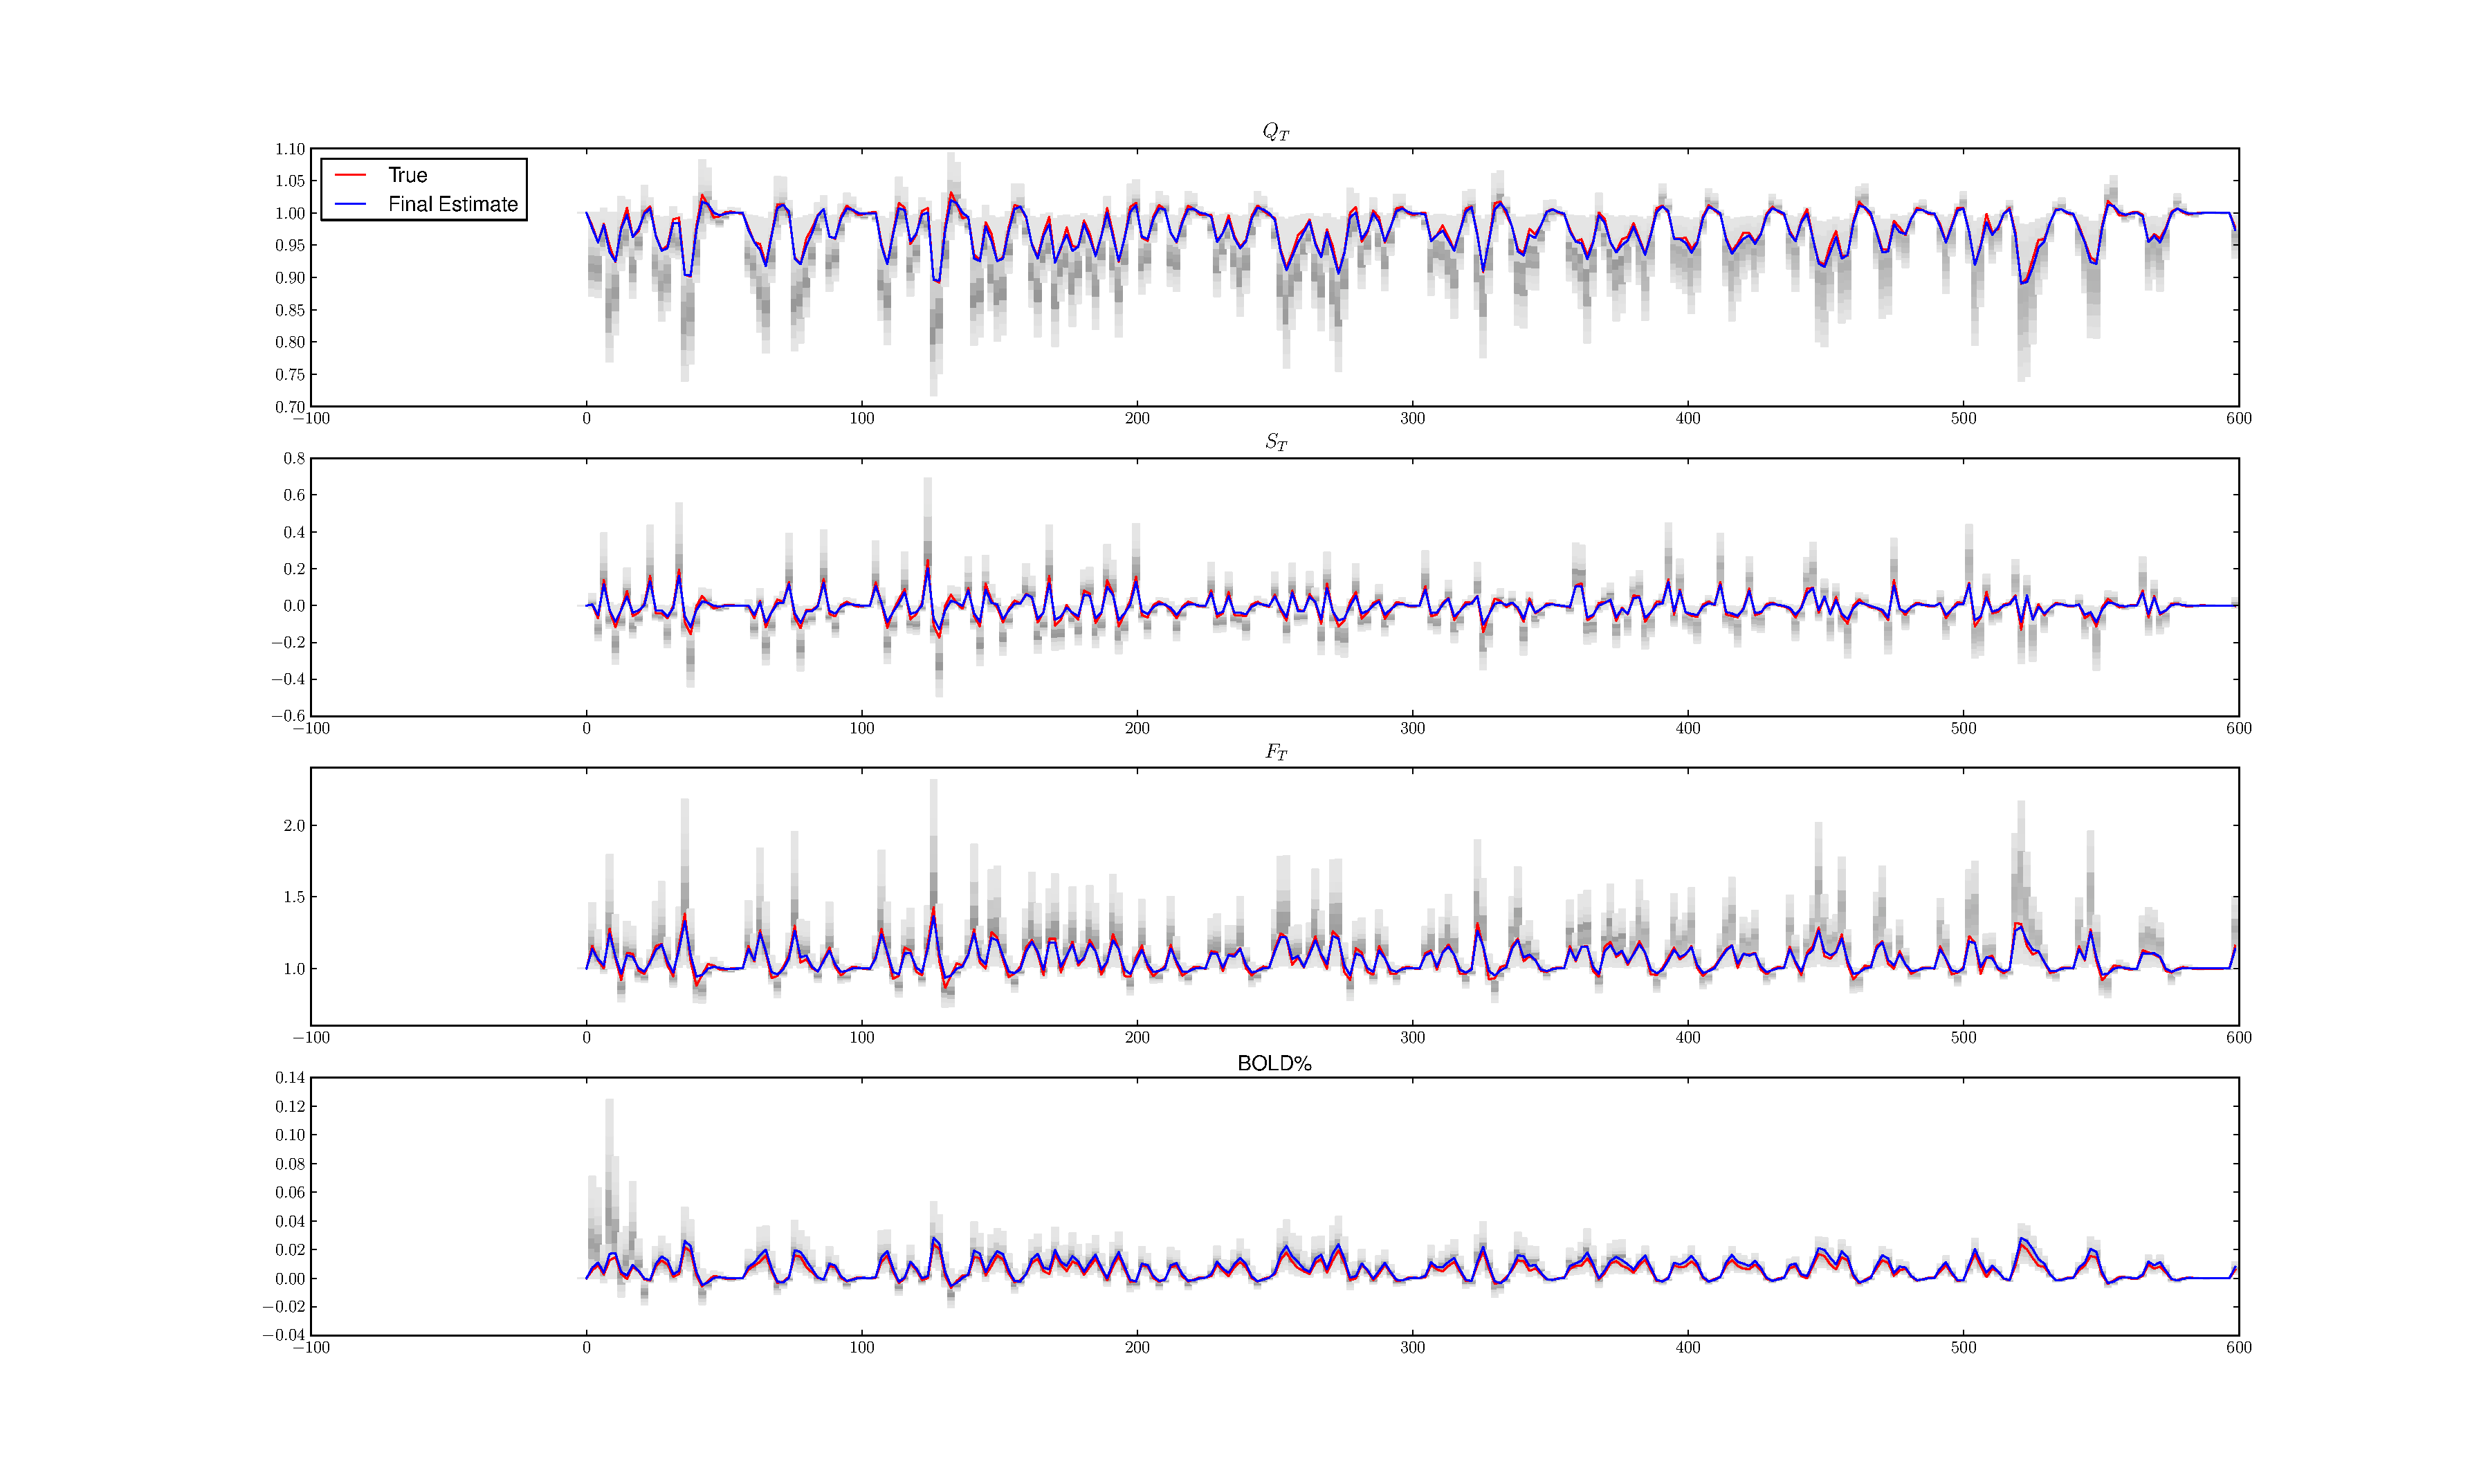
\includegraphics[clip=true,trim=7cm 3cm 6cm 3cm, width=16cm]{images/converge_lownoise3}}
\label{fig:LowNoiseHist}
\end{figure}

There are a few results worth noting here. First the time constants vary greatly across
runs with different noise realizations, yet the sum of the individual time constants
($\tau_f$, $\tau_s$ and $\tau_0$) seems to be more consistent. In general the 
time constants are falling short of the true time constant. This could be a limitation
based on the prior distribution (which notably has an initial mean below the true values) 
or it could be caused by the disassociated benefits of a correct time
constant with correct output. It often takes several measurement periods before a difference
in time constants becomes relevant to the weight. Its also possible that output is insensitive
to changes in the time constants and that varying the activation durations would 
cause the variations to be more visible. Another interesting result in the huge variation 
in the levels of $V_0$. In general,
with this admittedly small amount of noise, it would appear that the relation between a set
of parameters/stimuli and the output is not injective. In other words,  a time
series is not unique to a single set of parameters. This is good justification that 
simultaneous blood volume or tagged flow calculations with the conventional FMRI 
could benefit the model. 

The covariance matrix (\autoref{tab:CovSim}) also confirms the idea that the 
$\tau$ parameters are interchangeable
as far as the BOLD signal is concerned. Notice the covariance of $\tau_f$ and $\tau_0$
is $-0.019$ whereas
the variance of $\tau_0$ and $\tau_f$ are $0.019$ and $0.04$ respectively. Clearly there is 
some measure of ill-defined behavior between the different time-constants, as well as several
other variables.  The convergence properties of the first run in \autoref{tab:LowNoiseResults} 
demonstrates the migration of parameters to match the estimates. Given the relatively high
variance of parameters, its likely that more measurements or perhaps more variation
in the stimuli could further differentiate the parameters. Its also notable that
the final mean of the parameters may not be the best point estimator, and that perhaps
using the mode would be a better way to estimate the output. Regardless, the time series'
generated from the estimated mean seems to match the correct signal very well 
(\autoref{fig:FitComparisonLowNoise}).

%HIGH NOISE SECTION, with a signal
\subsection{High Noise}
\label{sec:HighNoise}
\begin{figure}
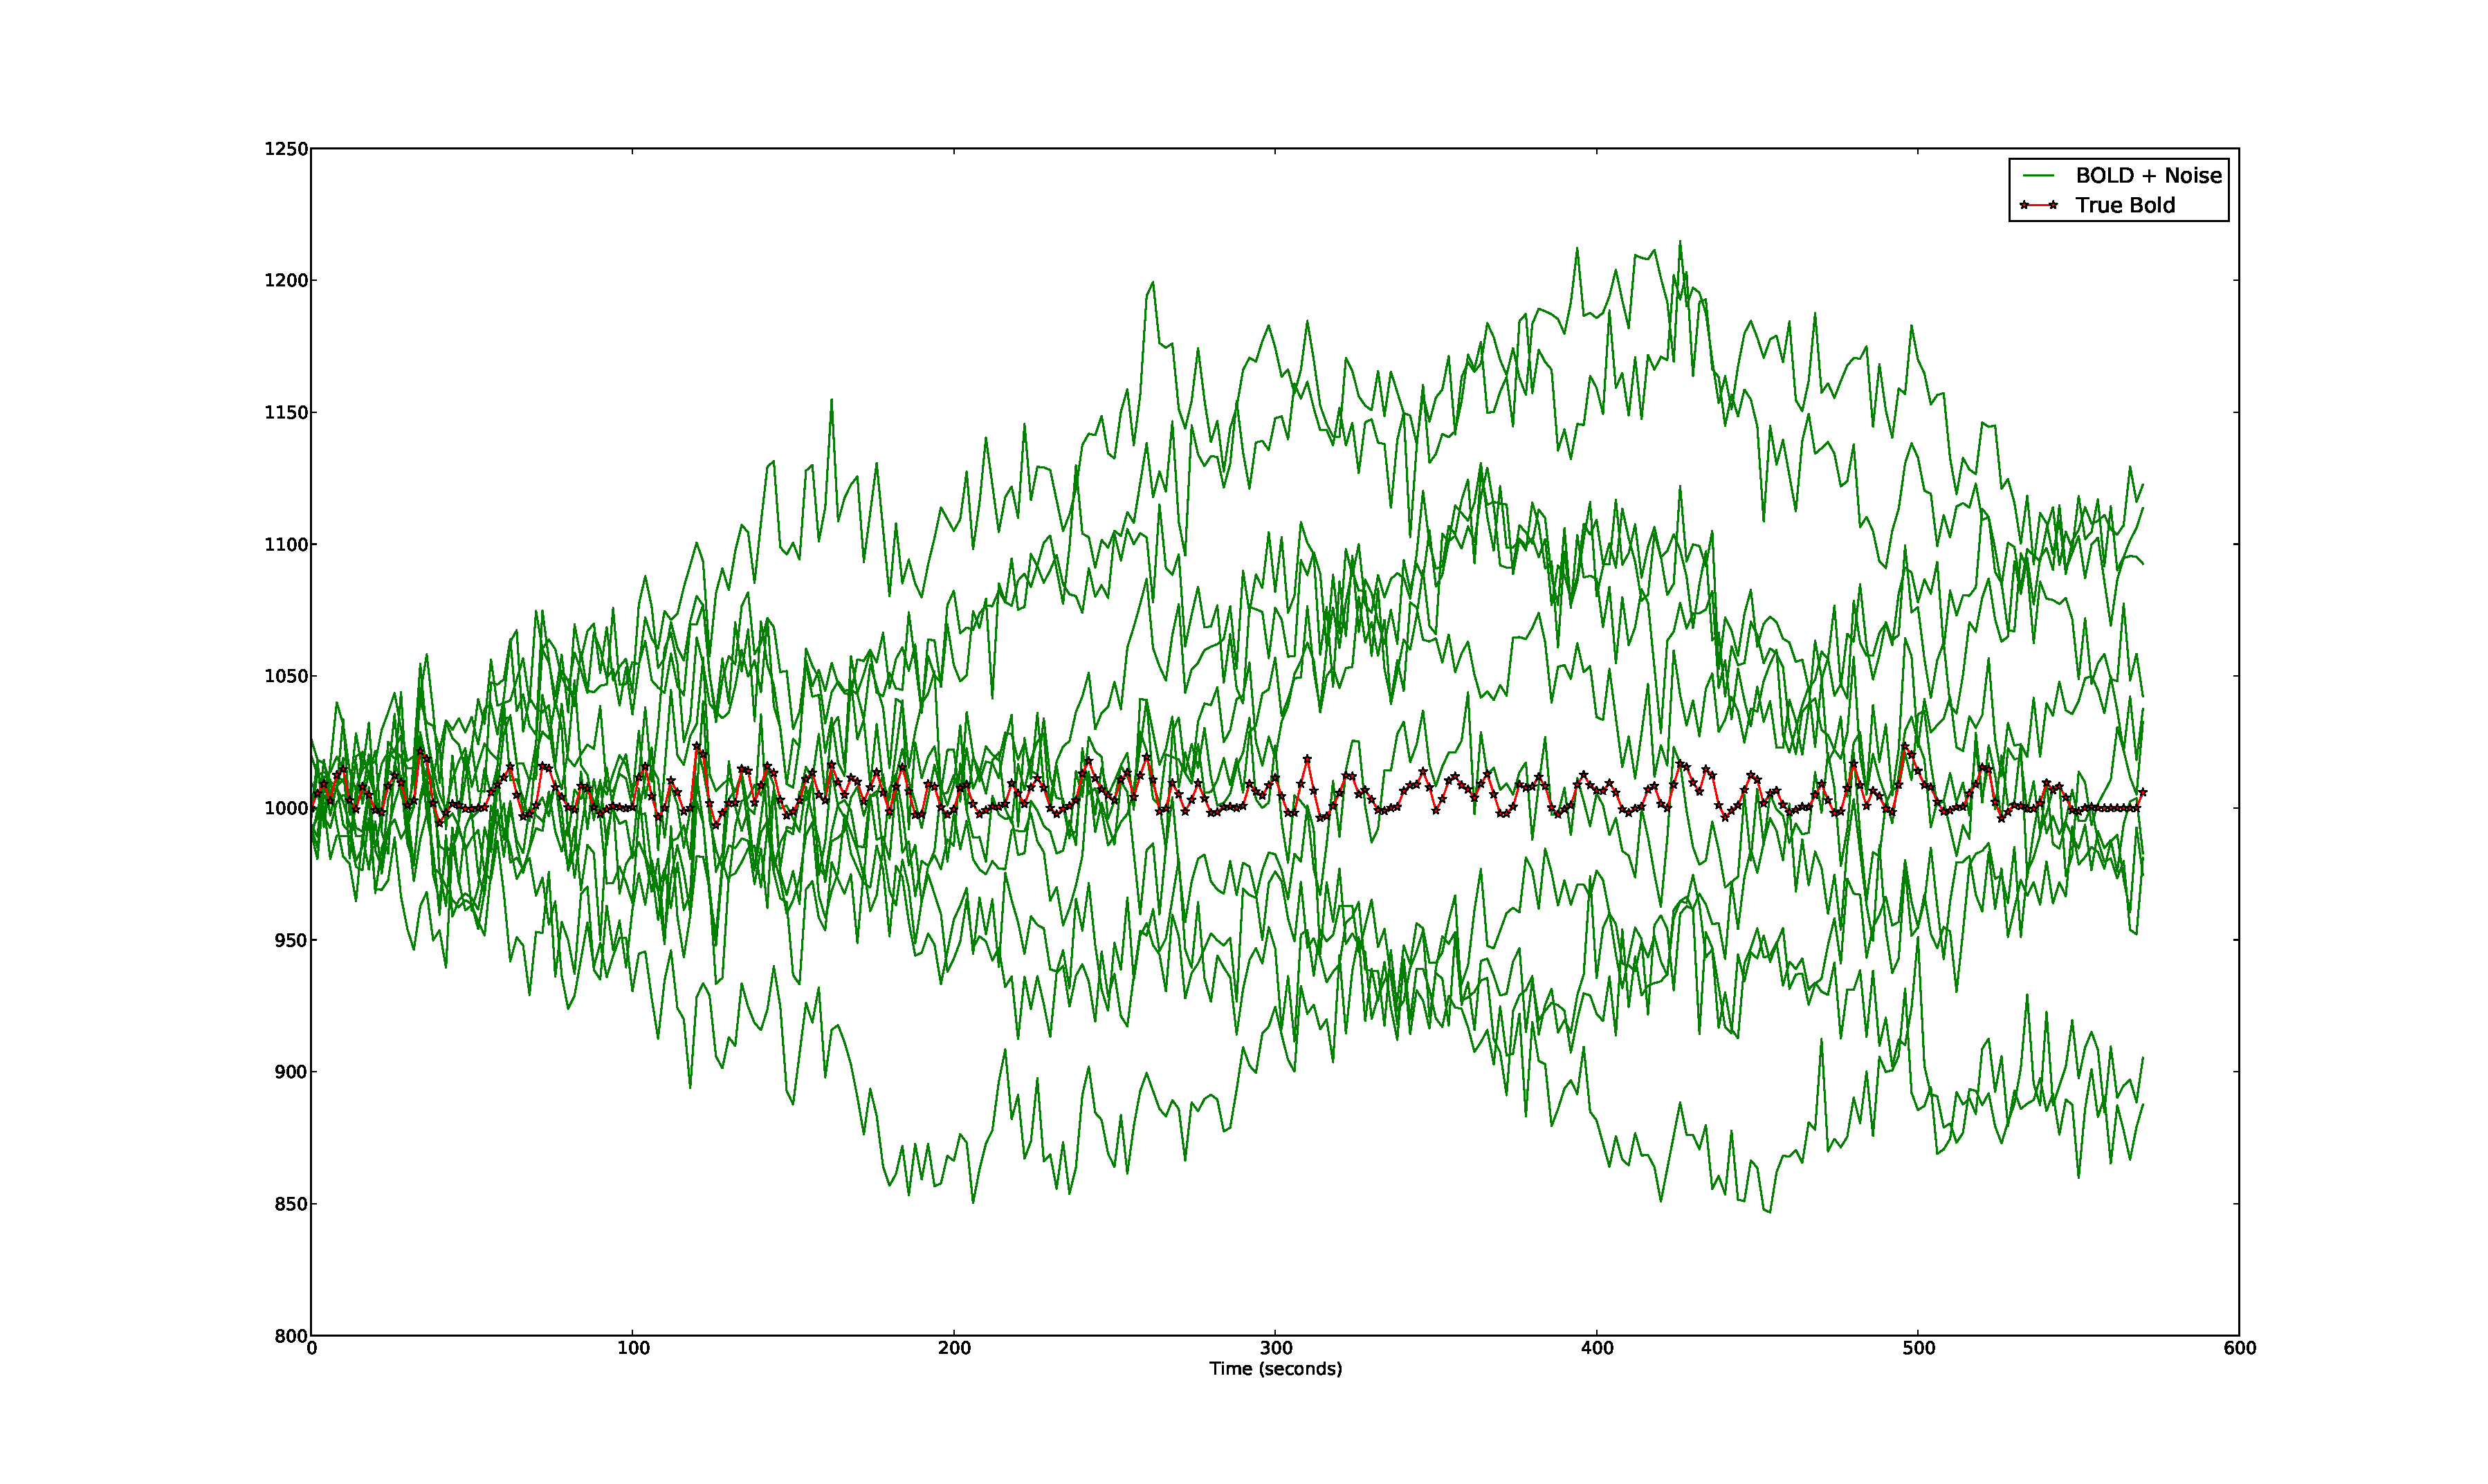
\includegraphics[clip=true,trim=6cm 2cm 6cm 3.5cm,width=17cm]{images/realization_highnoise}
\caption{Test Signals with high noise compared to the clean signal, $\sigma_x = .01, \sigma_y=.005$}
\label{fig:HighNoiseRealization}
\end{figure}
\begin{figure}
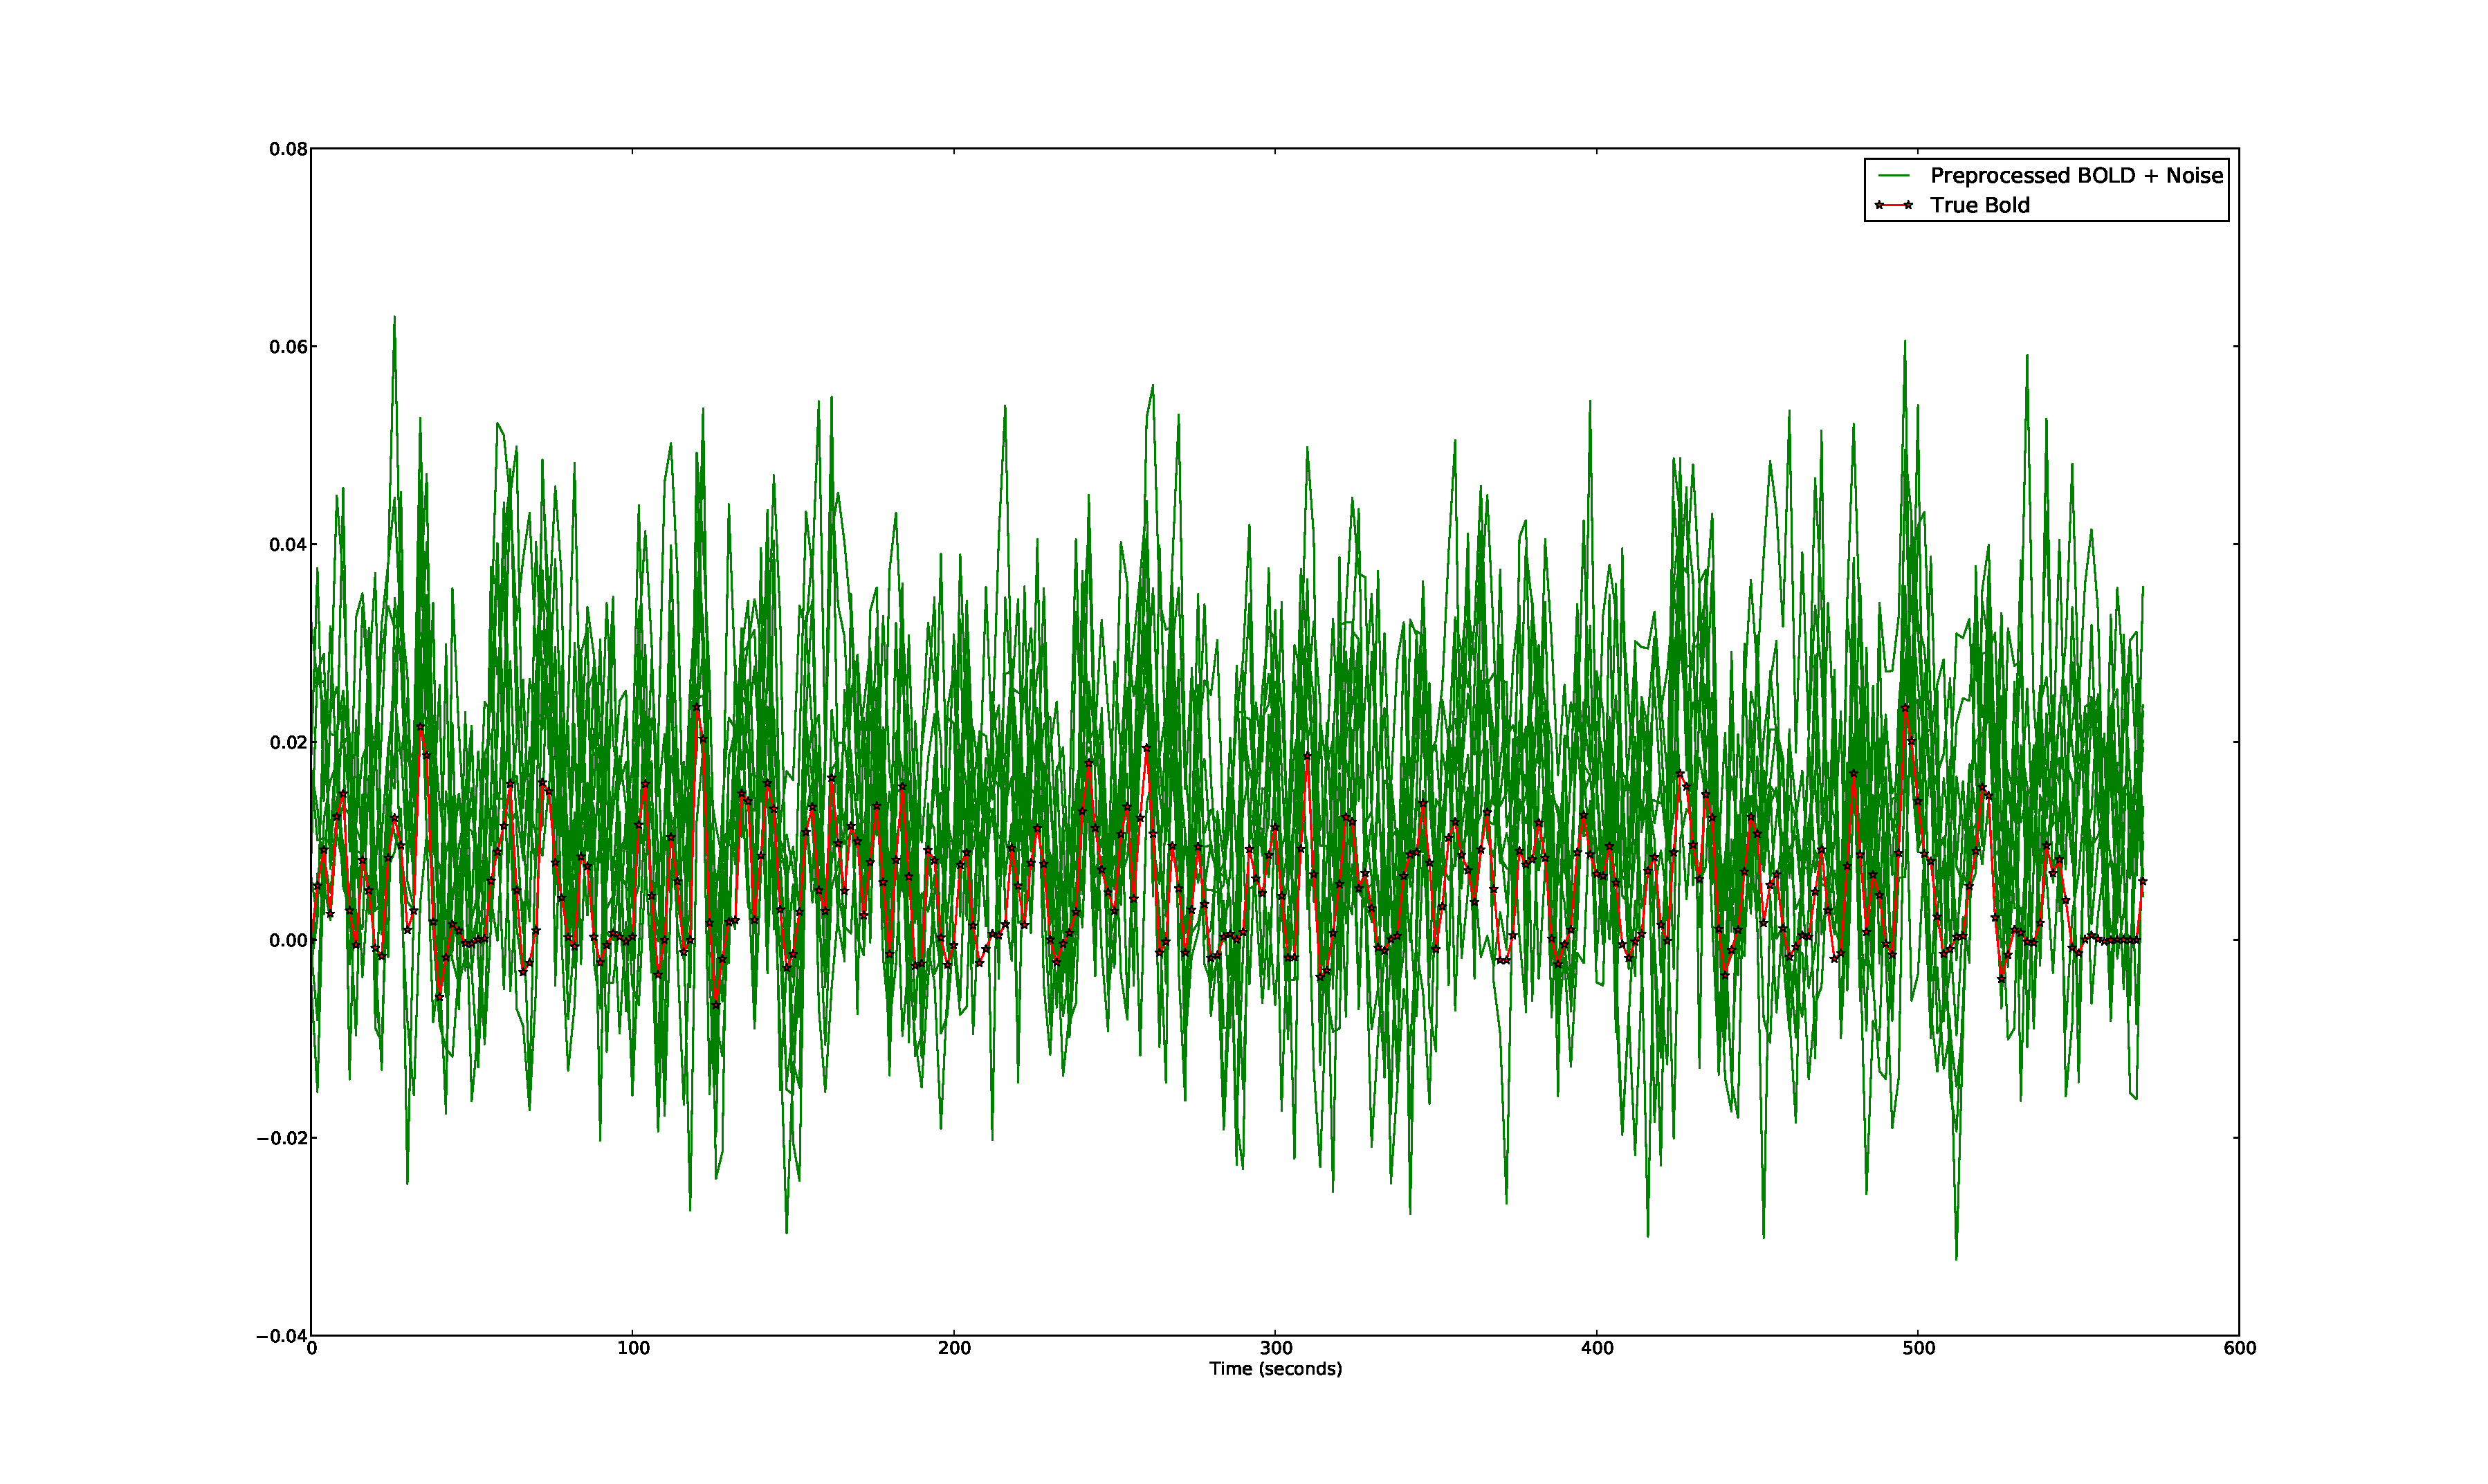
\includegraphics[clip=true,trim=6cm 2cm 6cm 3.5cm,width=17cm]{images/preprocessed_highnoise}
\caption{A comparison of the preprocessed signals for the high noise case.}
\label{fig:PreprocessedHighNoise}
\end{figure}
\begin{figure}
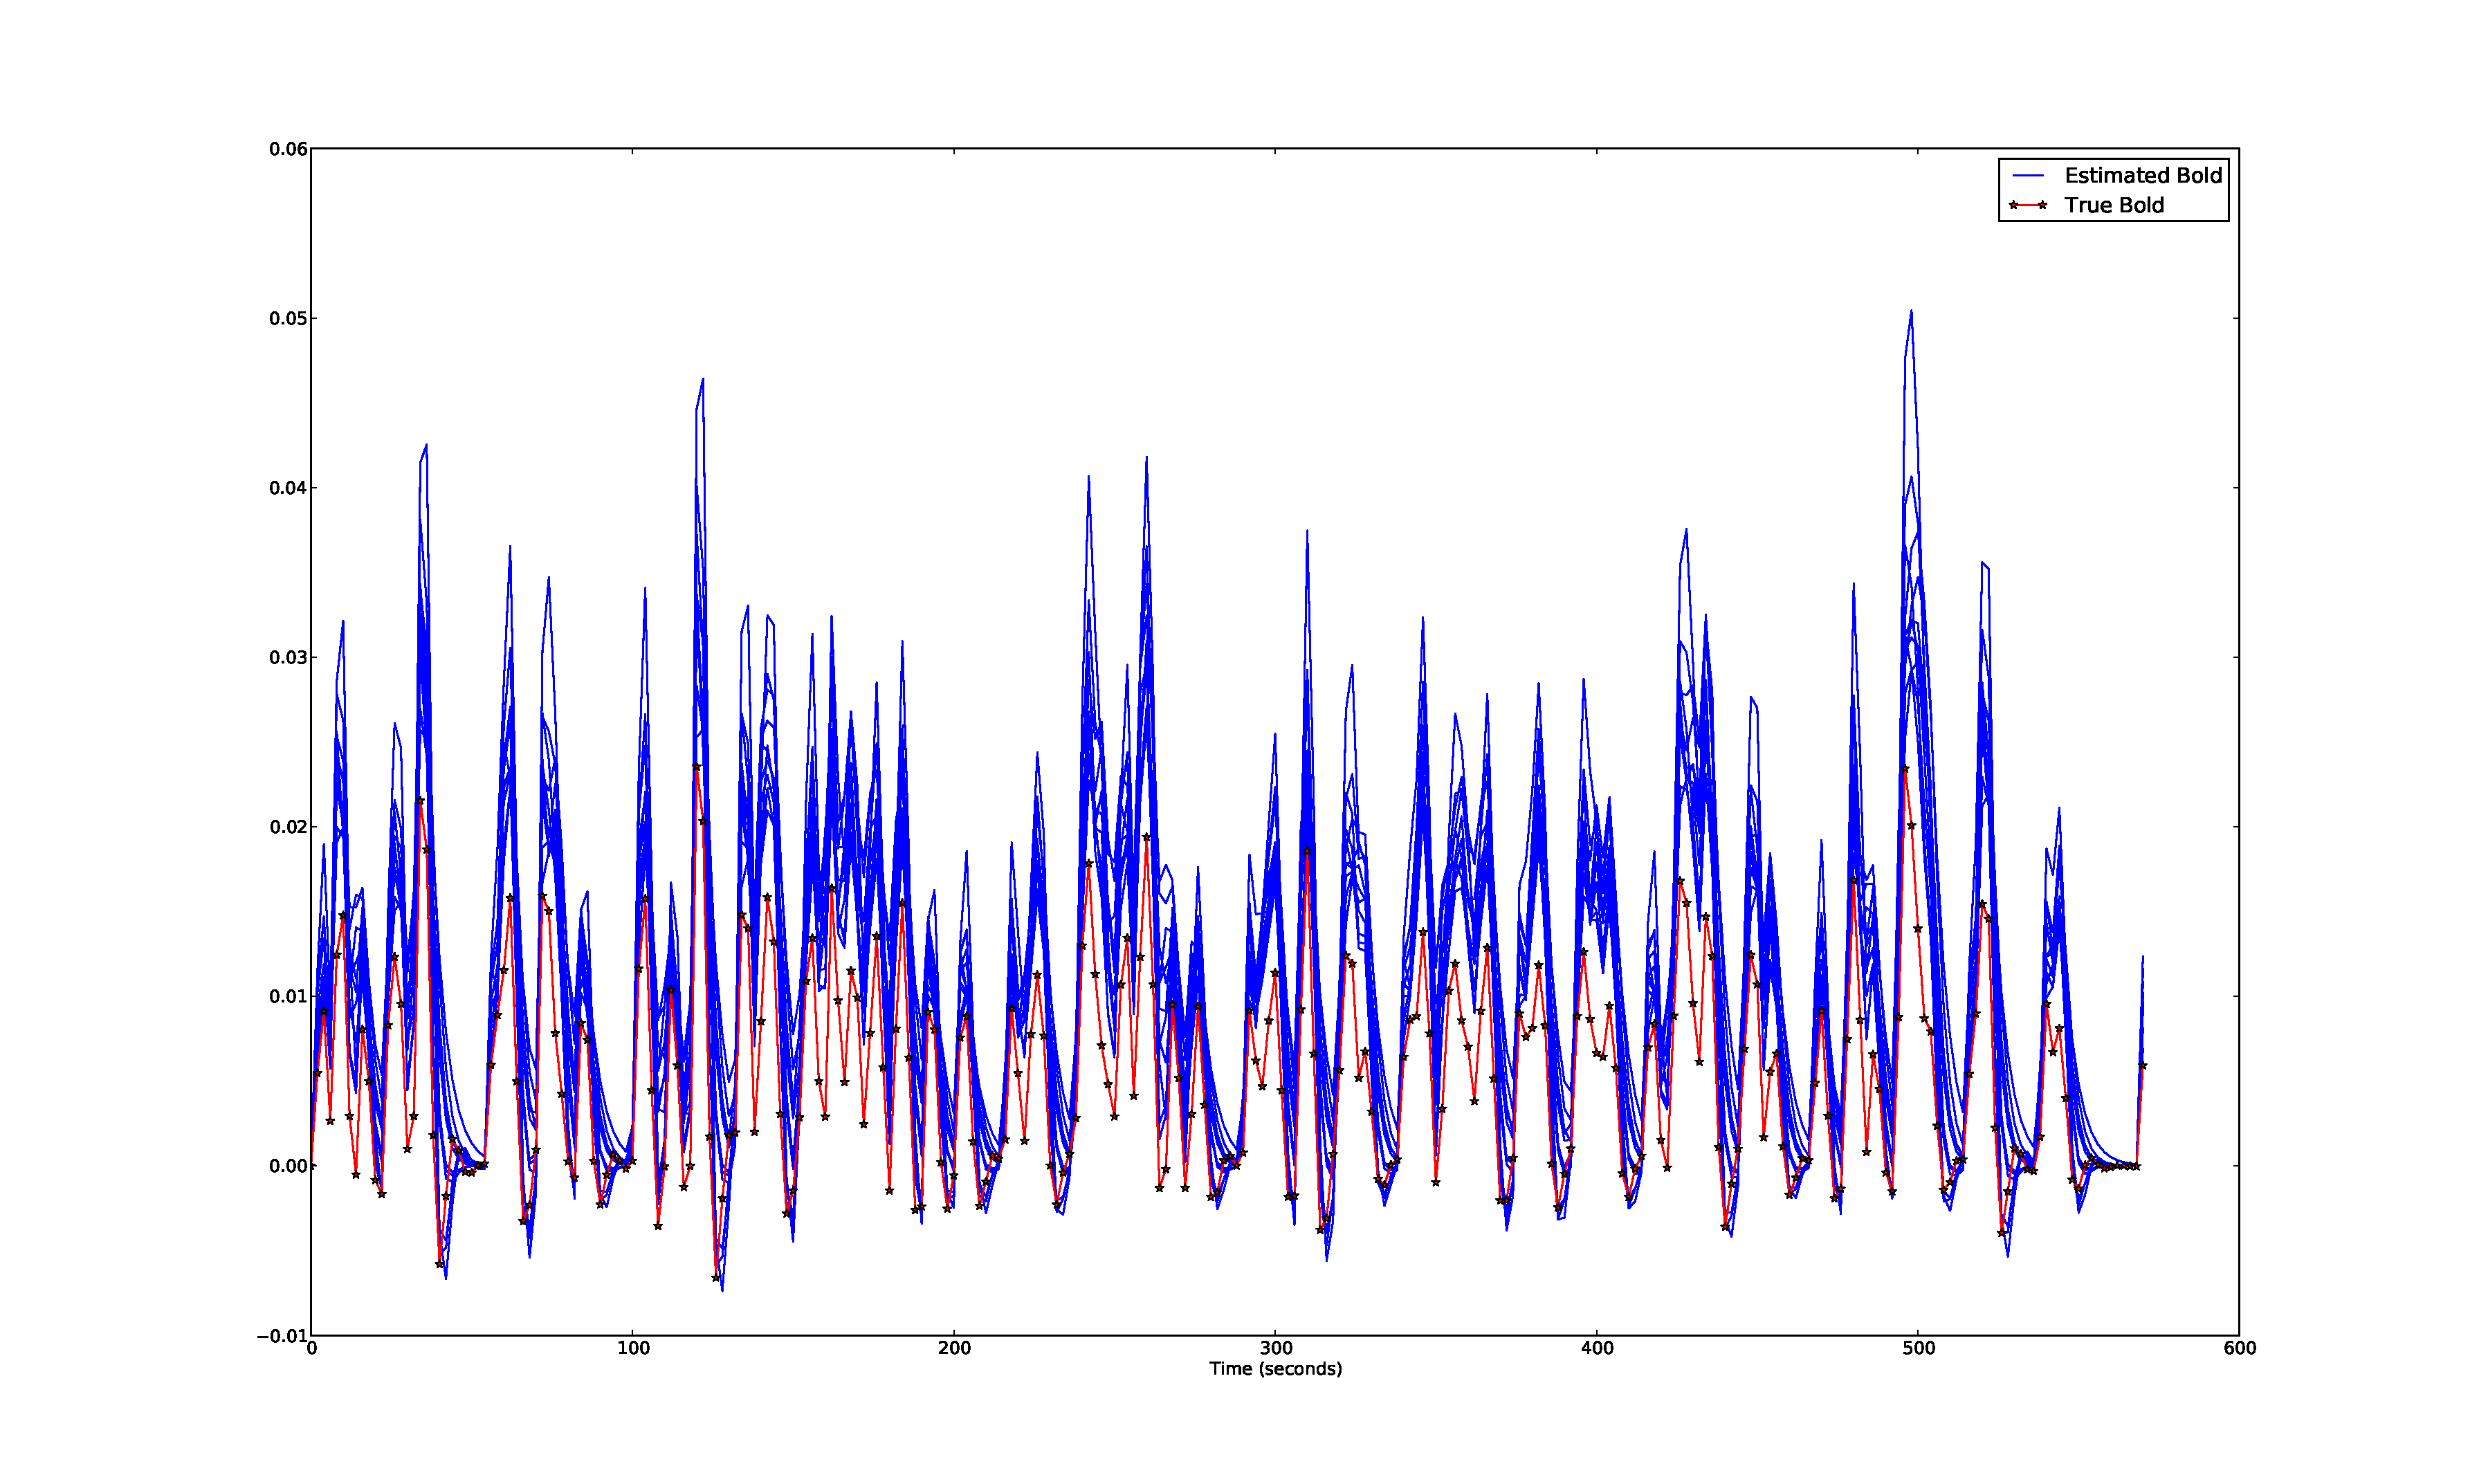
\includegraphics[clip=true,trim=6cm 2cm 6cm 3.5cm,width=17cm]{images/comparison_highnoise}
\caption{A comparison of the fitted signals for the high noise case.}
\label{fig:FitComparisonHighNoise}
\end{figure}
\begin{figure}
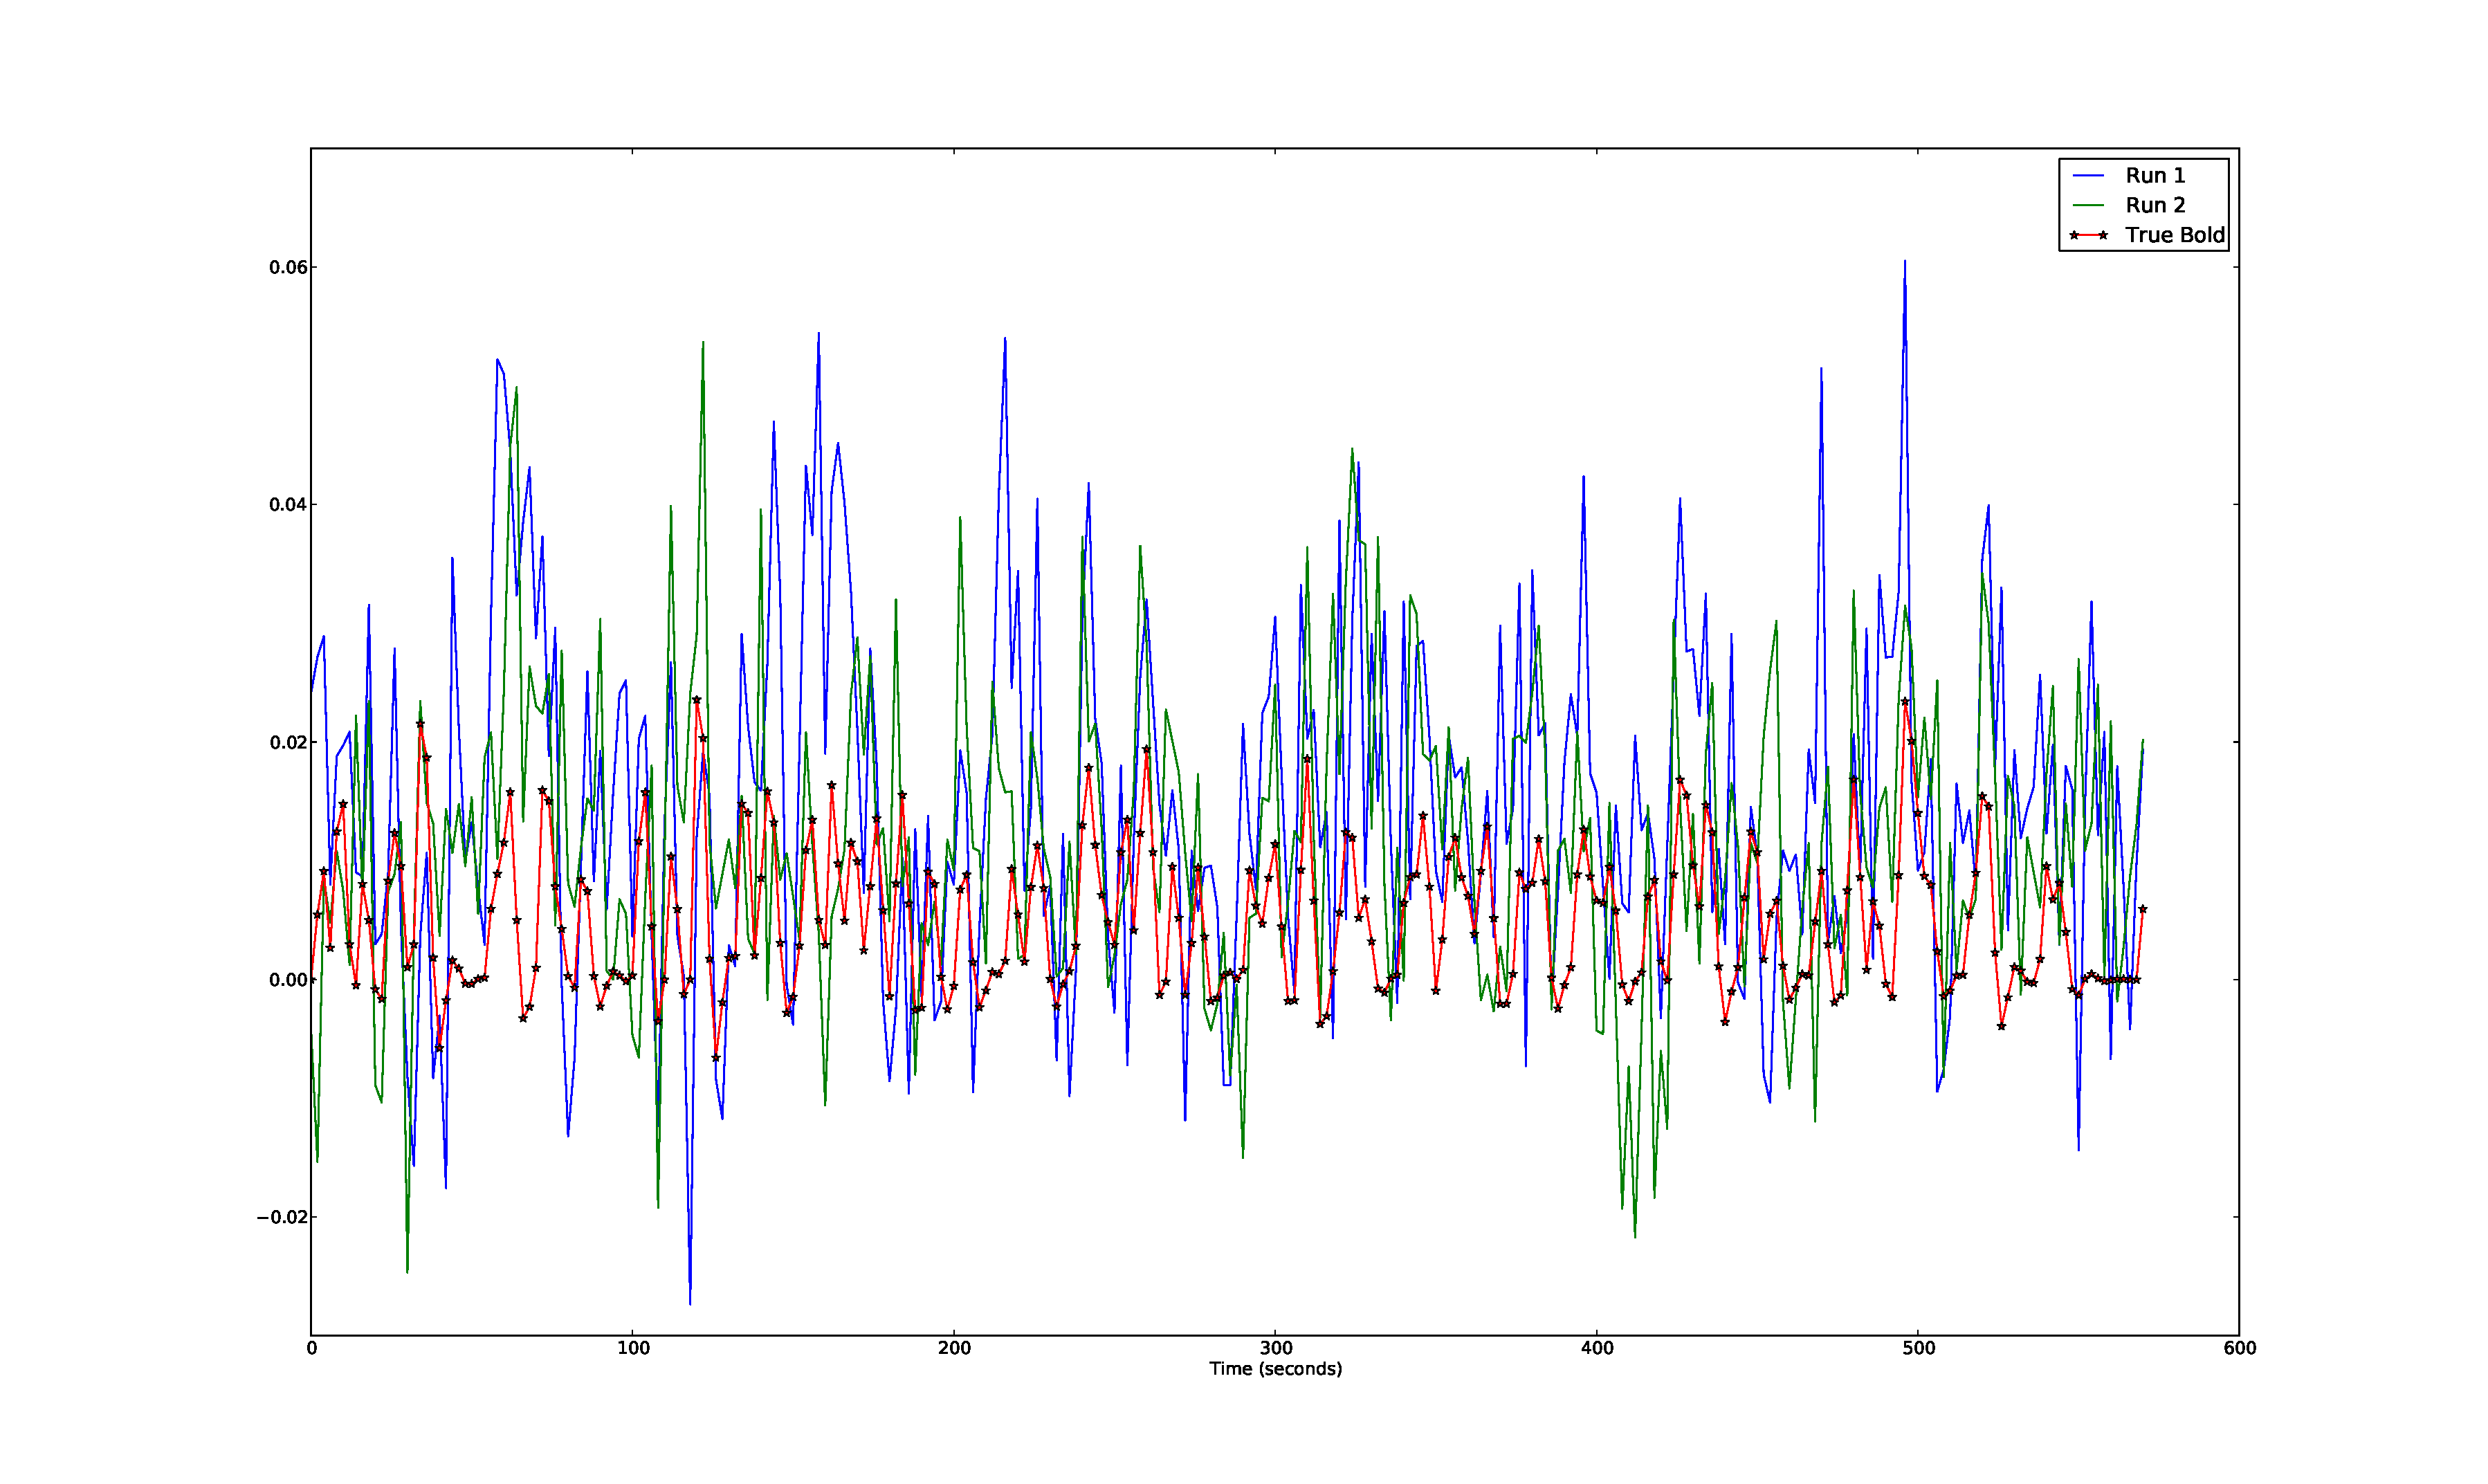
\includegraphics[clip=true,trim=6cm 2cm 6cm 3.5cm,width=17cm]{images/highnoise_56_noise}
\caption{Two particular preprocessed noise realizations for the high noise case.}
\label{fig:NoiseComparisonJustTwo}
\end{figure}

\begin{figure}
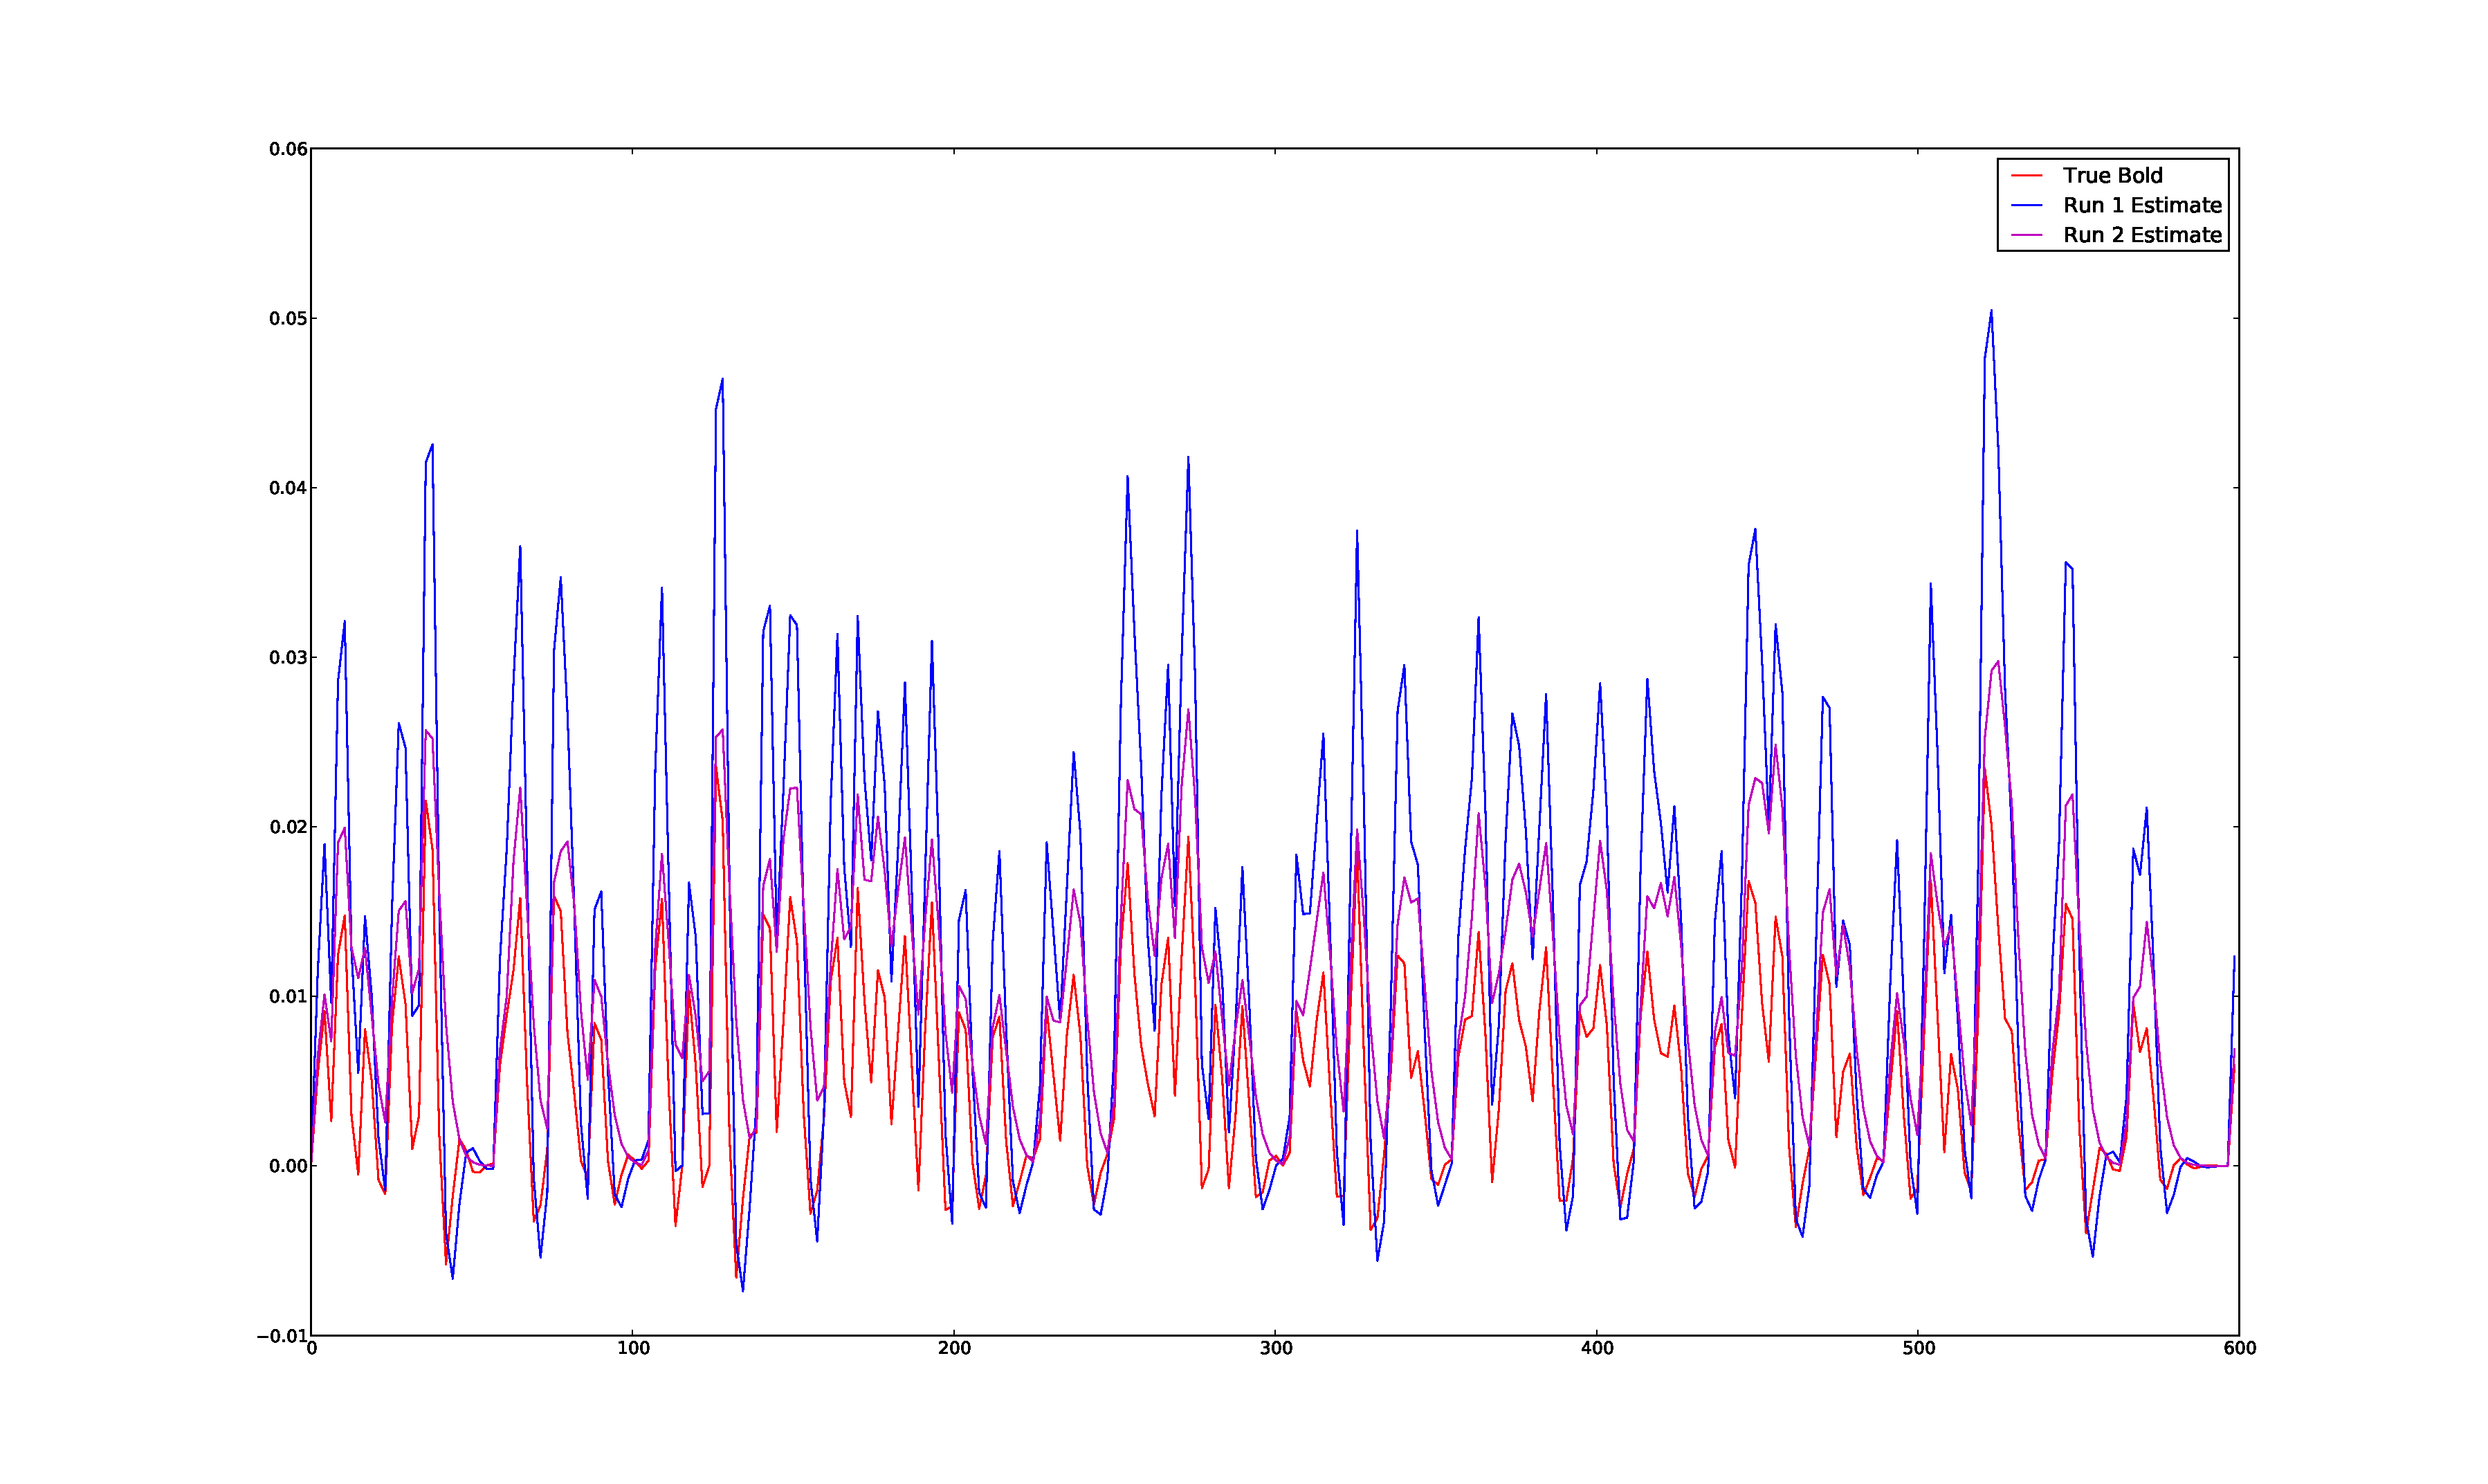
\includegraphics[clip=true,trim=6cm 2cm 6cm 3.5cm,width=17cm]{images/comparison_highnoise_just2}
\caption{The results for the noise realizations shown in \autoref{fig:NoiseComparisonJustTwo}.}
\label{fig:FitComparisonHighNoiseJust2}
\end{figure}

For the high noise simulation, the exact same procedure was performed as with the lower
noise simulation except that $\sigma_y$ and $\sigma_x$ were set to $.01$ and $.005$,
respectively. This an order of magnitude higher than the previous tests, and indeed the
noise appears to dominate the output, as seen in \autoref{fig:HighNoiseRealization}.  
As before, the results of preprocessing are helpful in identifying the reason for
bias in the estimated output signal; thus the preprocessed signals are shown in 
\autoref{fig:PreprocessedHighNoise}. The results of the particle filter
for each of the eleven runs are shown in \autoref{fig:FitComparisonHighNoise}. 
As before, the preprocessing led the algorithm
to somewhat higher activation levels, and it would appear that the subtleties of
different time constants are being lost due to the noise. This is easily seen
by observing the post stimulus undershoots; many of the estimated time series
have no post-stimulus undershoot but rather decay directly to the base level.

\begin{table}[t]
\centering
\begin{tabular}{|c | c | c | c | c | c | c | c | c | c |}
\hline 
$\tau_0$ & $\alpha$ & $E_0$    & $V_0$    & $\tau_s$ & $\tau_f$ & $\epsilon$  & $ \sum \tau $ & $\sqrt{MSR}$  & $\sqrt{MSE}$\\
\hline 
\rowcolor[gray]{.8}
1.45 & .3 & .47 & .044 & 1.94 & 1.99 & 1.8  & 5.38 &  & \\
\hline 
\hline 
1.1900 & 0.2349 & 0.4223 & 0.128  & 1.0147 & 2.4779 & 1.1168 & 4.6826 &0.01406 &0.01573   \\
0.9721 & 0.2190 & 0.3051 & 0.061  & 0.5780 & 1.9960 & 3.4613 & 3.5461 &0.01373 &0.01378   \\
1.5795 & 0.1415 & 0.3380 & 0.1089 & 0.5843 & 2.1247 & 1.7834 & 4.2885 &0.01275 &0.01577   \\
1.1094 & 0.2374 & 0.5349 & 0.0351 & 1.2186 & 3.0736 & 2.3504 & 5.4016 &0.01673 &0.01154    \\
1.1071 & 0.2753 & 0.3365 & 0.0316 & 1.5057 & 2.6518 & 4.1910 & 5.2646 &0.01370 &0.01222   \\
0.5803 & 0.4793 & 0.4135 & 0.1189 & 0.9756 & 3.6902 & 1.0008 & 5.2461 &0.01150 &0.01316   \\
\rowcolor[rgb]{.9,.5,.5}
1.2952 & 0.2596 & 0.2756 & 0.2595 & 1.7026 & 2.8458 & 0.6617 & 5.8436 &0.01555 &0.01790   \\
\rowcolor[rgb]{.5,.5,.9}
1.5185 & 0.2199 & 0.2835 & 0.0742 & 0.8882 & 3.0771 & 1.7393 & 5.4838 &0.01205 &0.01246   \\
0.6874 & 0.3283 & 0.3979 & 0.1561 & 1.0778 & 3.1158 & 0.6643 & 4.8810 &0.01510 &0.01258   \\
1.0170 & 0.285  & 0.3474 & 0.0567 & 1.5877 & 2.6516 & 2.2852 & 5.2563 &0.01249 &0.01343   \\
0.9925 & 0.298  & 0.3221 & 0.2094 & 0.4276 & 2.2108 & 1.0167 & 3.6308 &0.01217 &0.01506   \\
\hline                                                                          
1.0954 & 0.2708 & 0.3615 & 0.1126 & 1.0510 & 2.7196 & 1.8428 & 4.8659 &0.01362 &0.01397\\
\hline 
\end{tabular}
\caption{Estimated Parameters on 10 different runs with high noise. First row is the true parameters.
Note also that the red row is Run 1 and the blue row is Run 2, as named in  \autoref{fig:NoiseComparisonJustTwo}
and \autoref{fig:FitComparisonHighNoiseJust2}}
\label{tab:HighNoiseResults} 
\end{table}

It is interesting to consider how the preprocessing and noise may effect the
parameters of the fitting model. Consider two runs, shown in 
\autoref{fig:NoiseComparisonJustTwo}, out of the previous eleven. 
Run 1 clearly has higher peaks, in spite of the fact that both signals are based
on the same underlying signal. There also appears
to be more drift than the 20 measurements per knot could fit, which explains run 1's
prolonged increase at 170 seconds in. Interestingly, run 1 and run 2 have different
aspects of the signal that match better. Run 2 had a much better match to the 
peaks, when compared to the true signal, yet run 1 matched the post-stimulus
undershoot better. Its worth noting however, that the post-stimulus undershoots
here are much shorted than the observed prolonged post-stimulus undershoot
discussed in \autoref{sec:Post Stimulus Undershoot}. 
Despite the rather significant amount of noise, the ultimate results are 
actually rather good. \autoref{tab:HighNoiseResults} shows
the square-root mean-squared-error for all eleven runs, and highlights the two runs analyzed 
in \autoref{fig:ConvergenceRuns1} and \autoref{fig:ConvergenceRuns2}.

\begin{figure}
\subfigure[$\tau_0$, $\alpha$, $E_0$, $V_0$, Run 1]
{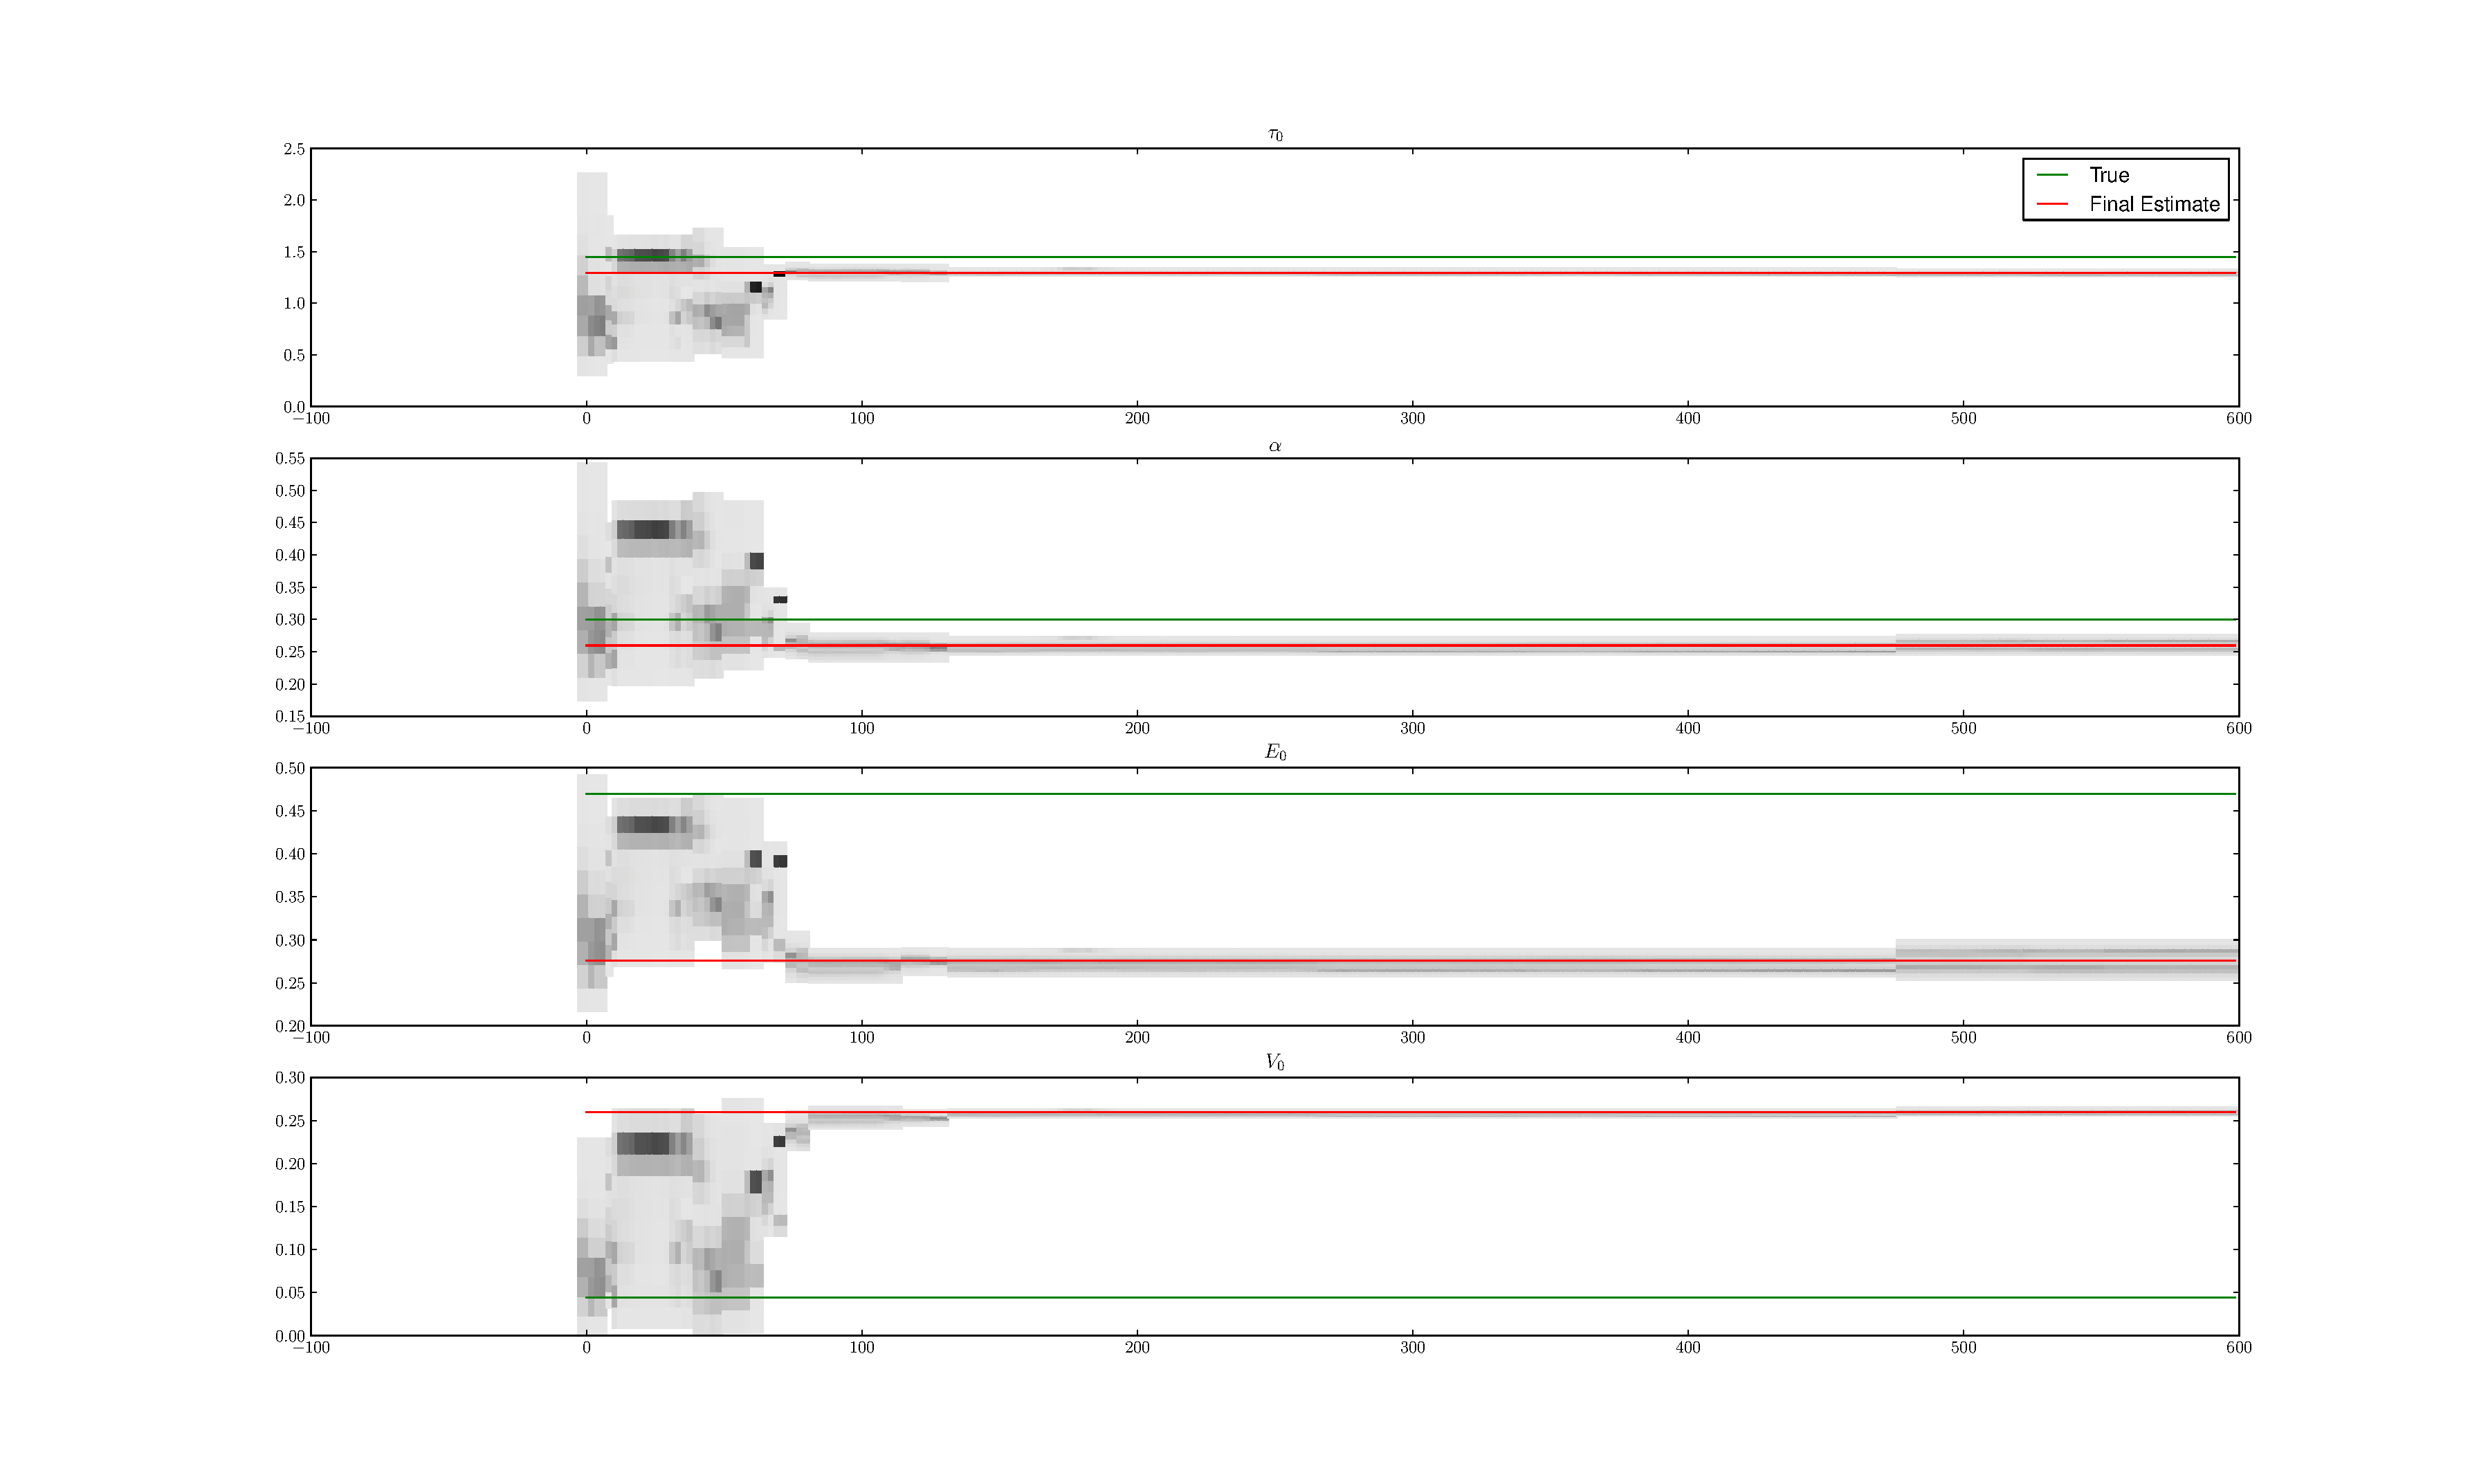
\includegraphics[clip=true,trim=6cm 2cm 6cm 3cm, width=14cm]{images/highnoise_run5_1}}\\
\end{figure}
\begin{figure}
\subfigure[$\tau_s$, $\tau_f$, $\epsilon$, $V$, Run 1] 
{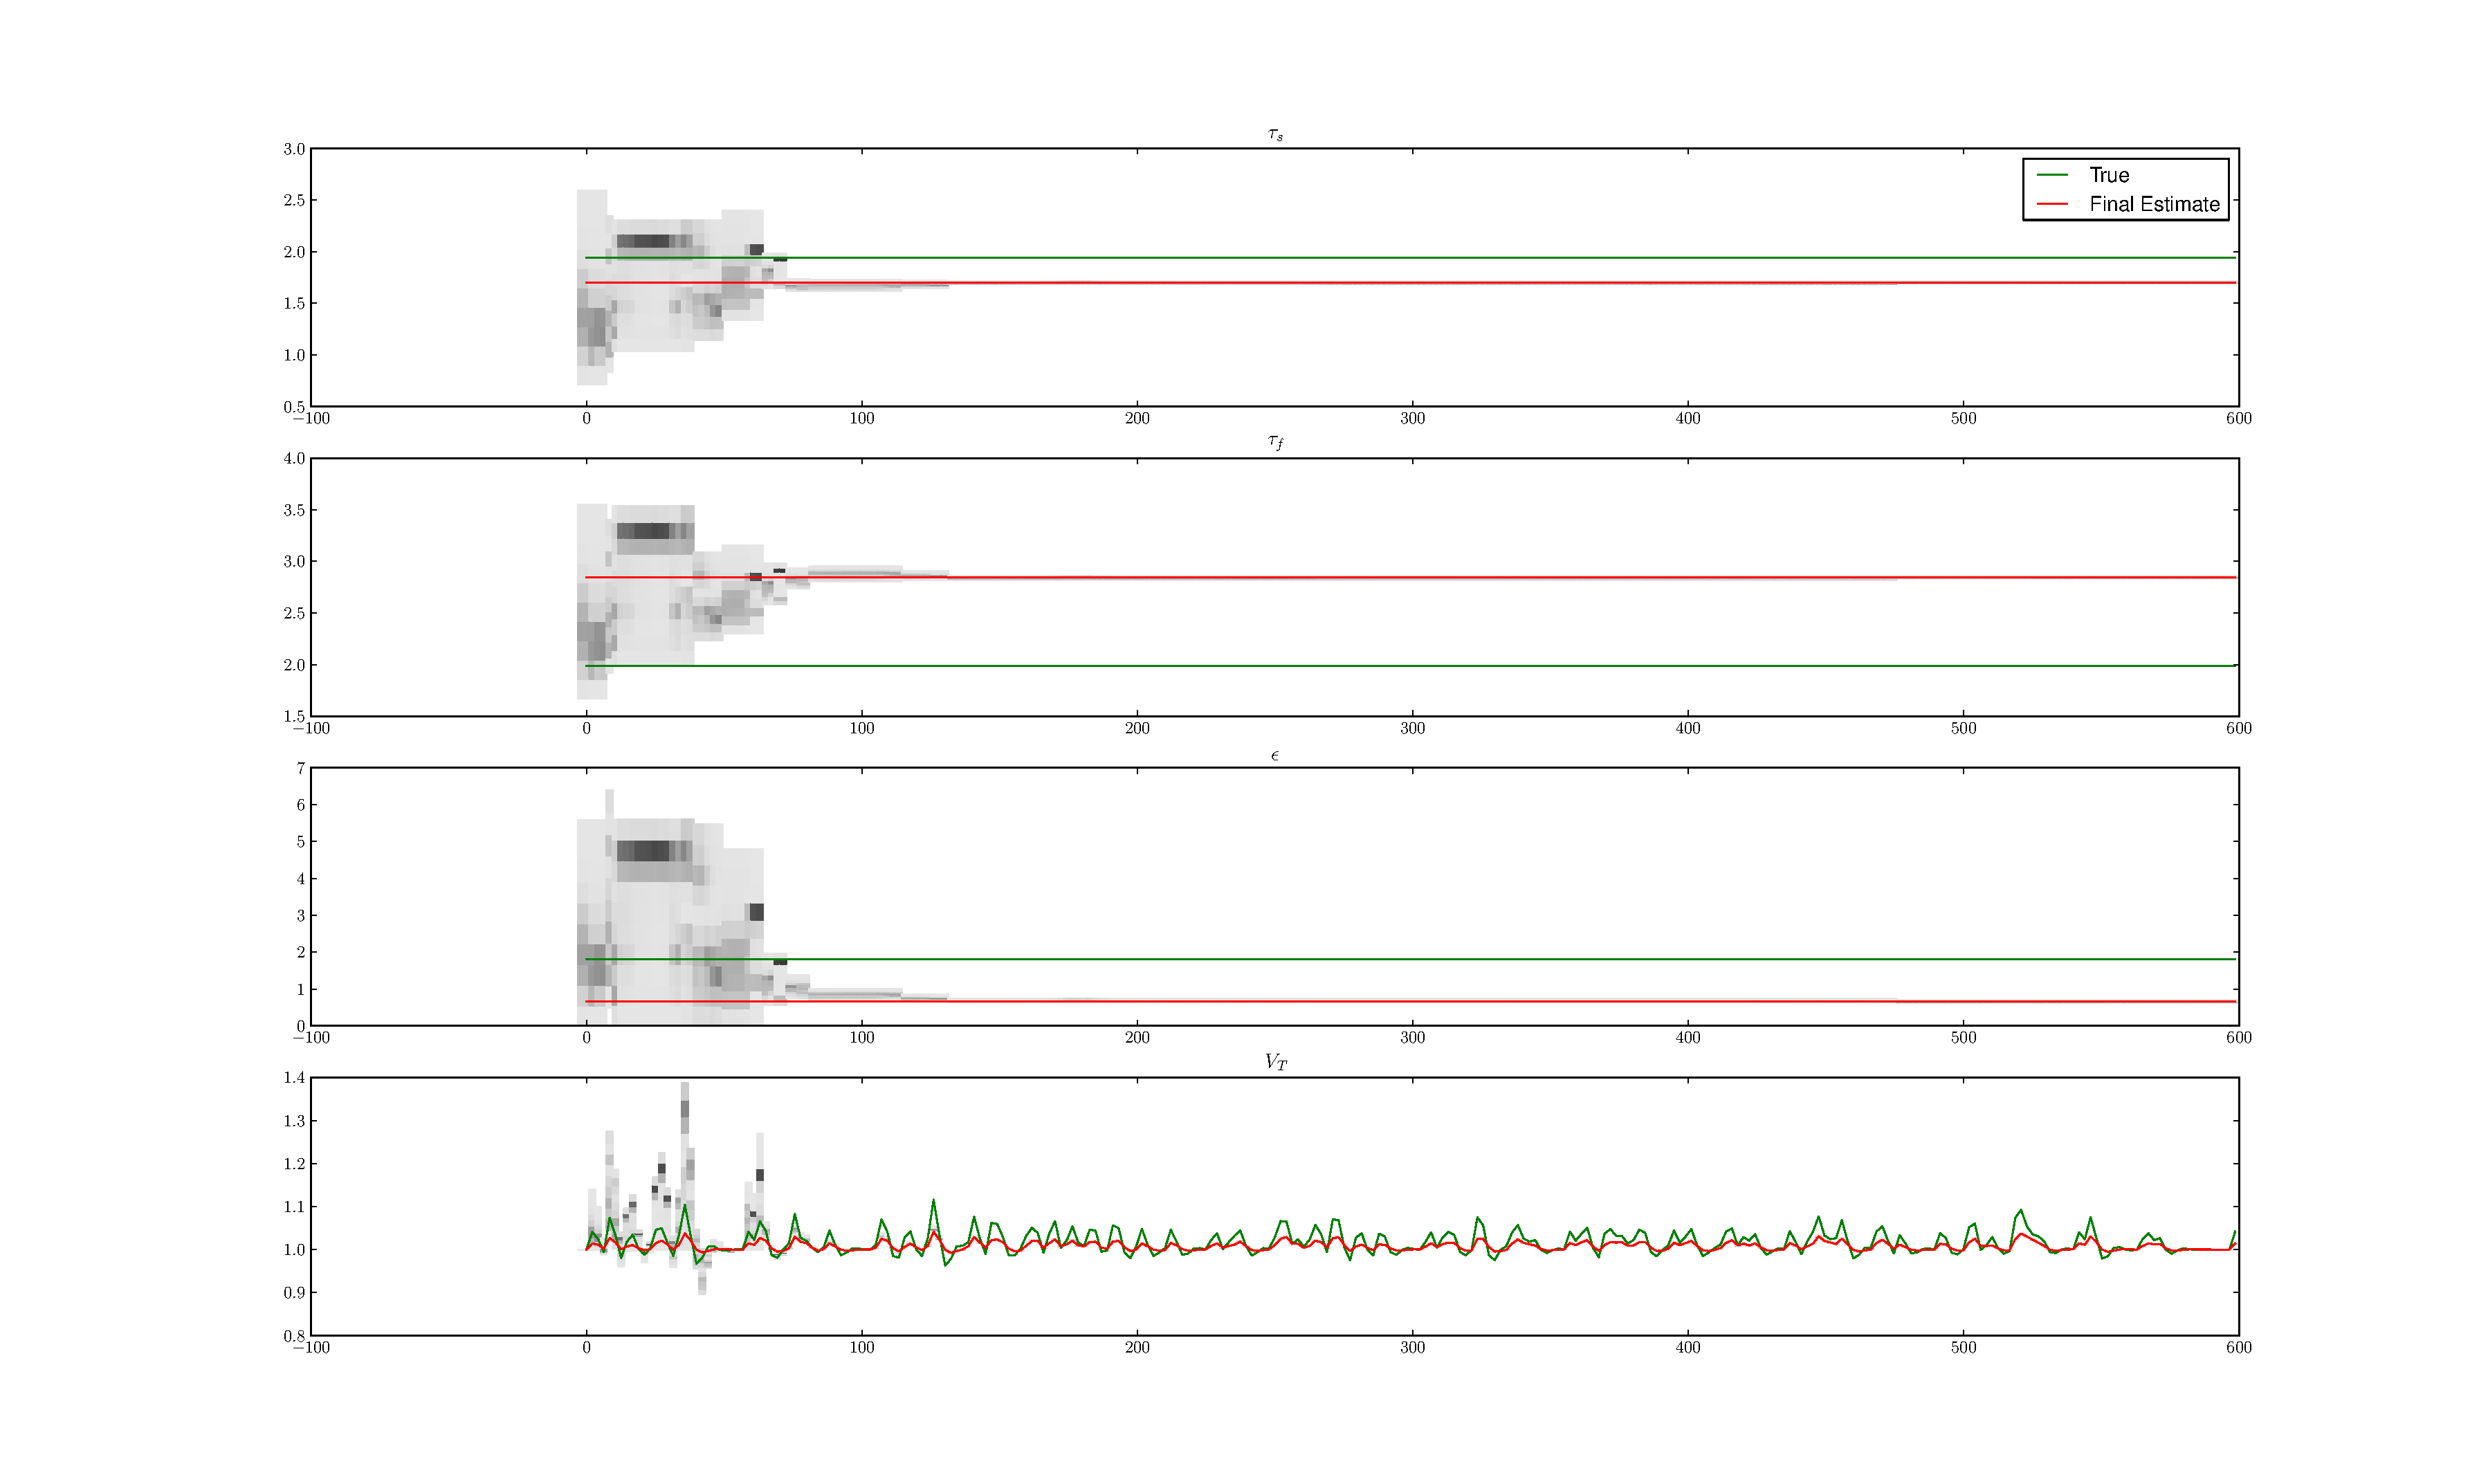
\includegraphics[clip=true,trim=6cm 2cm 6cm 3cm, width=14cm]{images/highnoise_run5_2}}\\
\end{figure}
\begin{figure}
\subfigure[$Q$, $S$, $F$, $BOLD$, Run 1 ]
{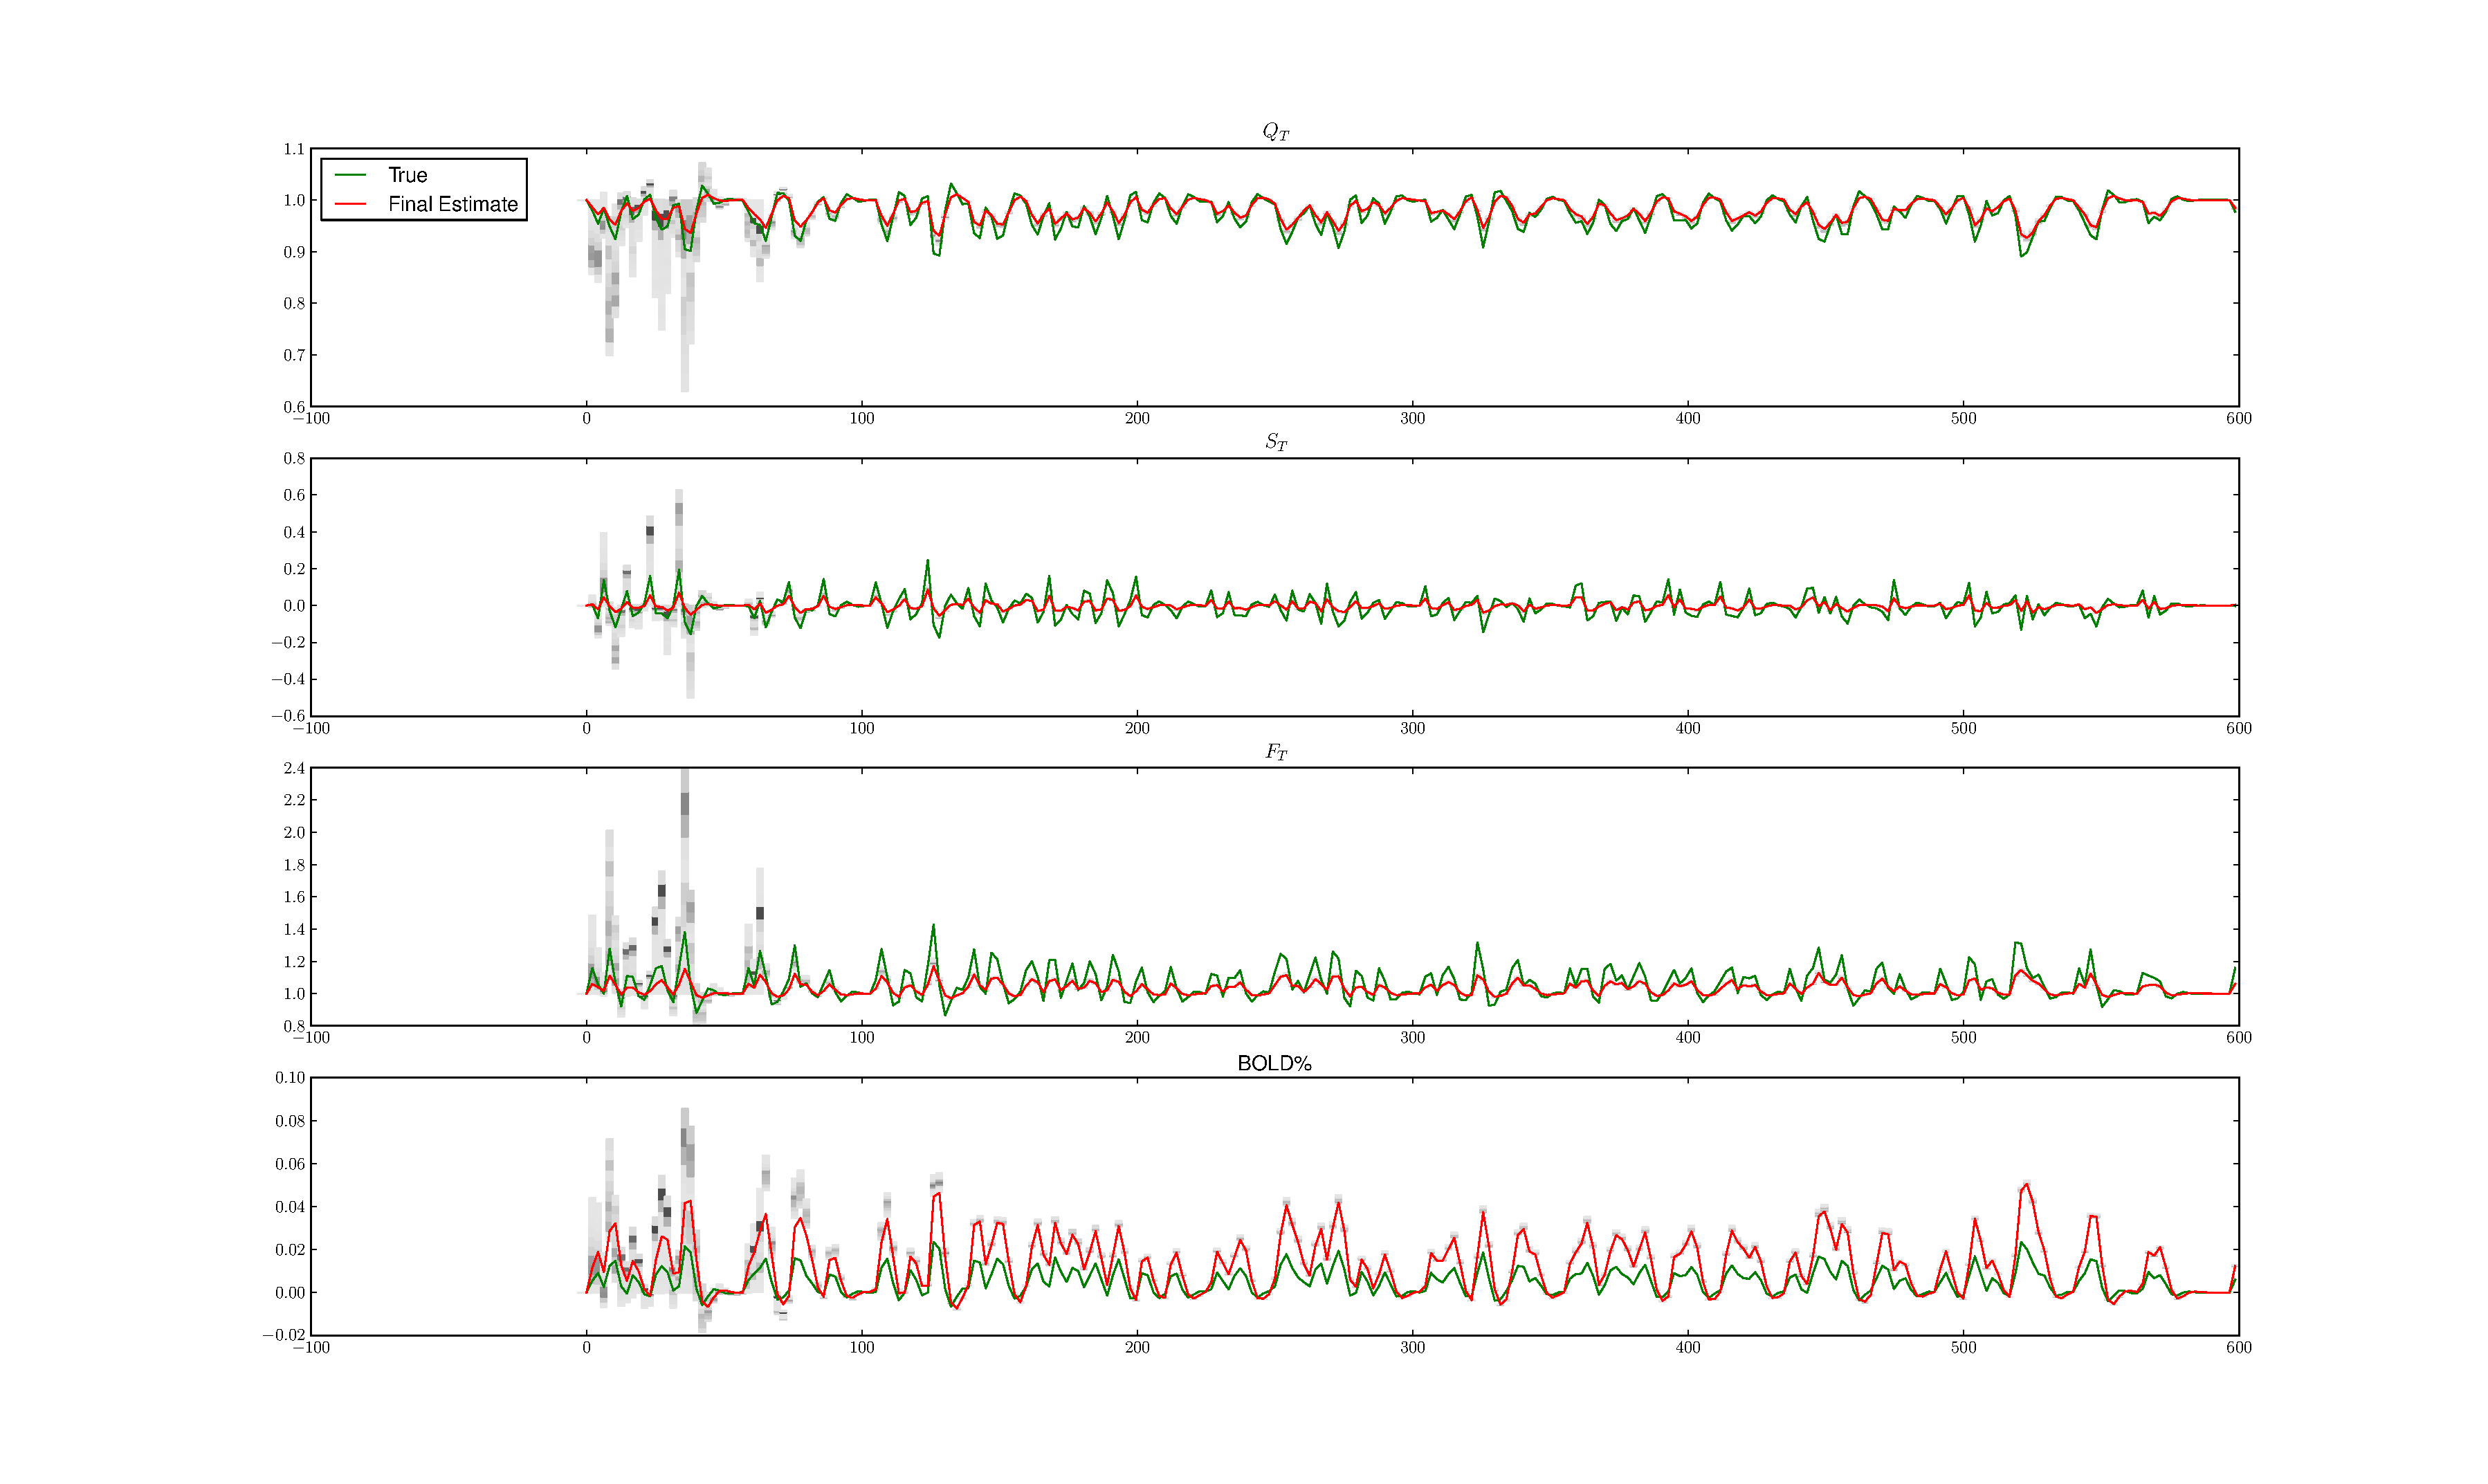
\includegraphics[clip=true,trim=6cm 2cm 6cm 3cm, width=14cm]{images/highnoise_run5_3}}
\caption{Converging histogram for parameters during run 1, as in \autoref{fig:NoiseComparisonJustTwo}.}
\label{fig:ConvergenceRuns1}
\end{figure}

\begin{figure}
\subfigure[$\tau_0$, $\alpha$, $E_0$, $V_0$, Run 2]
{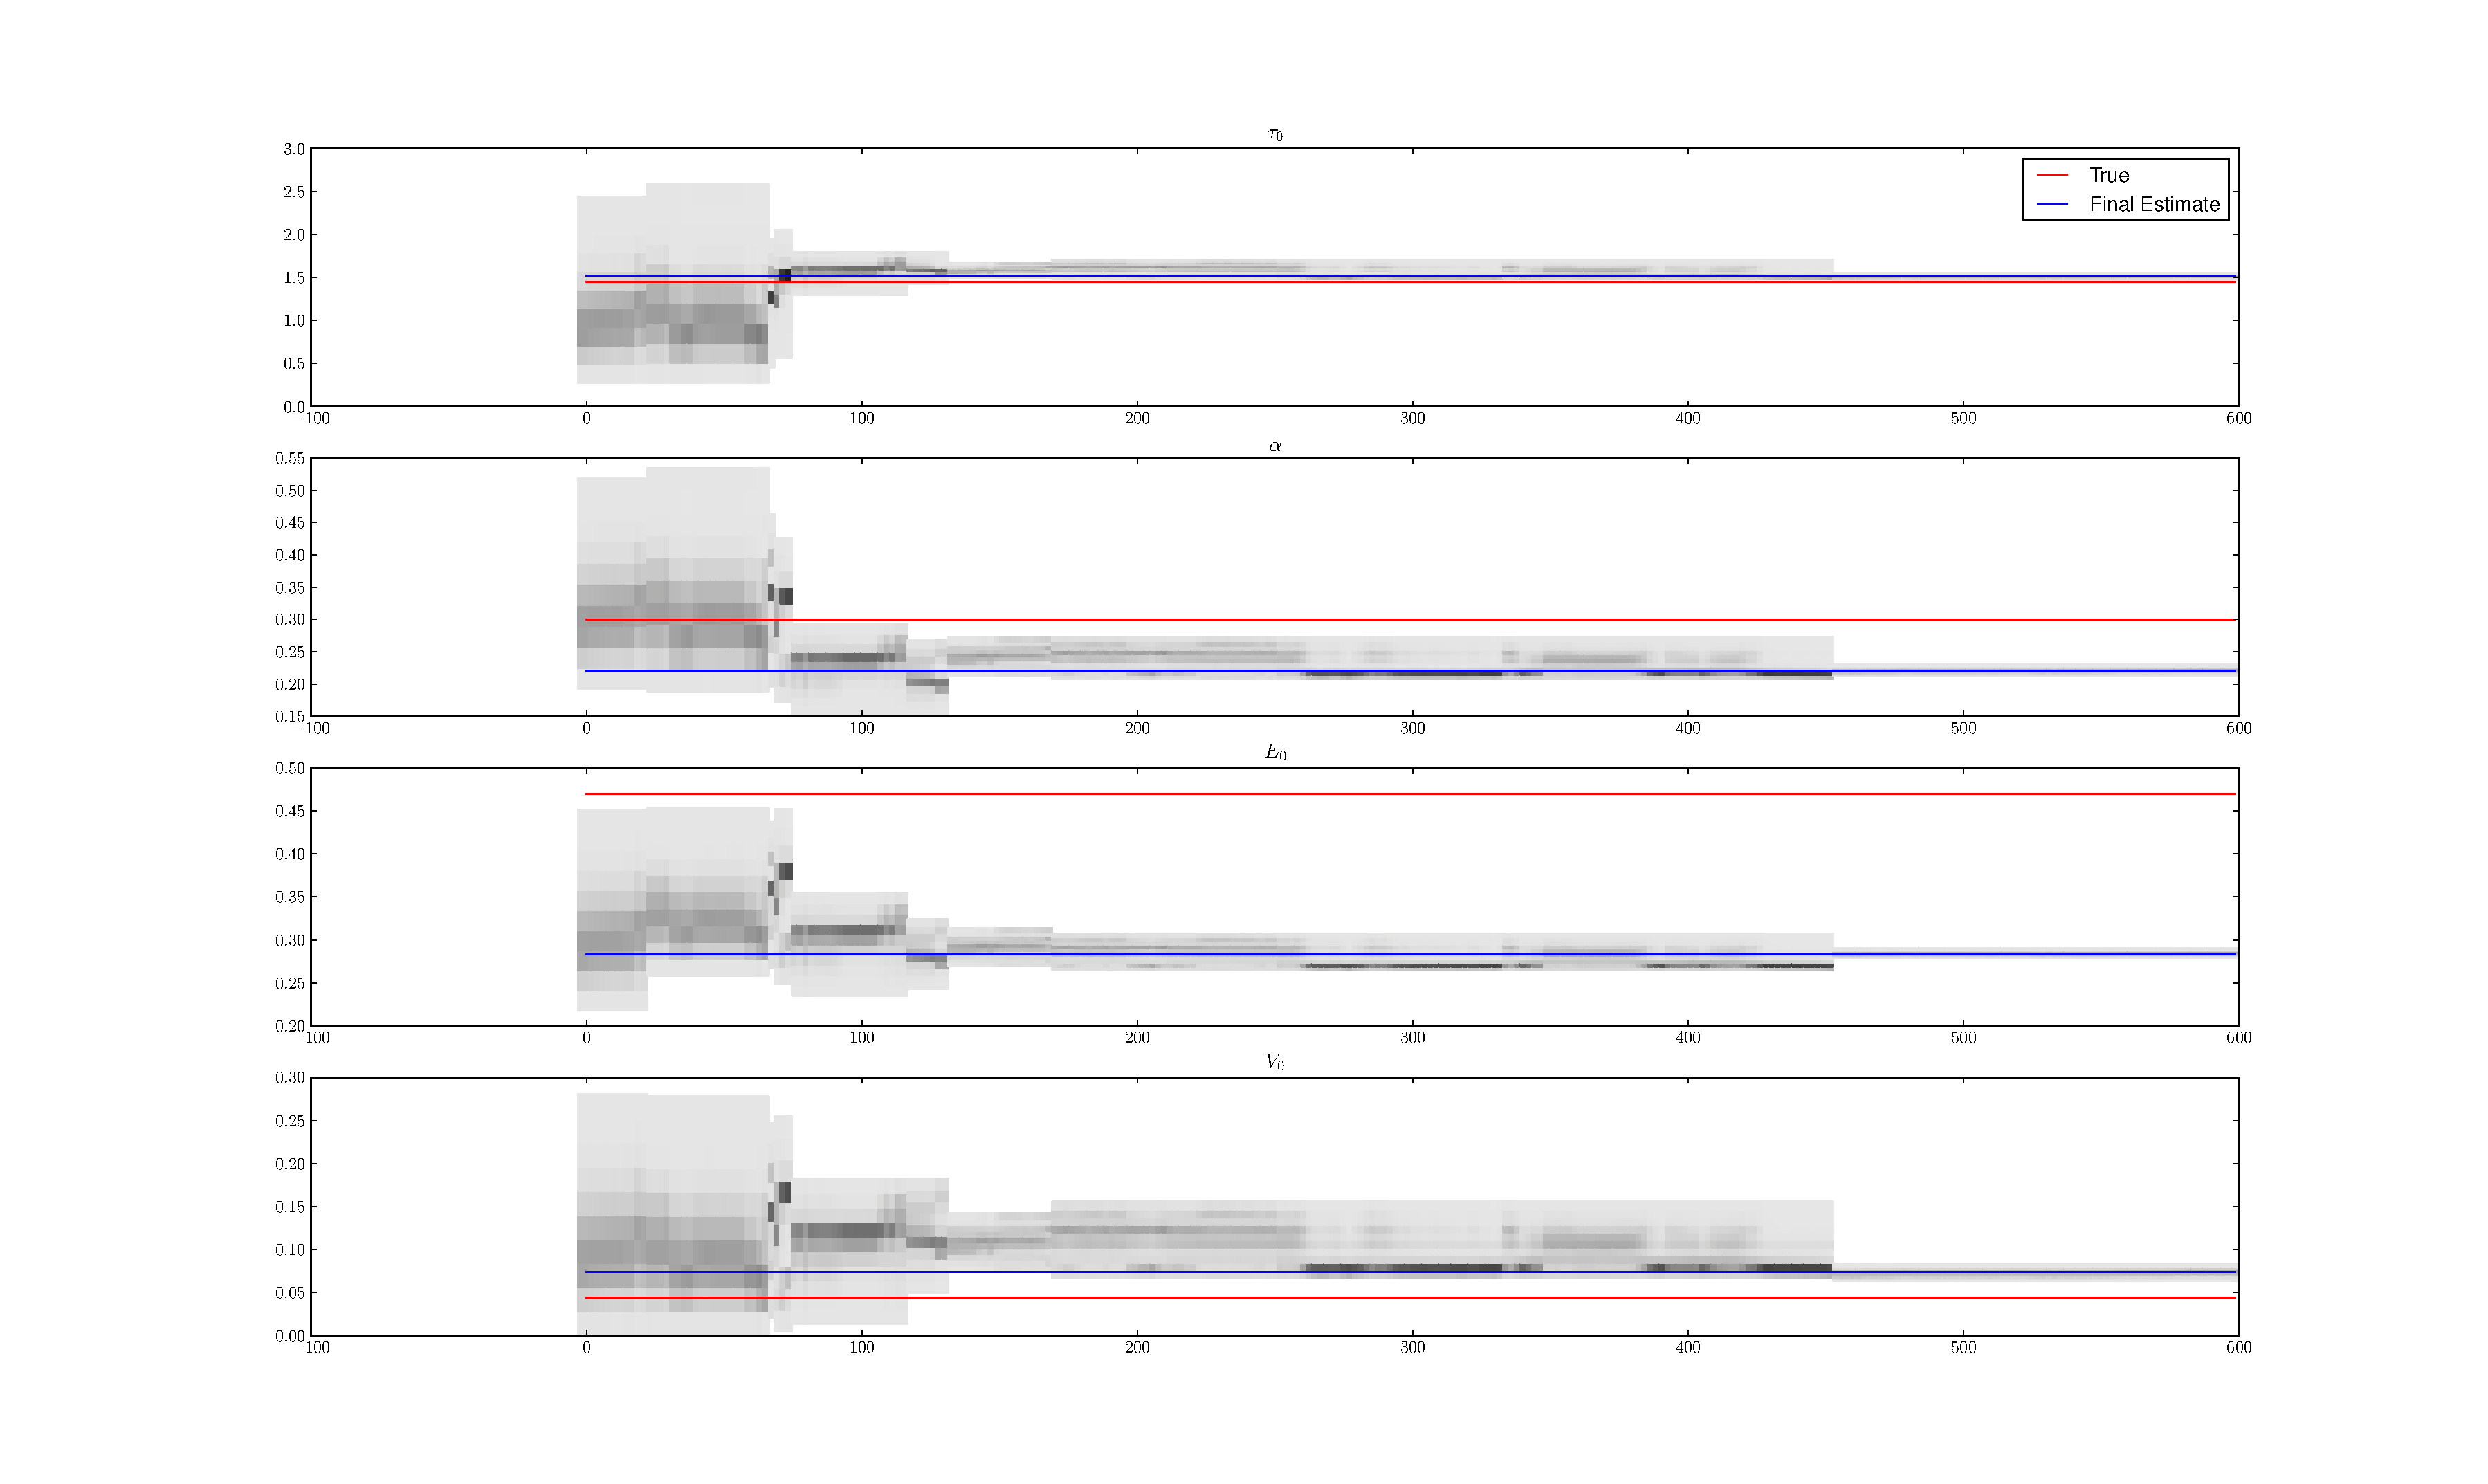
\includegraphics[clip=true,trim=6cm 2cm 6cm 3cm, width=14cm]{images/highnoise_run6_1}}\\
\end{figure}
\begin{figure}
\subfigure[$\tau_s$, $\tau_f$, $\epsilon$, $V$, Run 2] 
{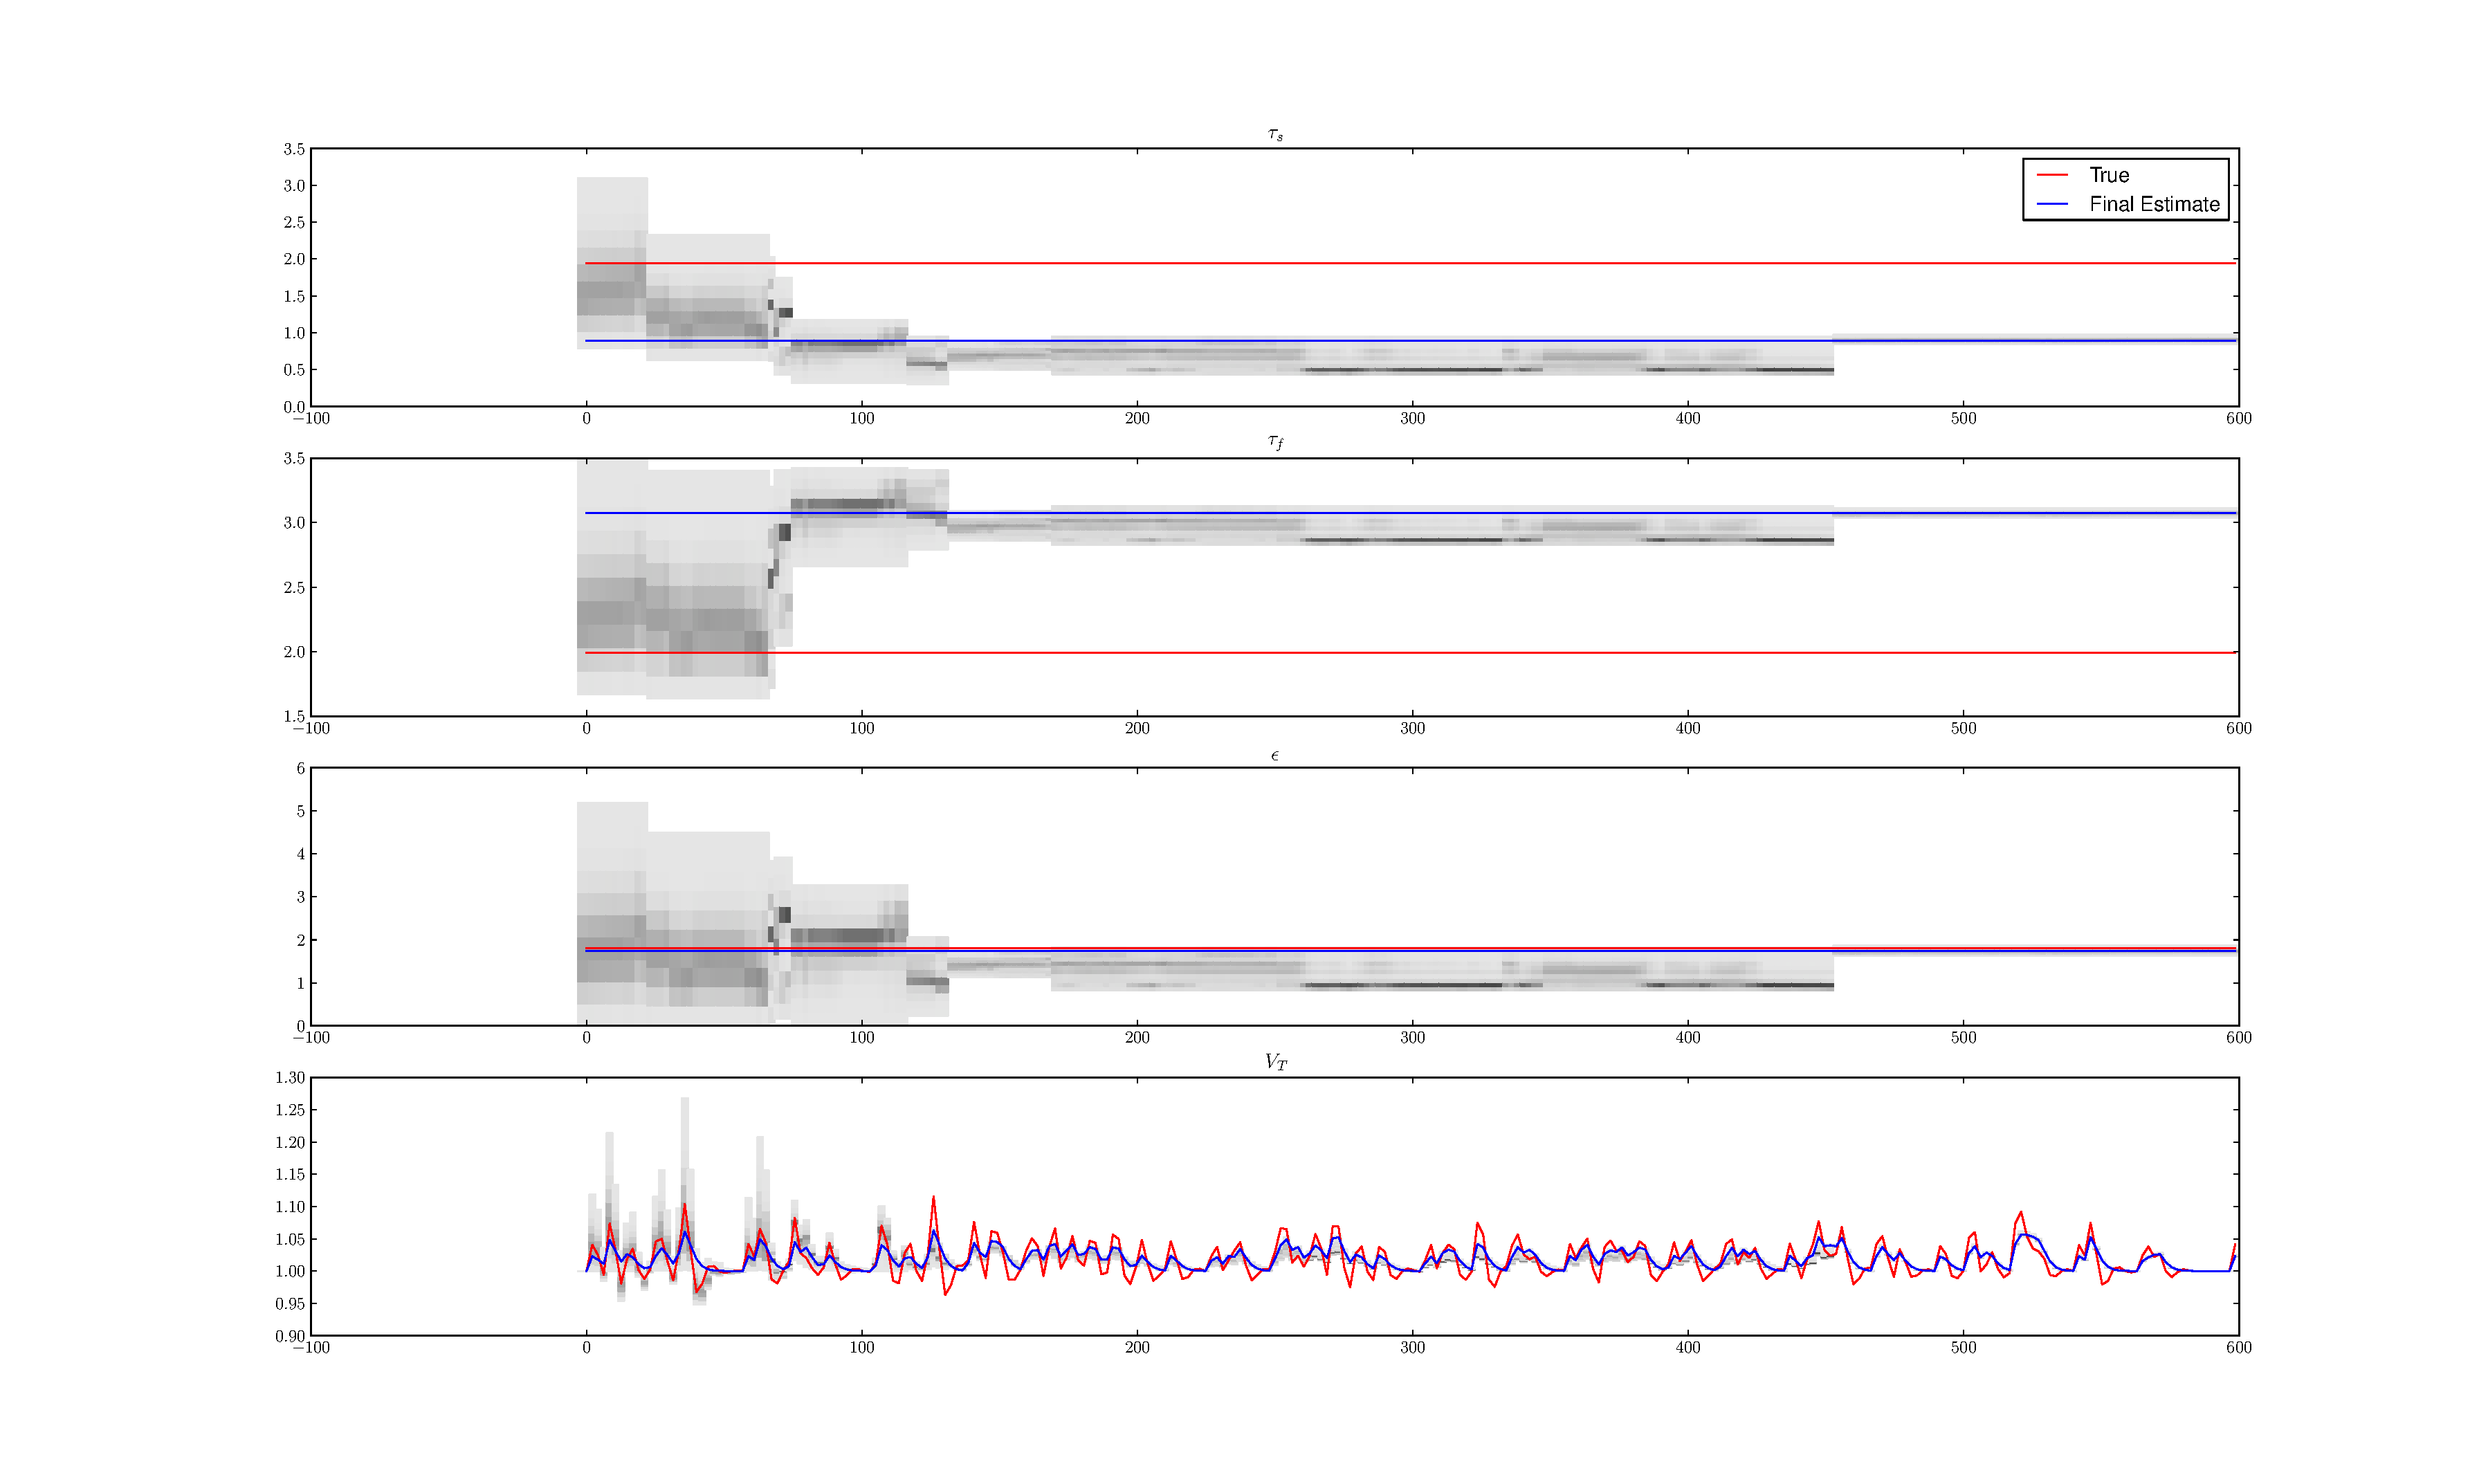
\includegraphics[clip=true,trim=6cm 2cm 6cm 3cm, width=14cm]{images/highnoise_run6_2}}\\
\end{figure}
\begin{figure}
\subfigure[$Q$, $S$, $F$, $BOLD$, Run 2 ]
{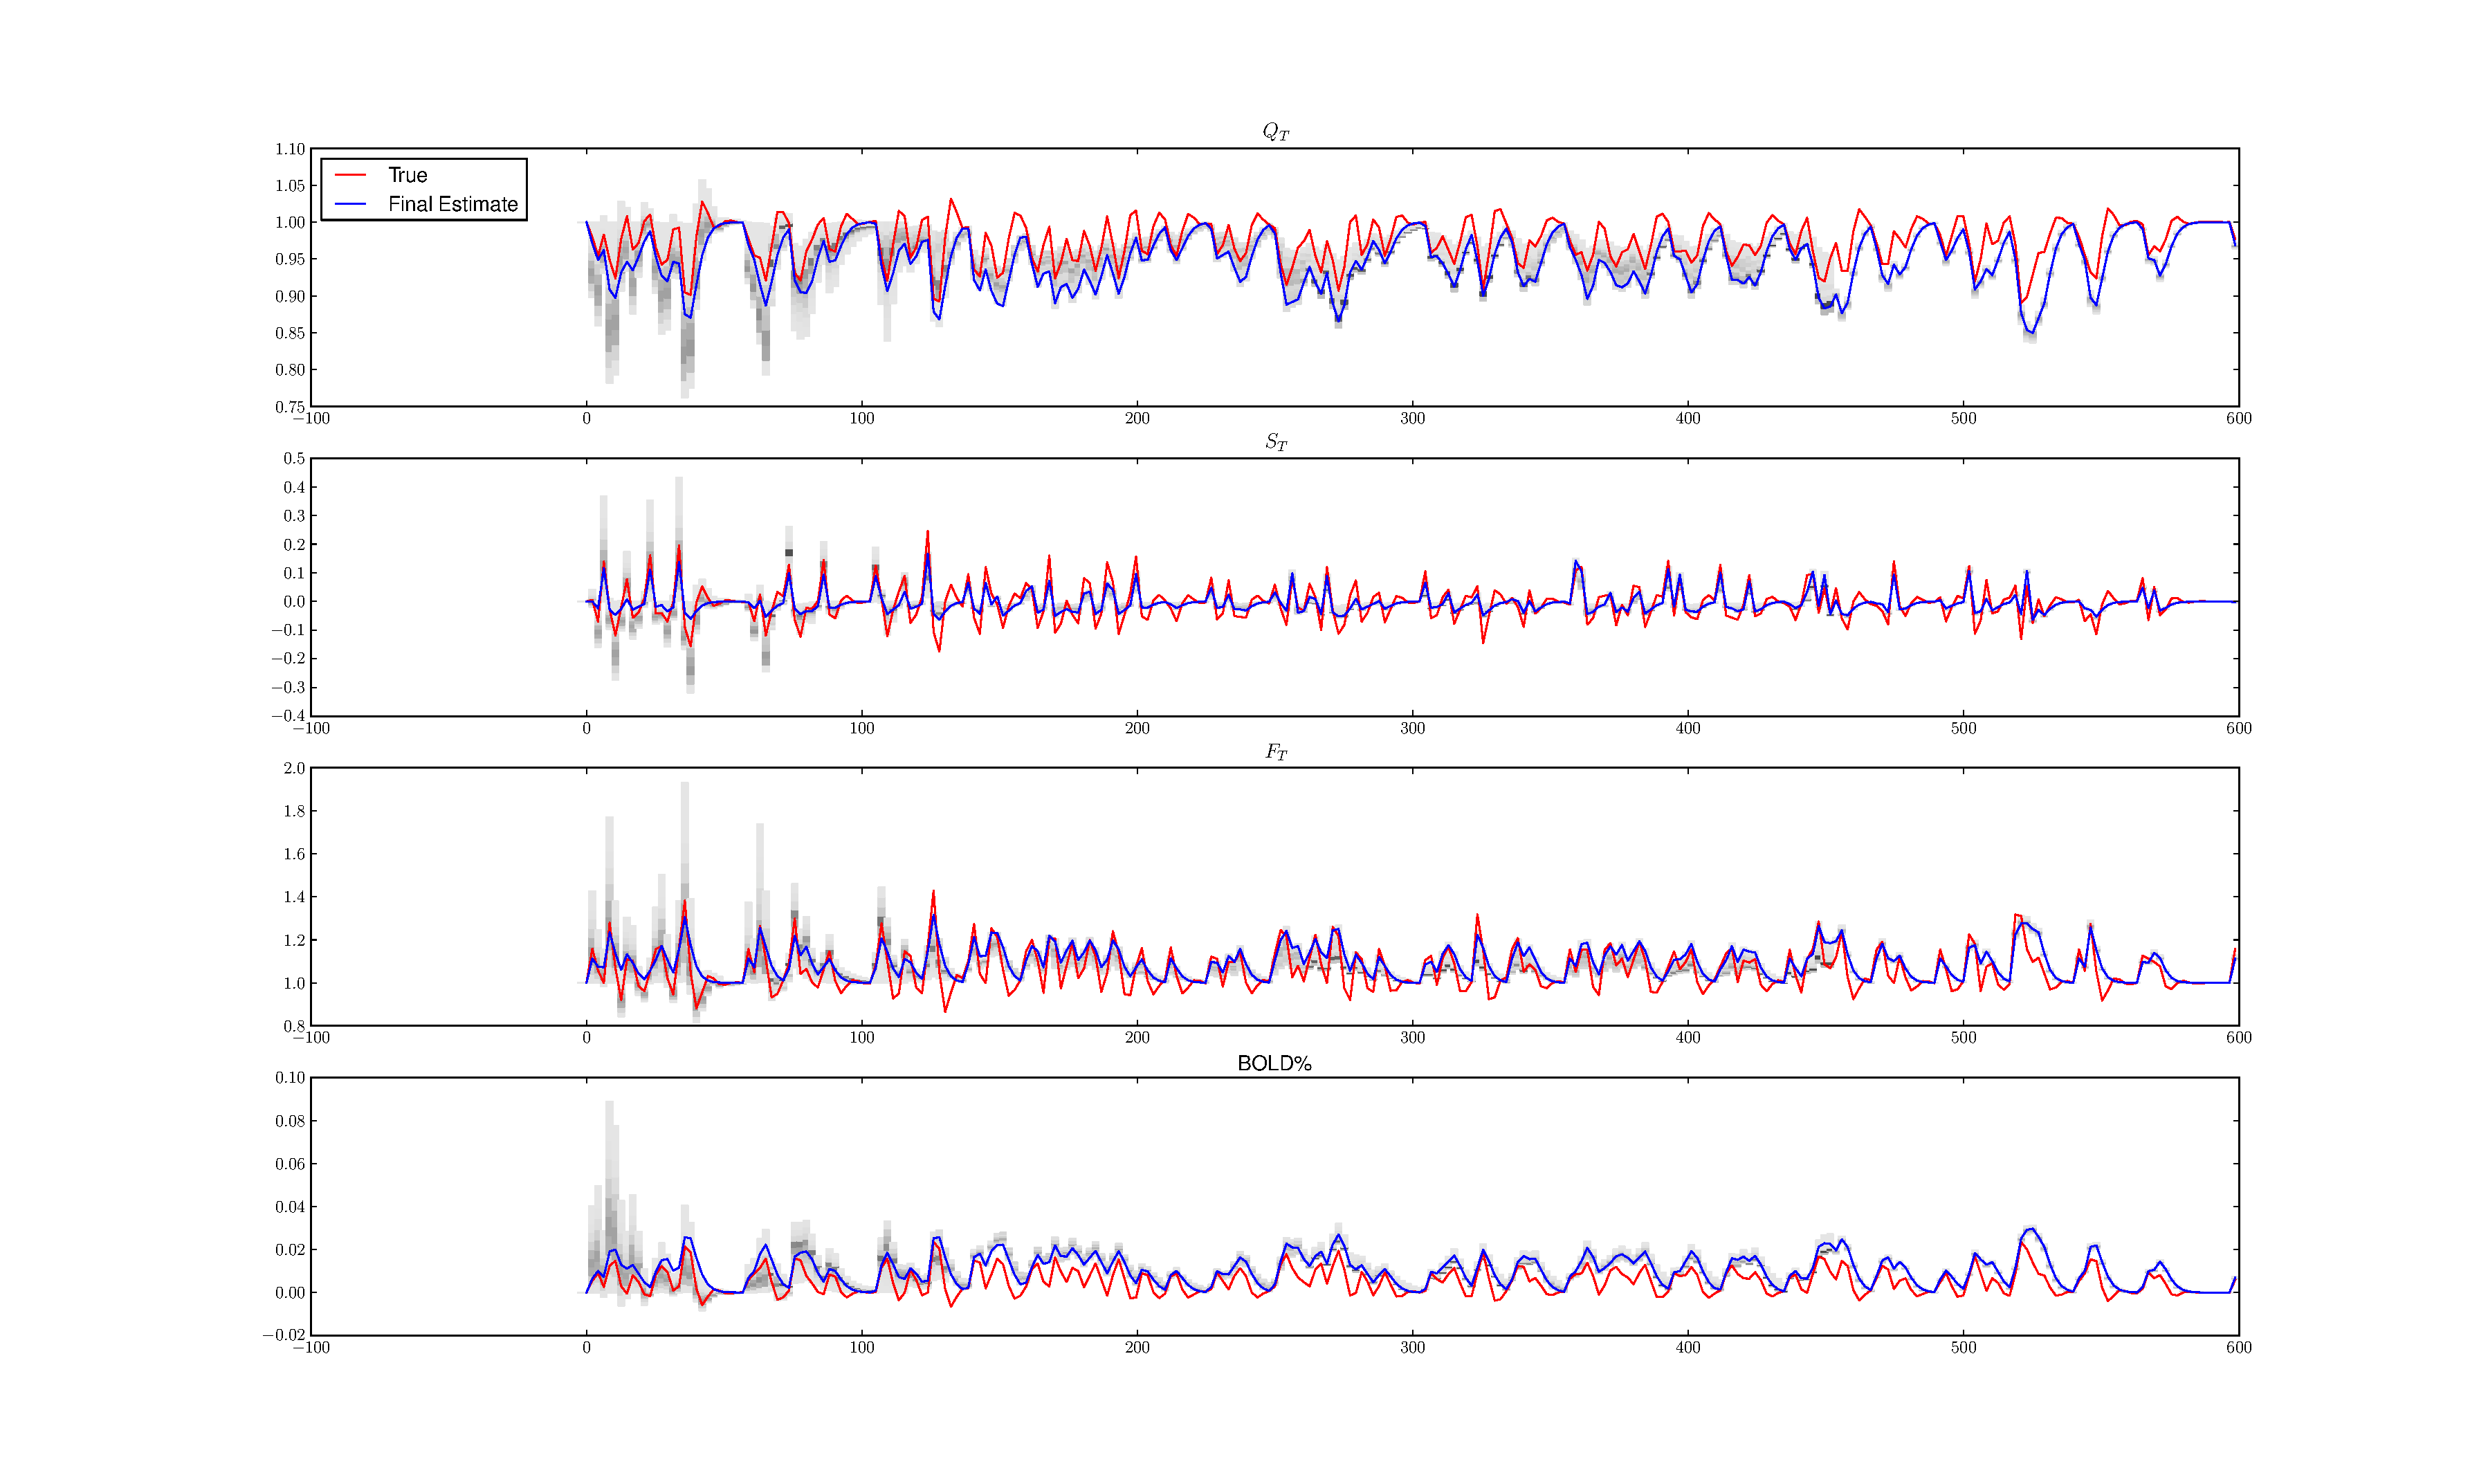
\includegraphics[clip=true,trim=6cm 2cm 6cm 3cm, width=14cm]{images/highnoise_run6_3}}
\caption{Converging histogram for parameters during run 2, as in \autoref{fig:NoiseComparisonJustTwo}.}
\label{fig:ConvergenceRuns2}
\end{figure}

There are a number of interesting convergence properties of the
particle filter when more noise is present, as both \autoref{fig:ConvergenceRuns1} and
\autoref{fig:ConvergenceRuns2} show. The particle filter seems to converge
significantly faster; as points tend to be further out on the weighting function. This
also causes significantly more resampling which is the explanation for the percieved
jumps in resolution that occur from time to time. Here it is clear that the mode and
the mean will not be substantially different. Because of the increased noise, its likely
that the weighting function is not sufficiently wide to account for the measurement noise.

The parameters arrived at for all ten filter runs are shown in \autoref{tab:HighNoiseResults}.
Clearly the additional noise have resulted in much more sporadic results. This is often the 
result when the particle filter converges too fast, a result of the weighting functions' variance
being significantly smaller than the measurement noise ($.005$ vs. $.01$). The square-root
MSE certainly suffers due to this effect.

%NO SIGNAL, LOW NOISE
\subsection{Pure-Noise, low magnitude}
\label{sec:PureNoiseLowMag}
The two final single-voxel tests force the particle filter to attempt to "learn" a noise-only
time series. In the first test the noise used will be the same as that from the \autoref{sec:HighNoise},
$\sigma_x = .01, \sigma_y = .005$. The parameters will be set the same as well, but the
stimulus/input will be set to 0 the entire time. In effect it is a region of the brain for
which no visual stimulus induces activity. For the particle filter, on the other hand,
the stimulus will be left as in the previous two sections. The question then is how the
particle filter will respond to signal that does not correlate with the input, and how
the output may be differentiated from a time series that does. The time series'
are shown in \autoref{fig:NoiseOnly}, the preprocessed versions are shown in \autoref{fig:PreprocessedNoiseOnly}.
The line fits are shown in \autoref{fig:fits_noiseonly}. 


\begin{figure}[H]
\centering
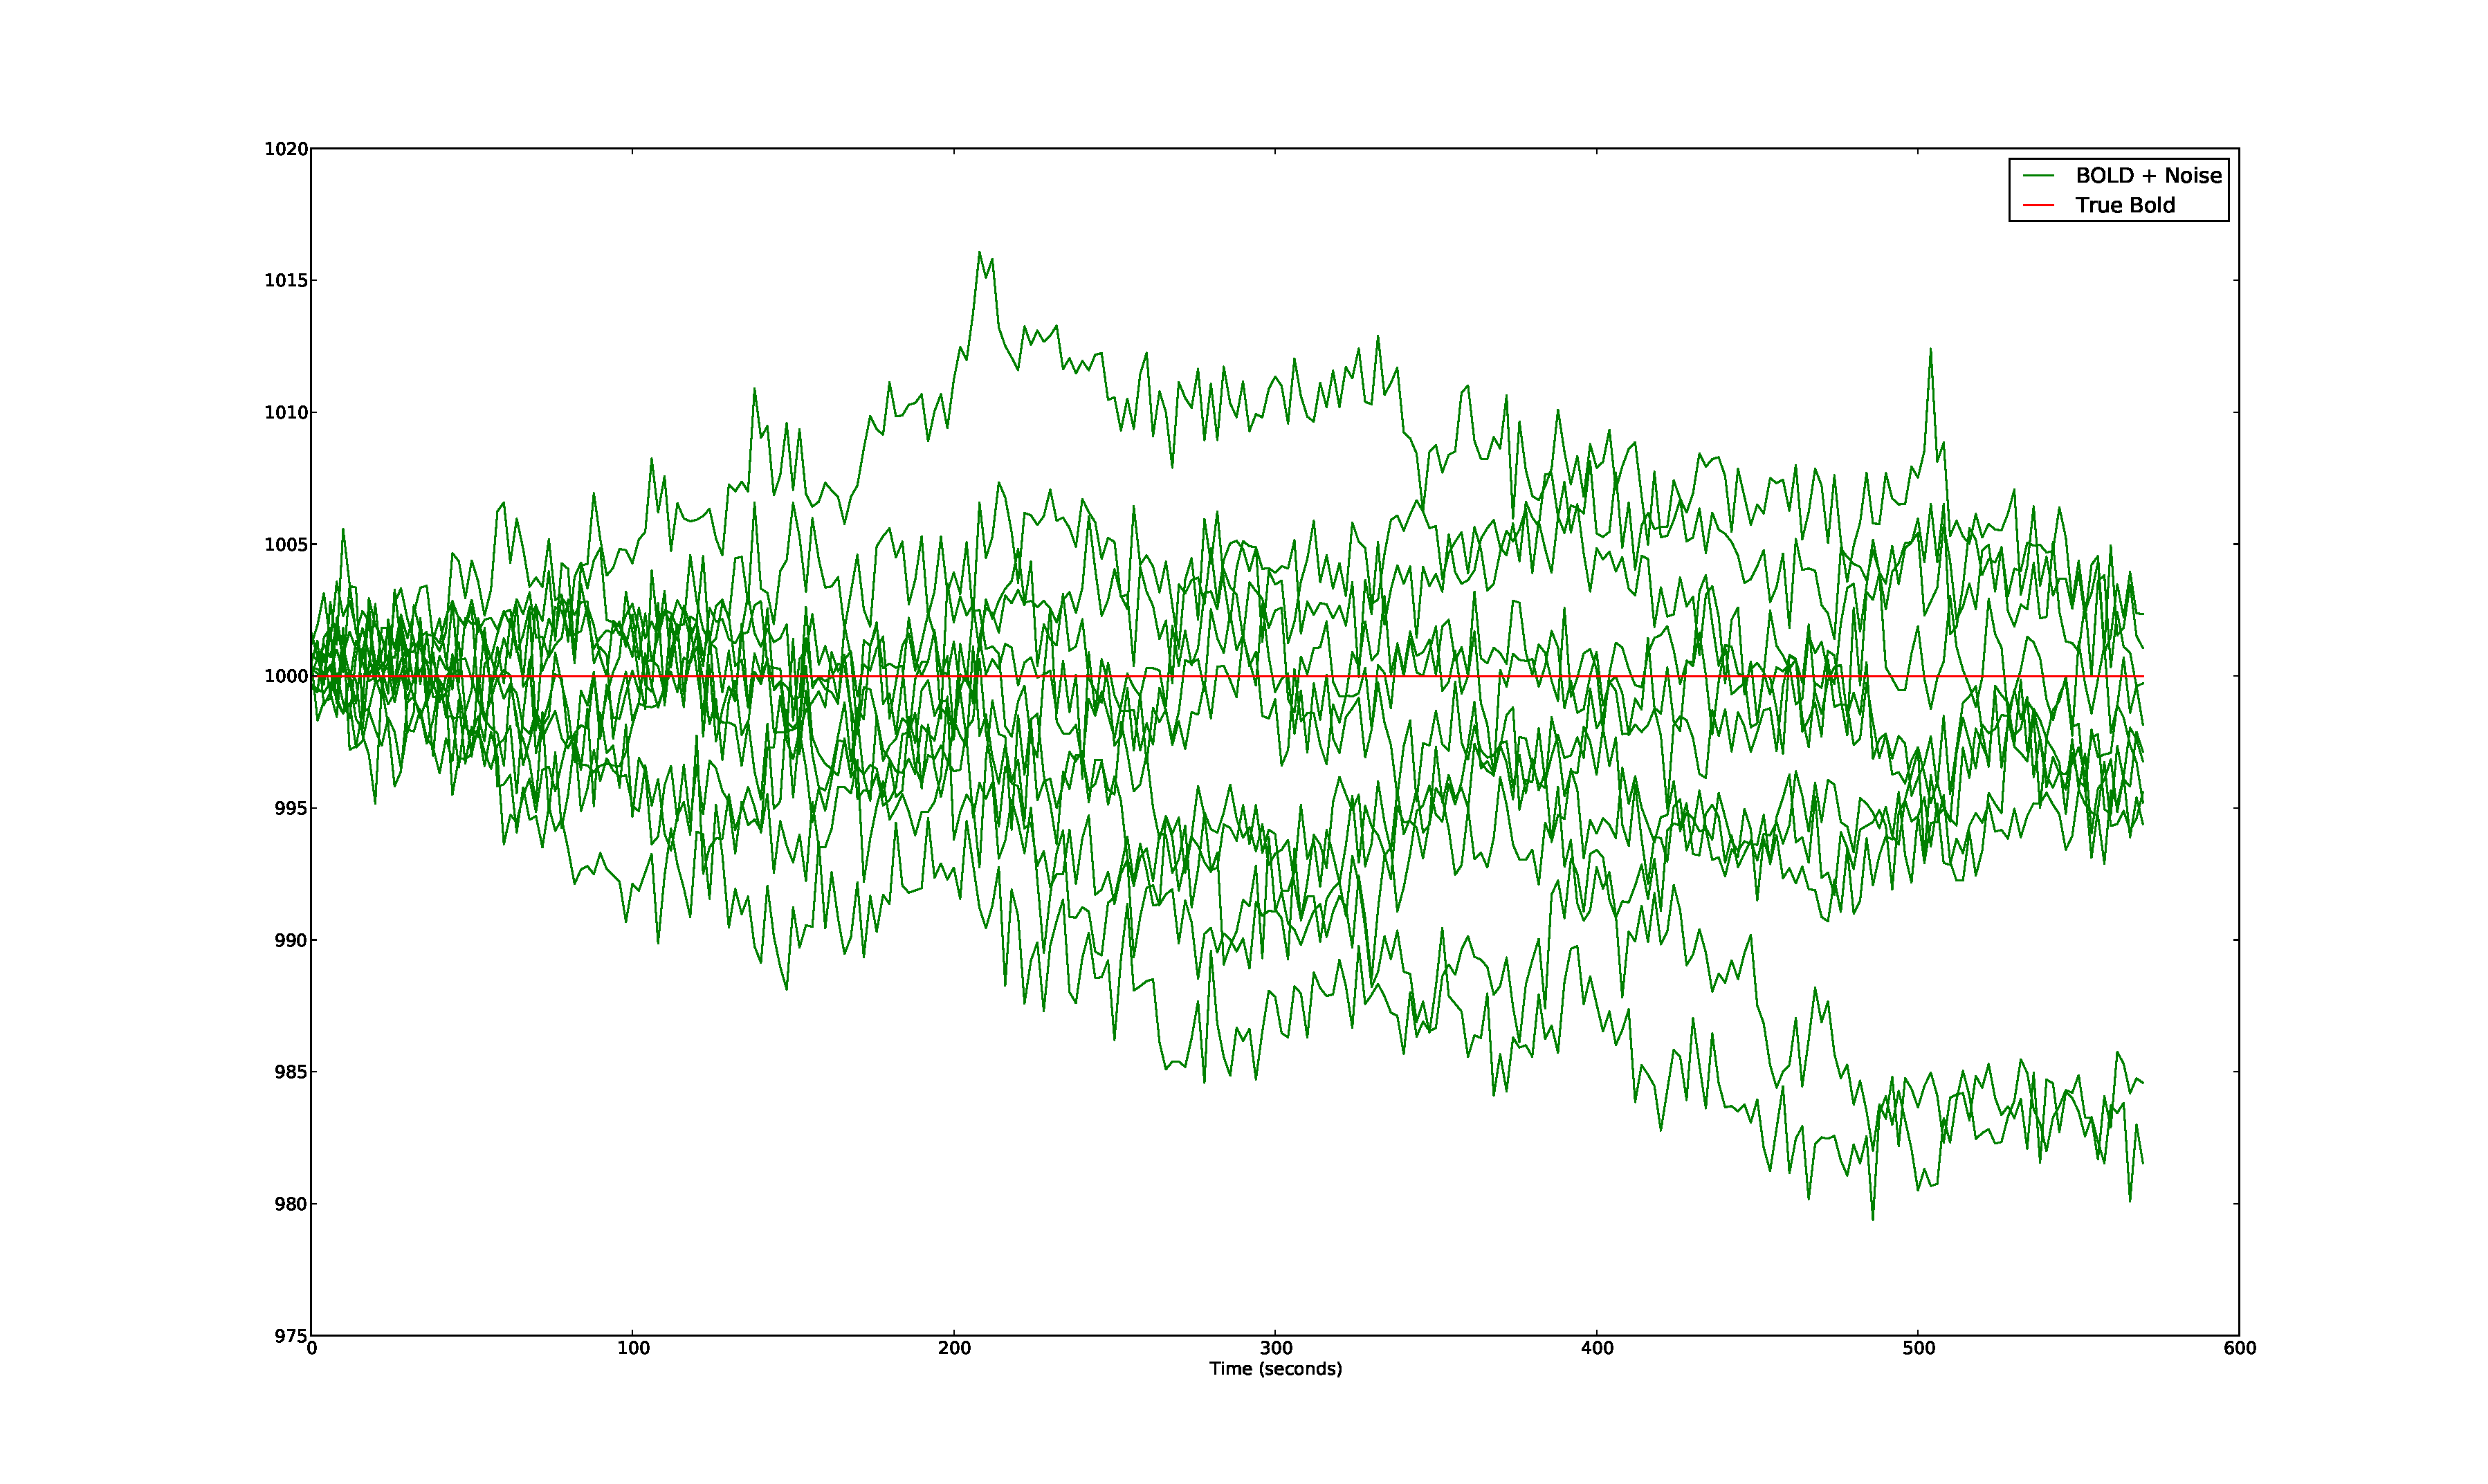
\includegraphics[clip=true,trim=6cm 3cm 6cm 3cm,height=9cm]{images/realization_noiseonly}
\caption{Time-series lacking any real signal. With, $\sigma_x = .01, \sigma_y=.005$}
\label{fig:NoiseOnly}
\end{figure}

\begin{figure}[H]
\centering
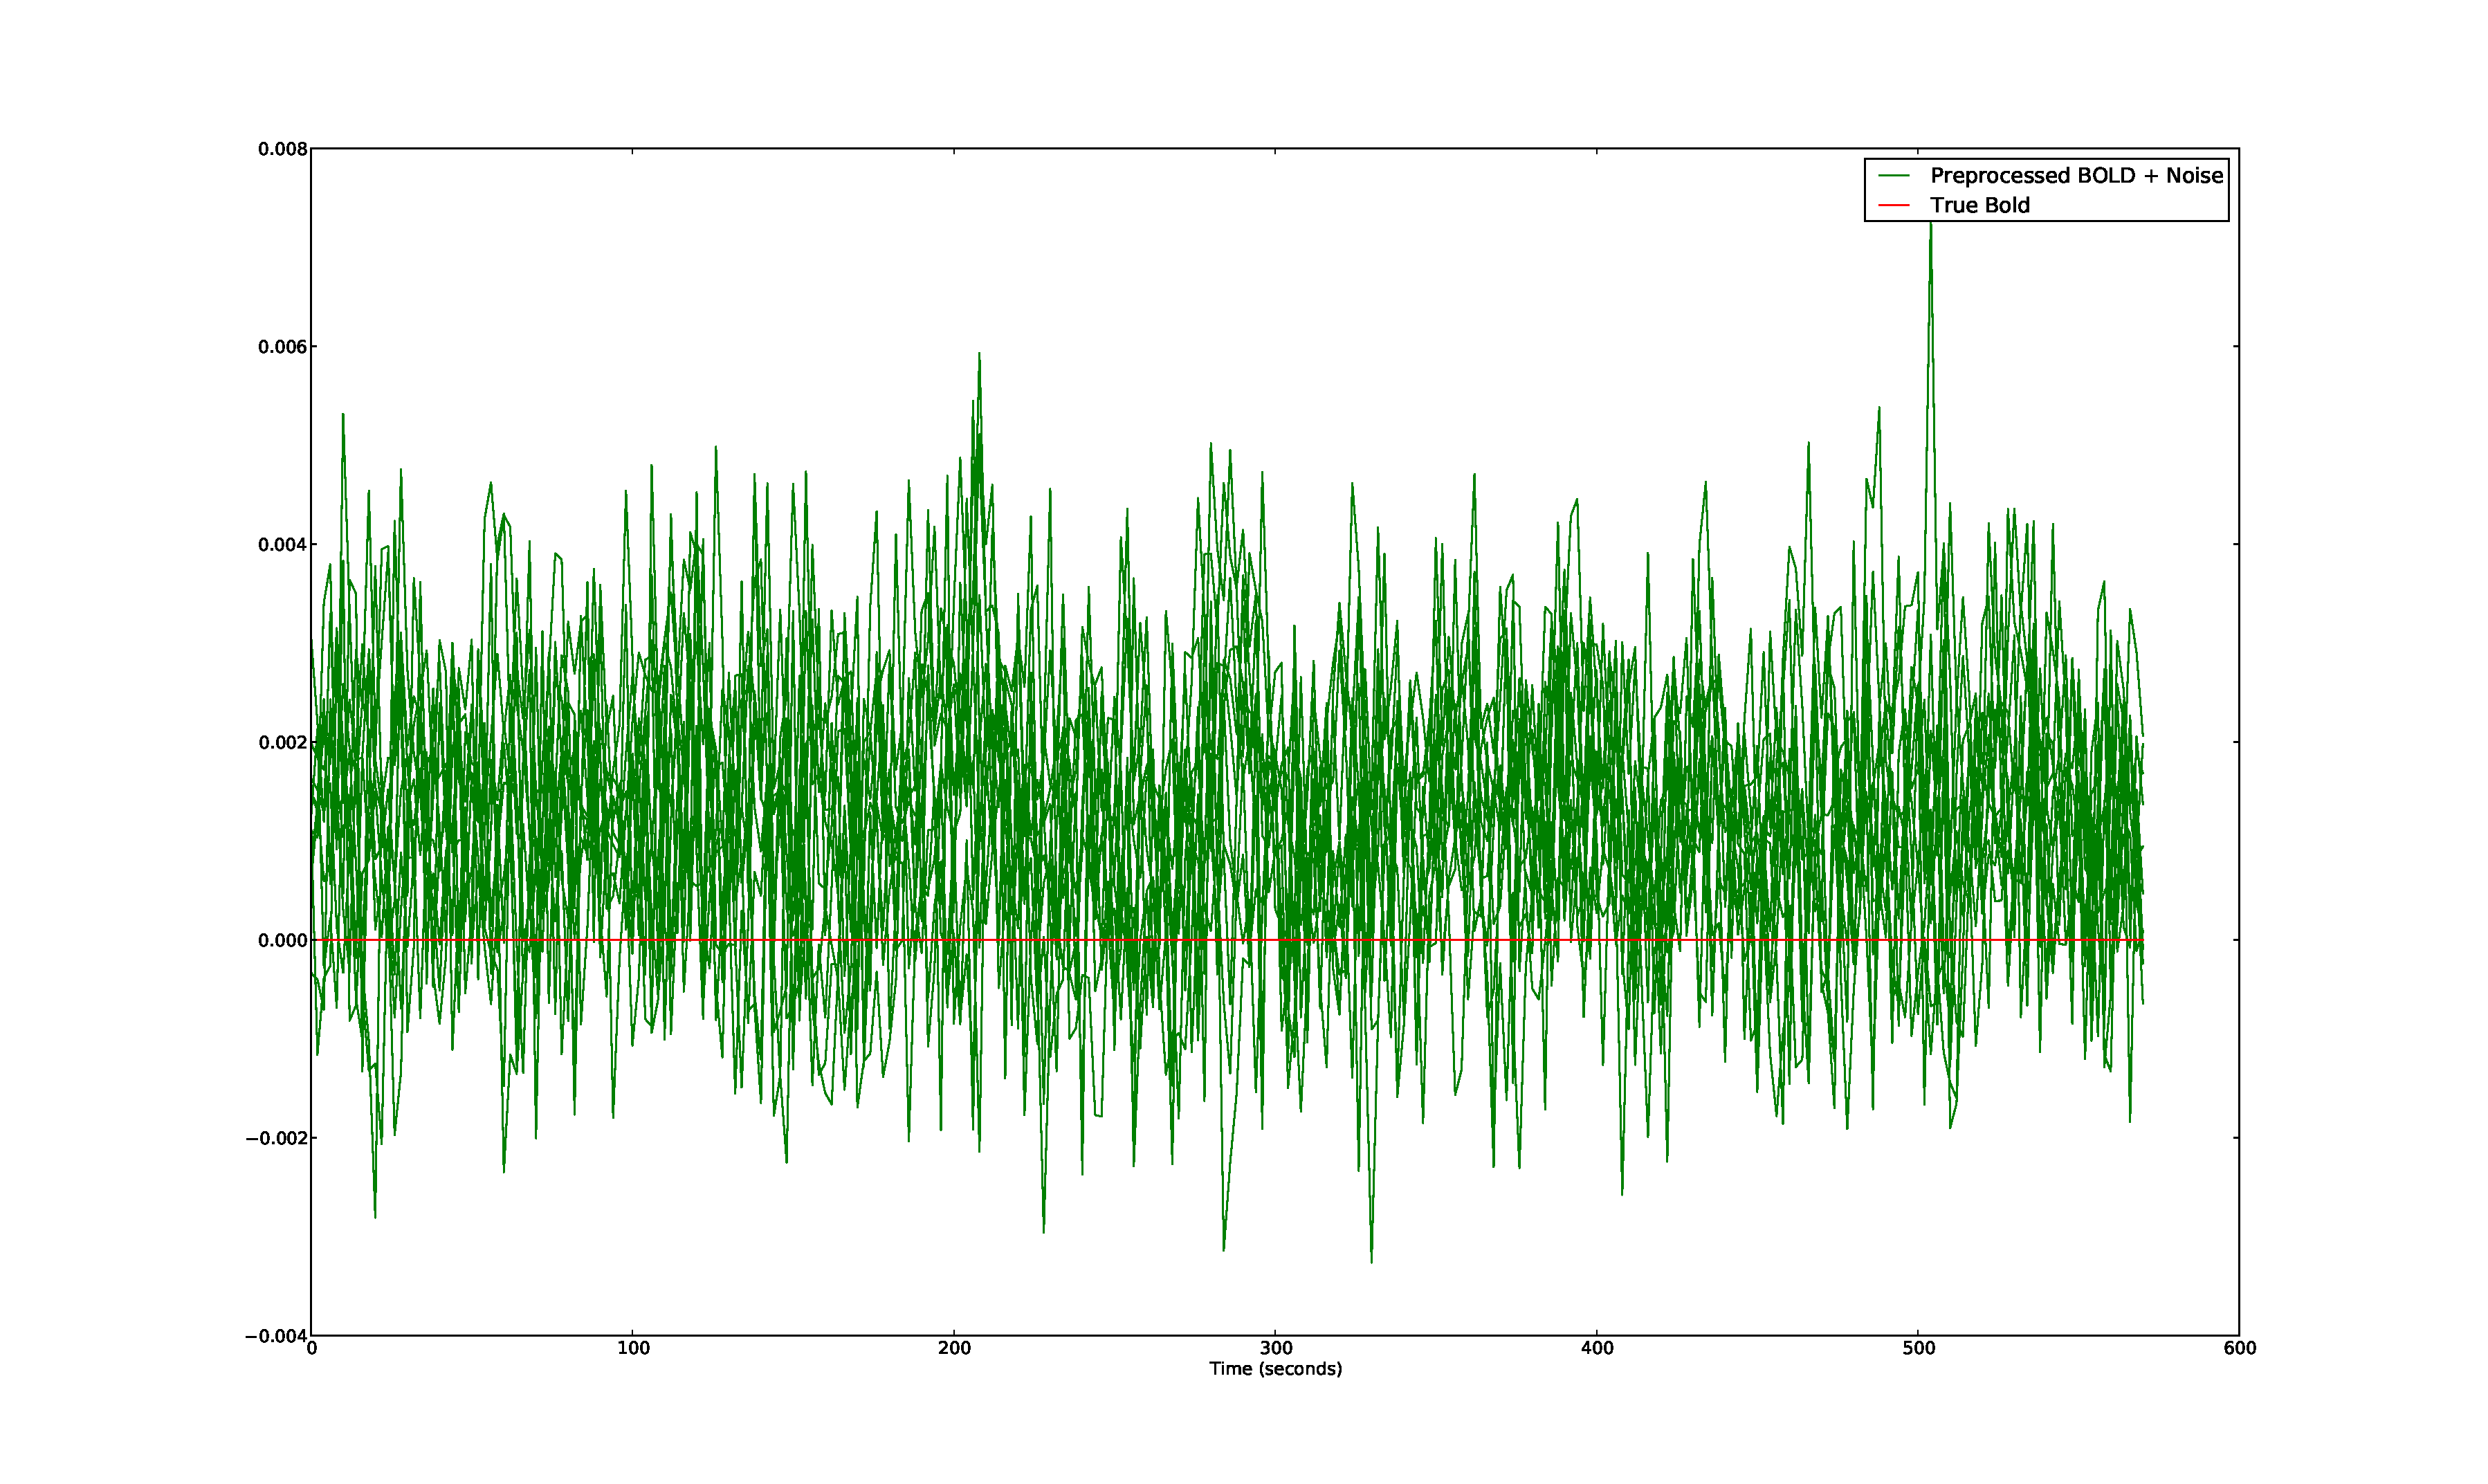
\includegraphics[clip=true,trim=6cm 3cm 6cm 3cm,height=9cm]{images/preprocessed_noiseonly}
\caption{A comparison of the preprocessed signals for the signal-free case. (
$\sigma_y = .01, \sigma_x = .005$)}
\label{fig:PreprocessedNoiseOnly}
\end{figure}

\begin{table}[t]
\centering
\begin{tabular}{|c | c | c | c | c | c | c | c | c |}
\hline 
$\tau_0$ & $\alpha$ & $E_0$    & $V_0$    & $\tau_s$ & $\tau_f$ & $\epsilon$  &  $\sqrt{MSR}$   \\
\hline 
1.0324 & 0.33211 & 0.34058 & 0.03012 & 1.40665 & 2.52079 & 0.5311 & \\
 0.98189 & 0.33047 & 0.3386 & 0.03014 & 1.45707 & 2.47232 & 0.45049 & 0.00158551 \\
 1.0429 & 0.33224 & 0.34124 & 0.02946 & 1.4618 & 2.49245 & 0.43012 &  0.00165055 \\
 1.02054 & 0.3321 & 0.33484 & 0.02586 & 1.45848 & 2.48741 & 0.4193 &  0.00150604 \\
 1.0565 & 0.33405 & 0.33758 & 0.02791 & 1.43784 & 2.52545 & 0.47517 & 0.00151513 \\
 1.01867 & 0.33528 & 0.33918 & 0.02782 & 1.48345 & 2.49605 & 0.44209 &0.00155645 \\
 1.051 & 0.33038 & 0.33837 & 0.02985 & 1.47651 & 2.48621 & 0.42719 &  0.00158526 \\
 1.00281 & 0.32929 & 0.33988 & 0.0298 & 1.43519 & 2.49256 & 0.48899 & 0.00164299 \\
 1.00893 & 0.33273 & 0.33982 & 0.0289 & 1.42903 & 2.49754 & 0.45688 & 0.0016793  \\
 1.01289 & 0.33275 & 0.3376 & 0.02997 & 1.41188 & 2.49881 & 0.50628 & 0.00182622 \\
 1.10247 & 0.33371 & 0.3419 & 0.02939 & 1.43774 & 2.53384 & 0.44079 & 0.00195009 \\
\hline                                                                
1.03009 & 0.33228 & 0.33905 & 0.02902 & 1.44506 & 2.50031 & 0.46076 & 0.00165129 \\
\hline 
\end{tabular}
\caption{Estimated Parameters on 11 different runs with low noise and no signal present.}
\label{tab:NoiseOnlyResults} 
\end{table}

\begin{figure}[H]
\centering
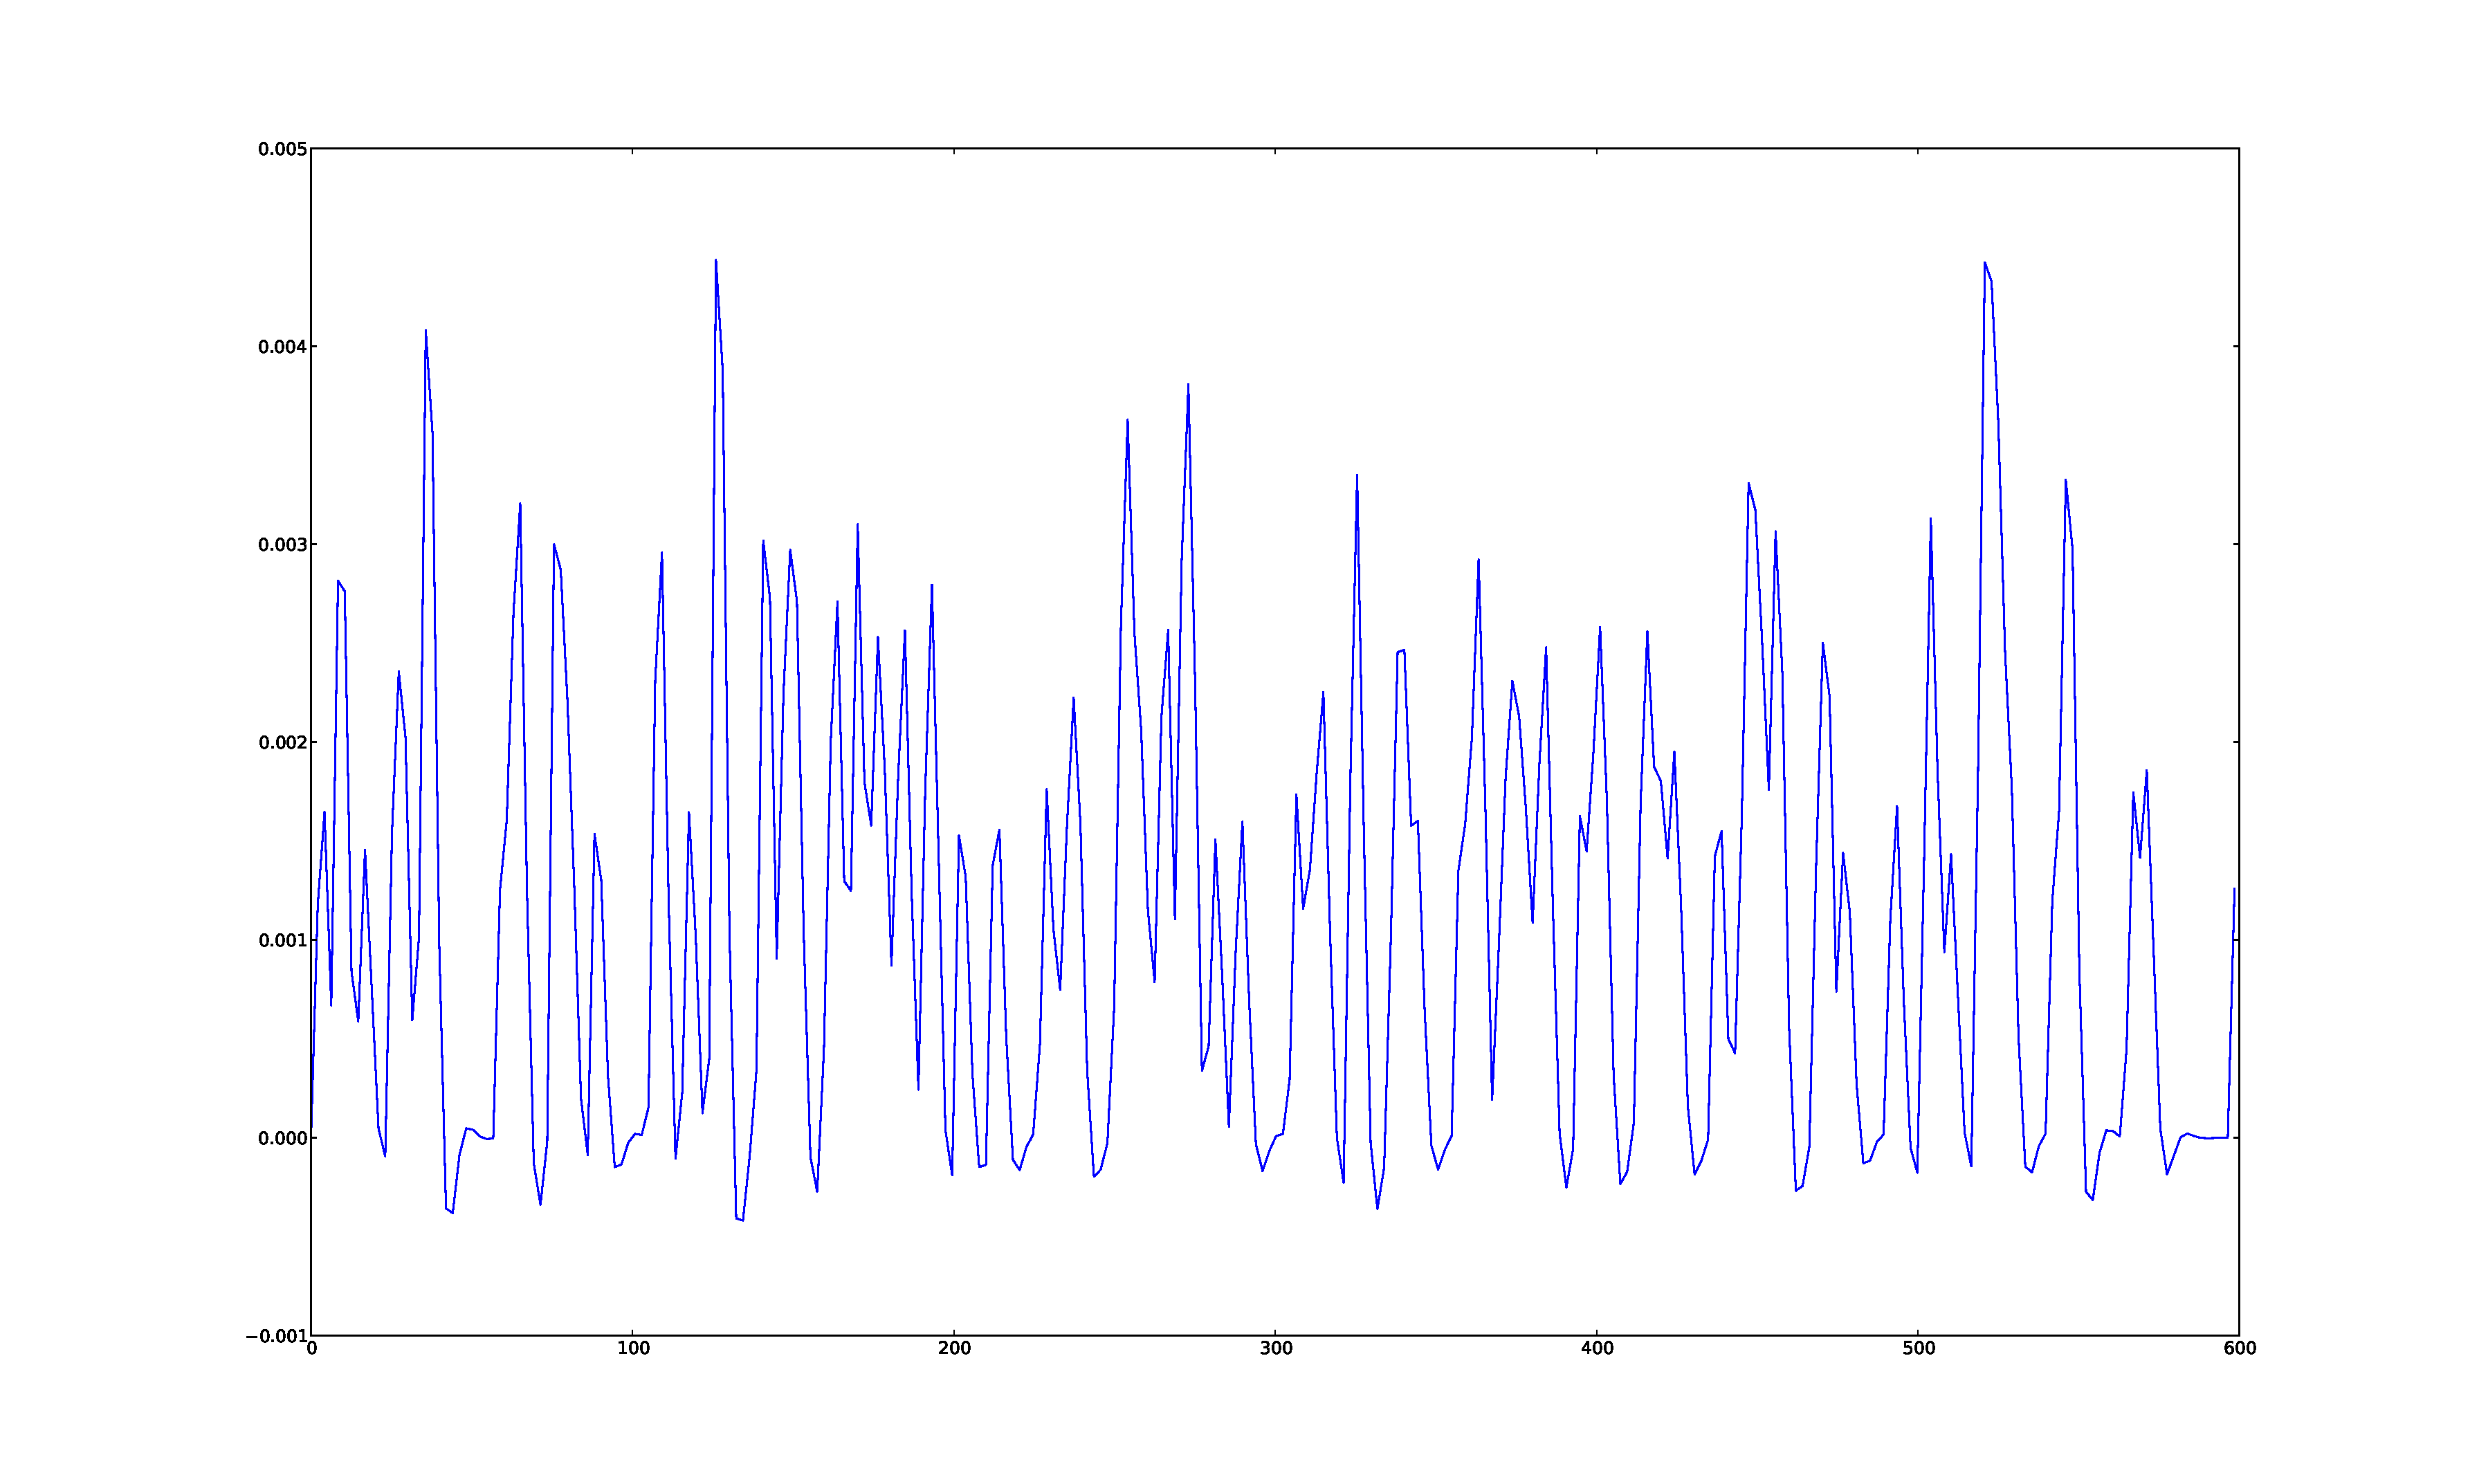
\includegraphics[clip=true,trim=6cm 3cm 6cm 3cm,height=9cm]{images/fits_noiseonly}
\caption{Fits to the non-active, low noise signal. Note that the line is thick because all
the fits overlap. This is all 11 fitted lines.}
\label{fig:fits_noiseonly}
\end{figure}

\begin{figure}[H]
\centering
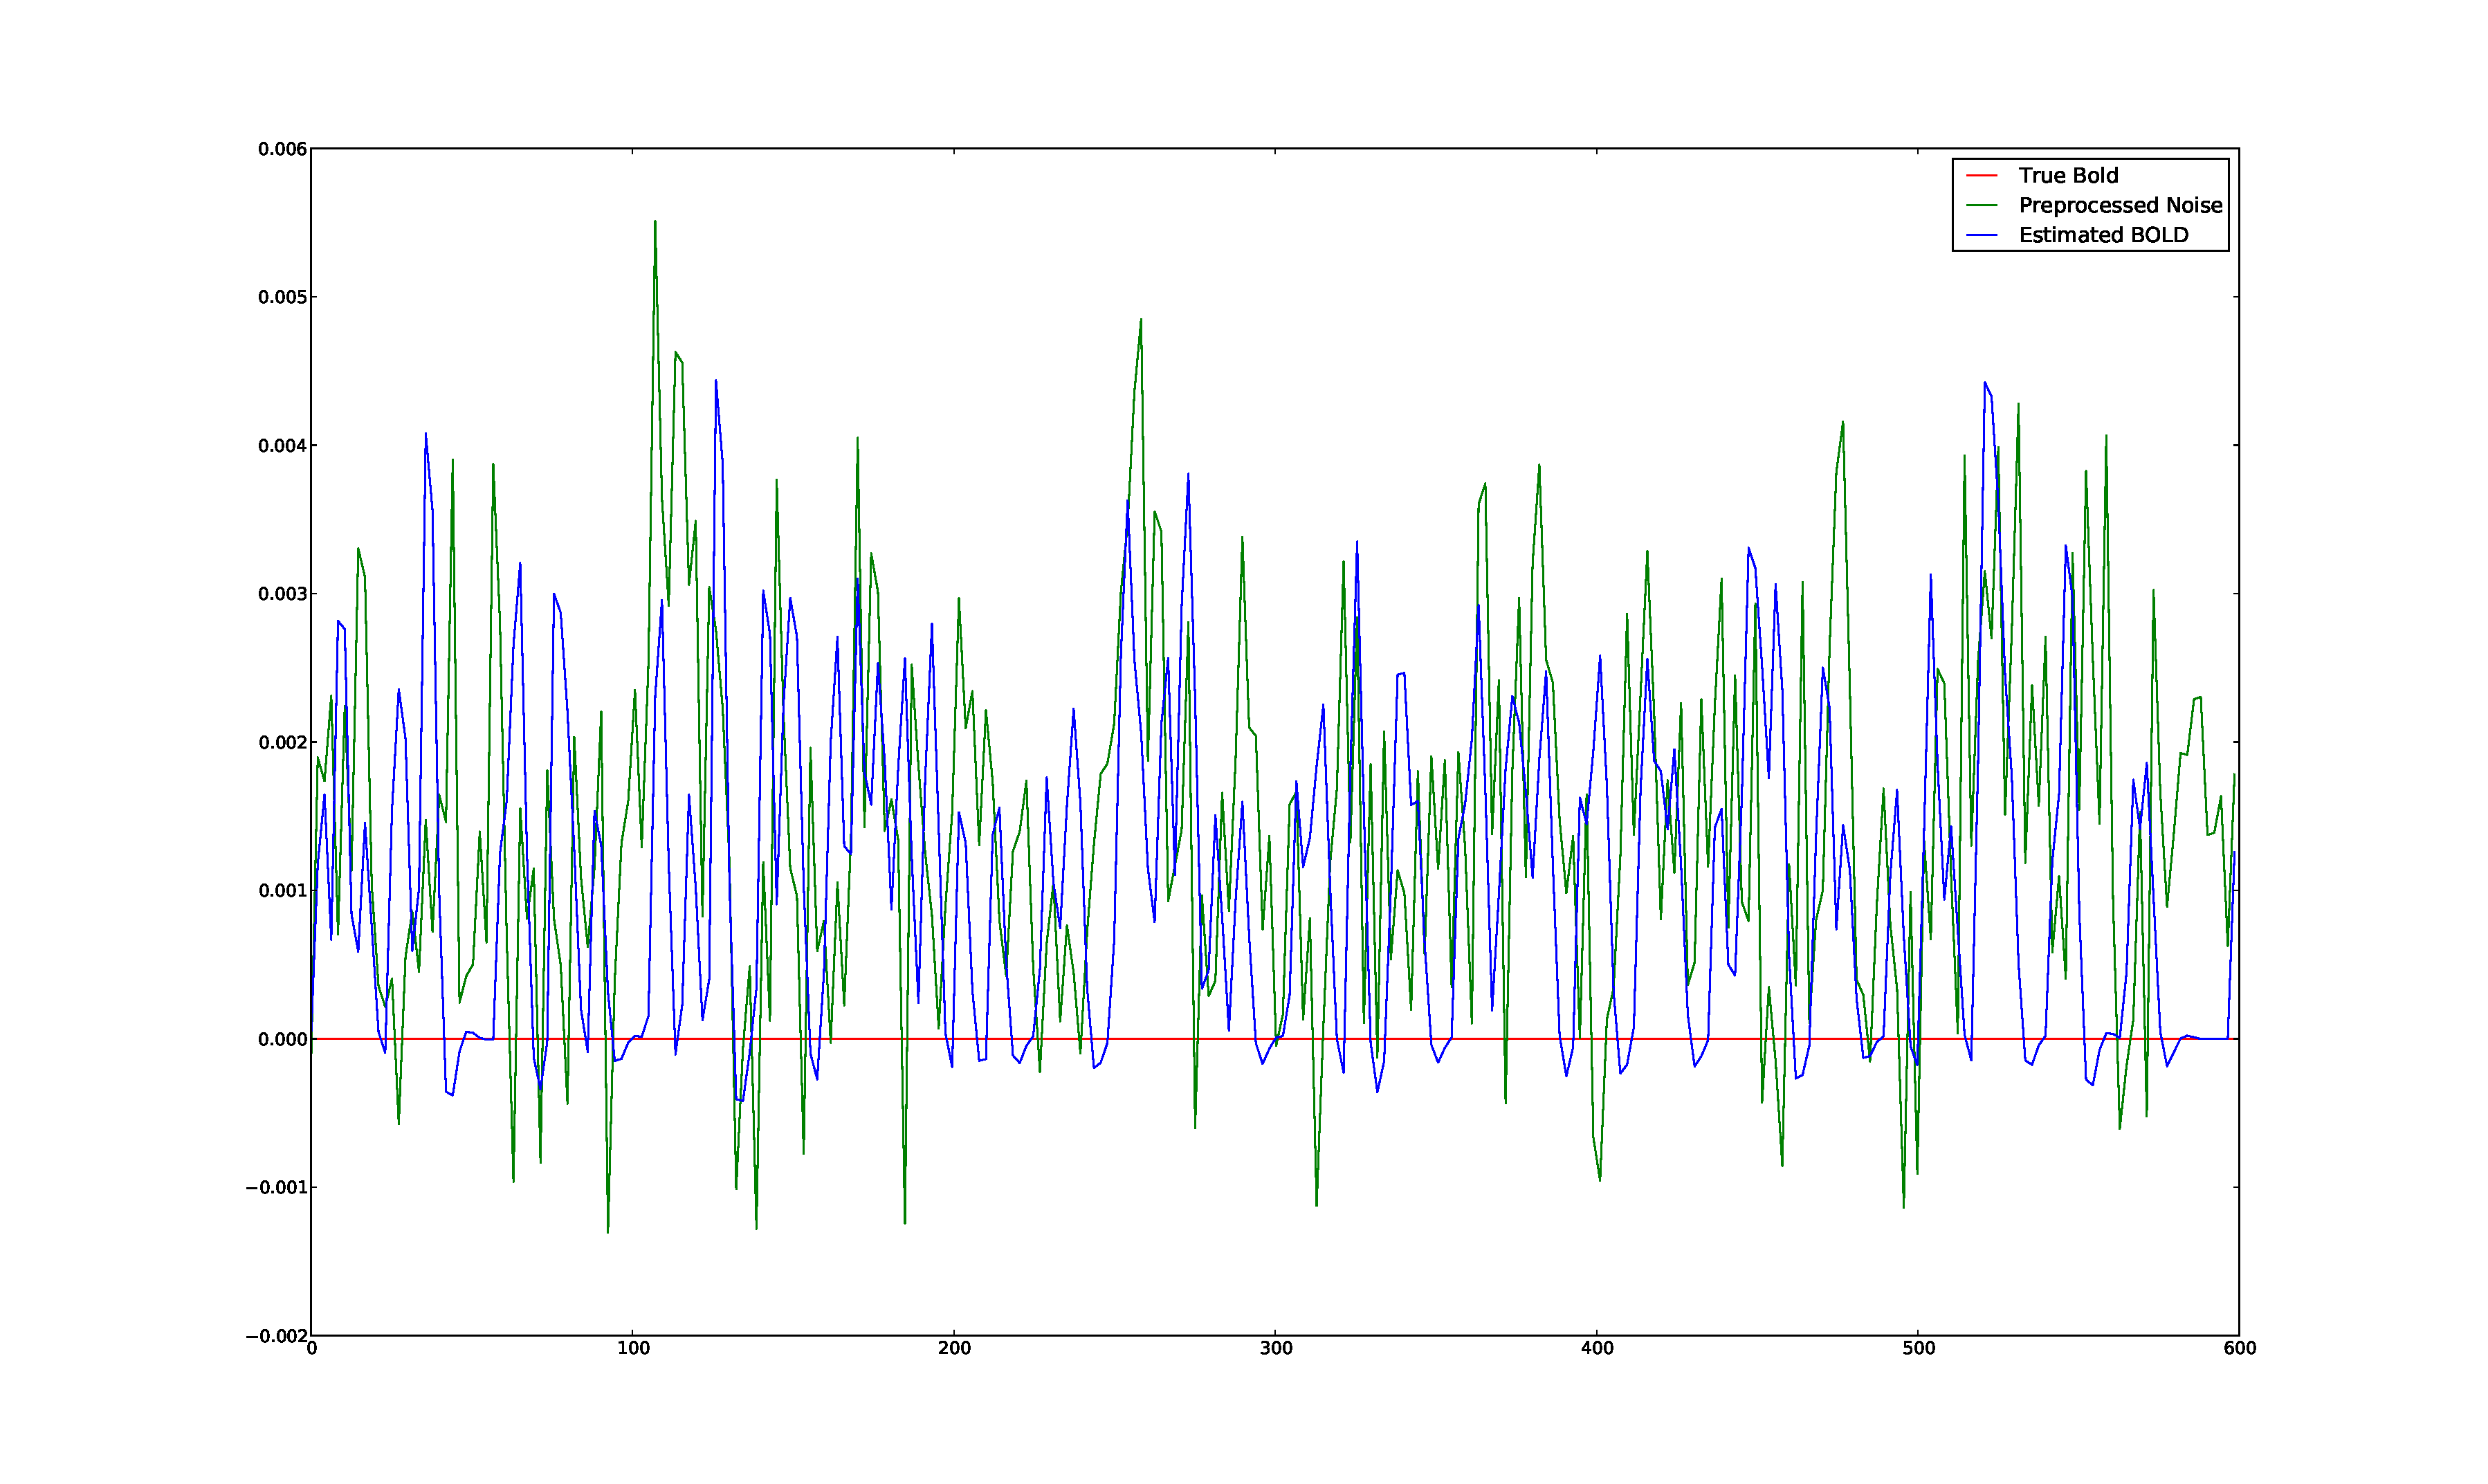
\includegraphics[clip=true,trim=6cm 3cm 6cm 3cm,height=9cm]{images/justnoise_fit_0}
\caption{Fit from a single particle filter run, with the noise input. }
\label{fig:justnoise_fit_0}
\end{figure} %uses allnoise/ALLNOISE-0-w0

\begin{figure}[H]
\centering
\subfigure[$\tau_0$, $\alpha$, $E_0$, $V_0$]
{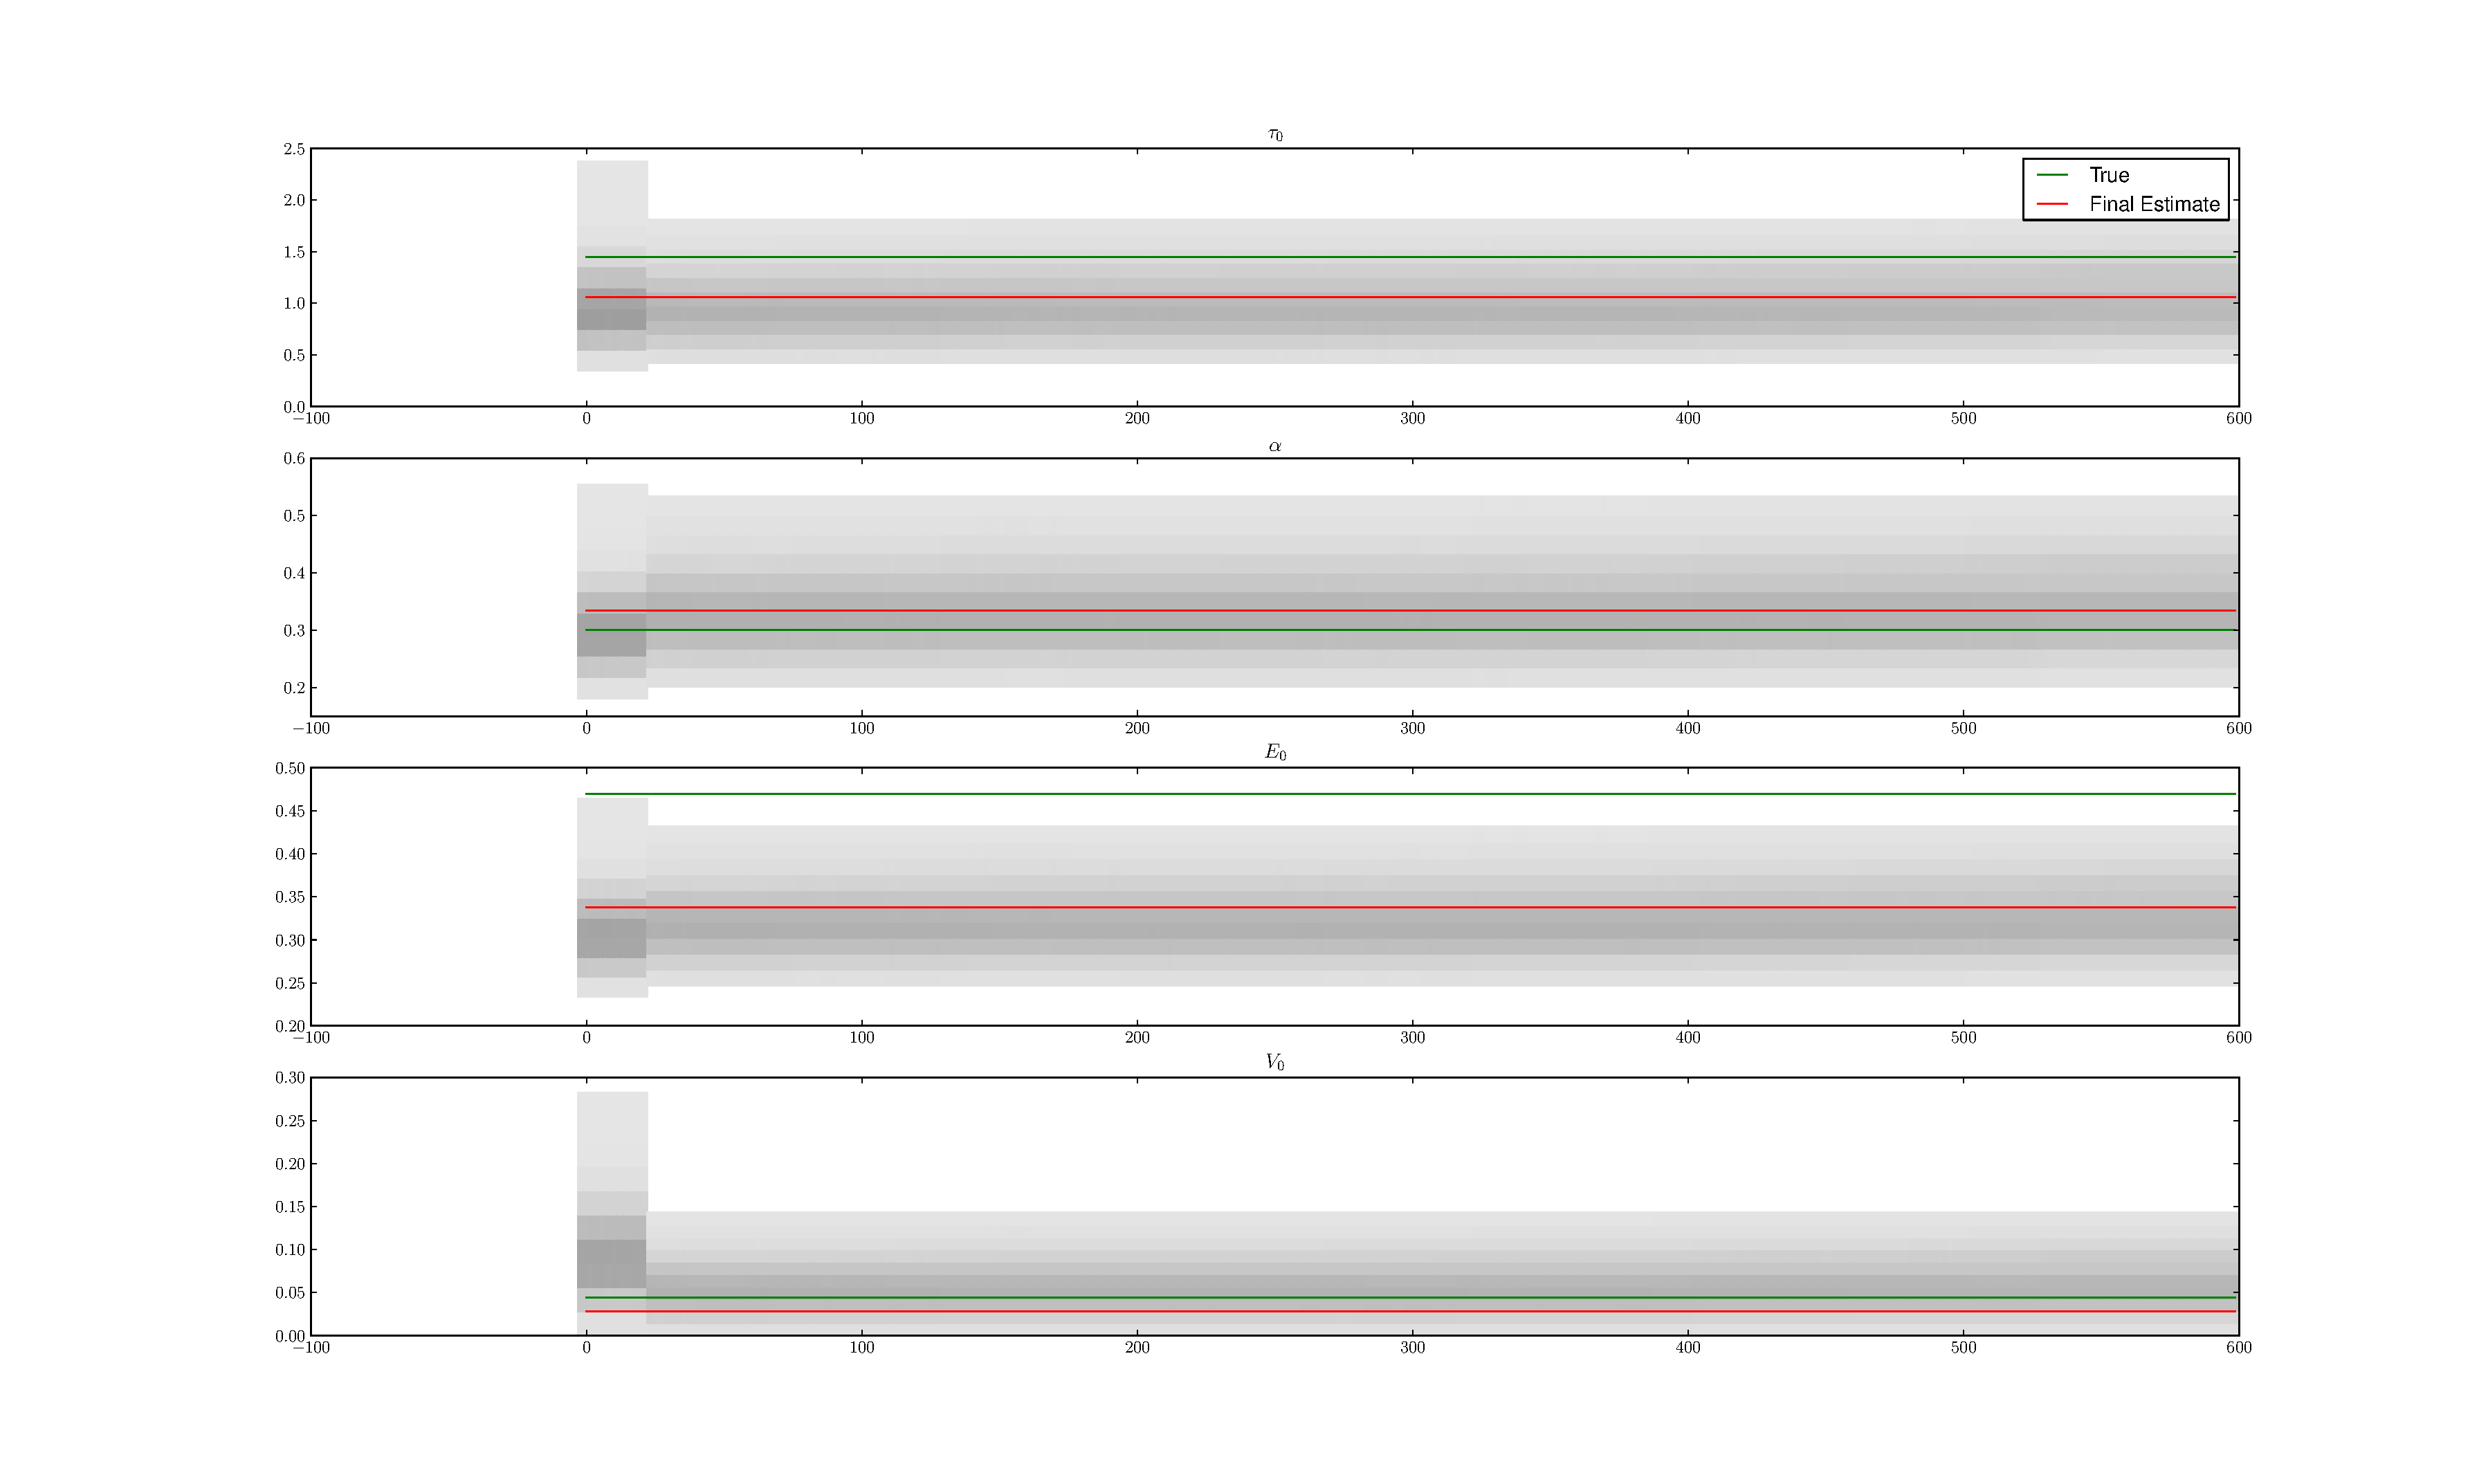
\includegraphics[clip=true,trim=6cm 2cm 6cm 3cm, height=9cm]{images/justnoise_hist_1}}\\
\end{figure}

\begin{figure}[H]
\centering
\subfigure[$\tau_s$, $\tau_f$, $\epsilon$, $V$] 
{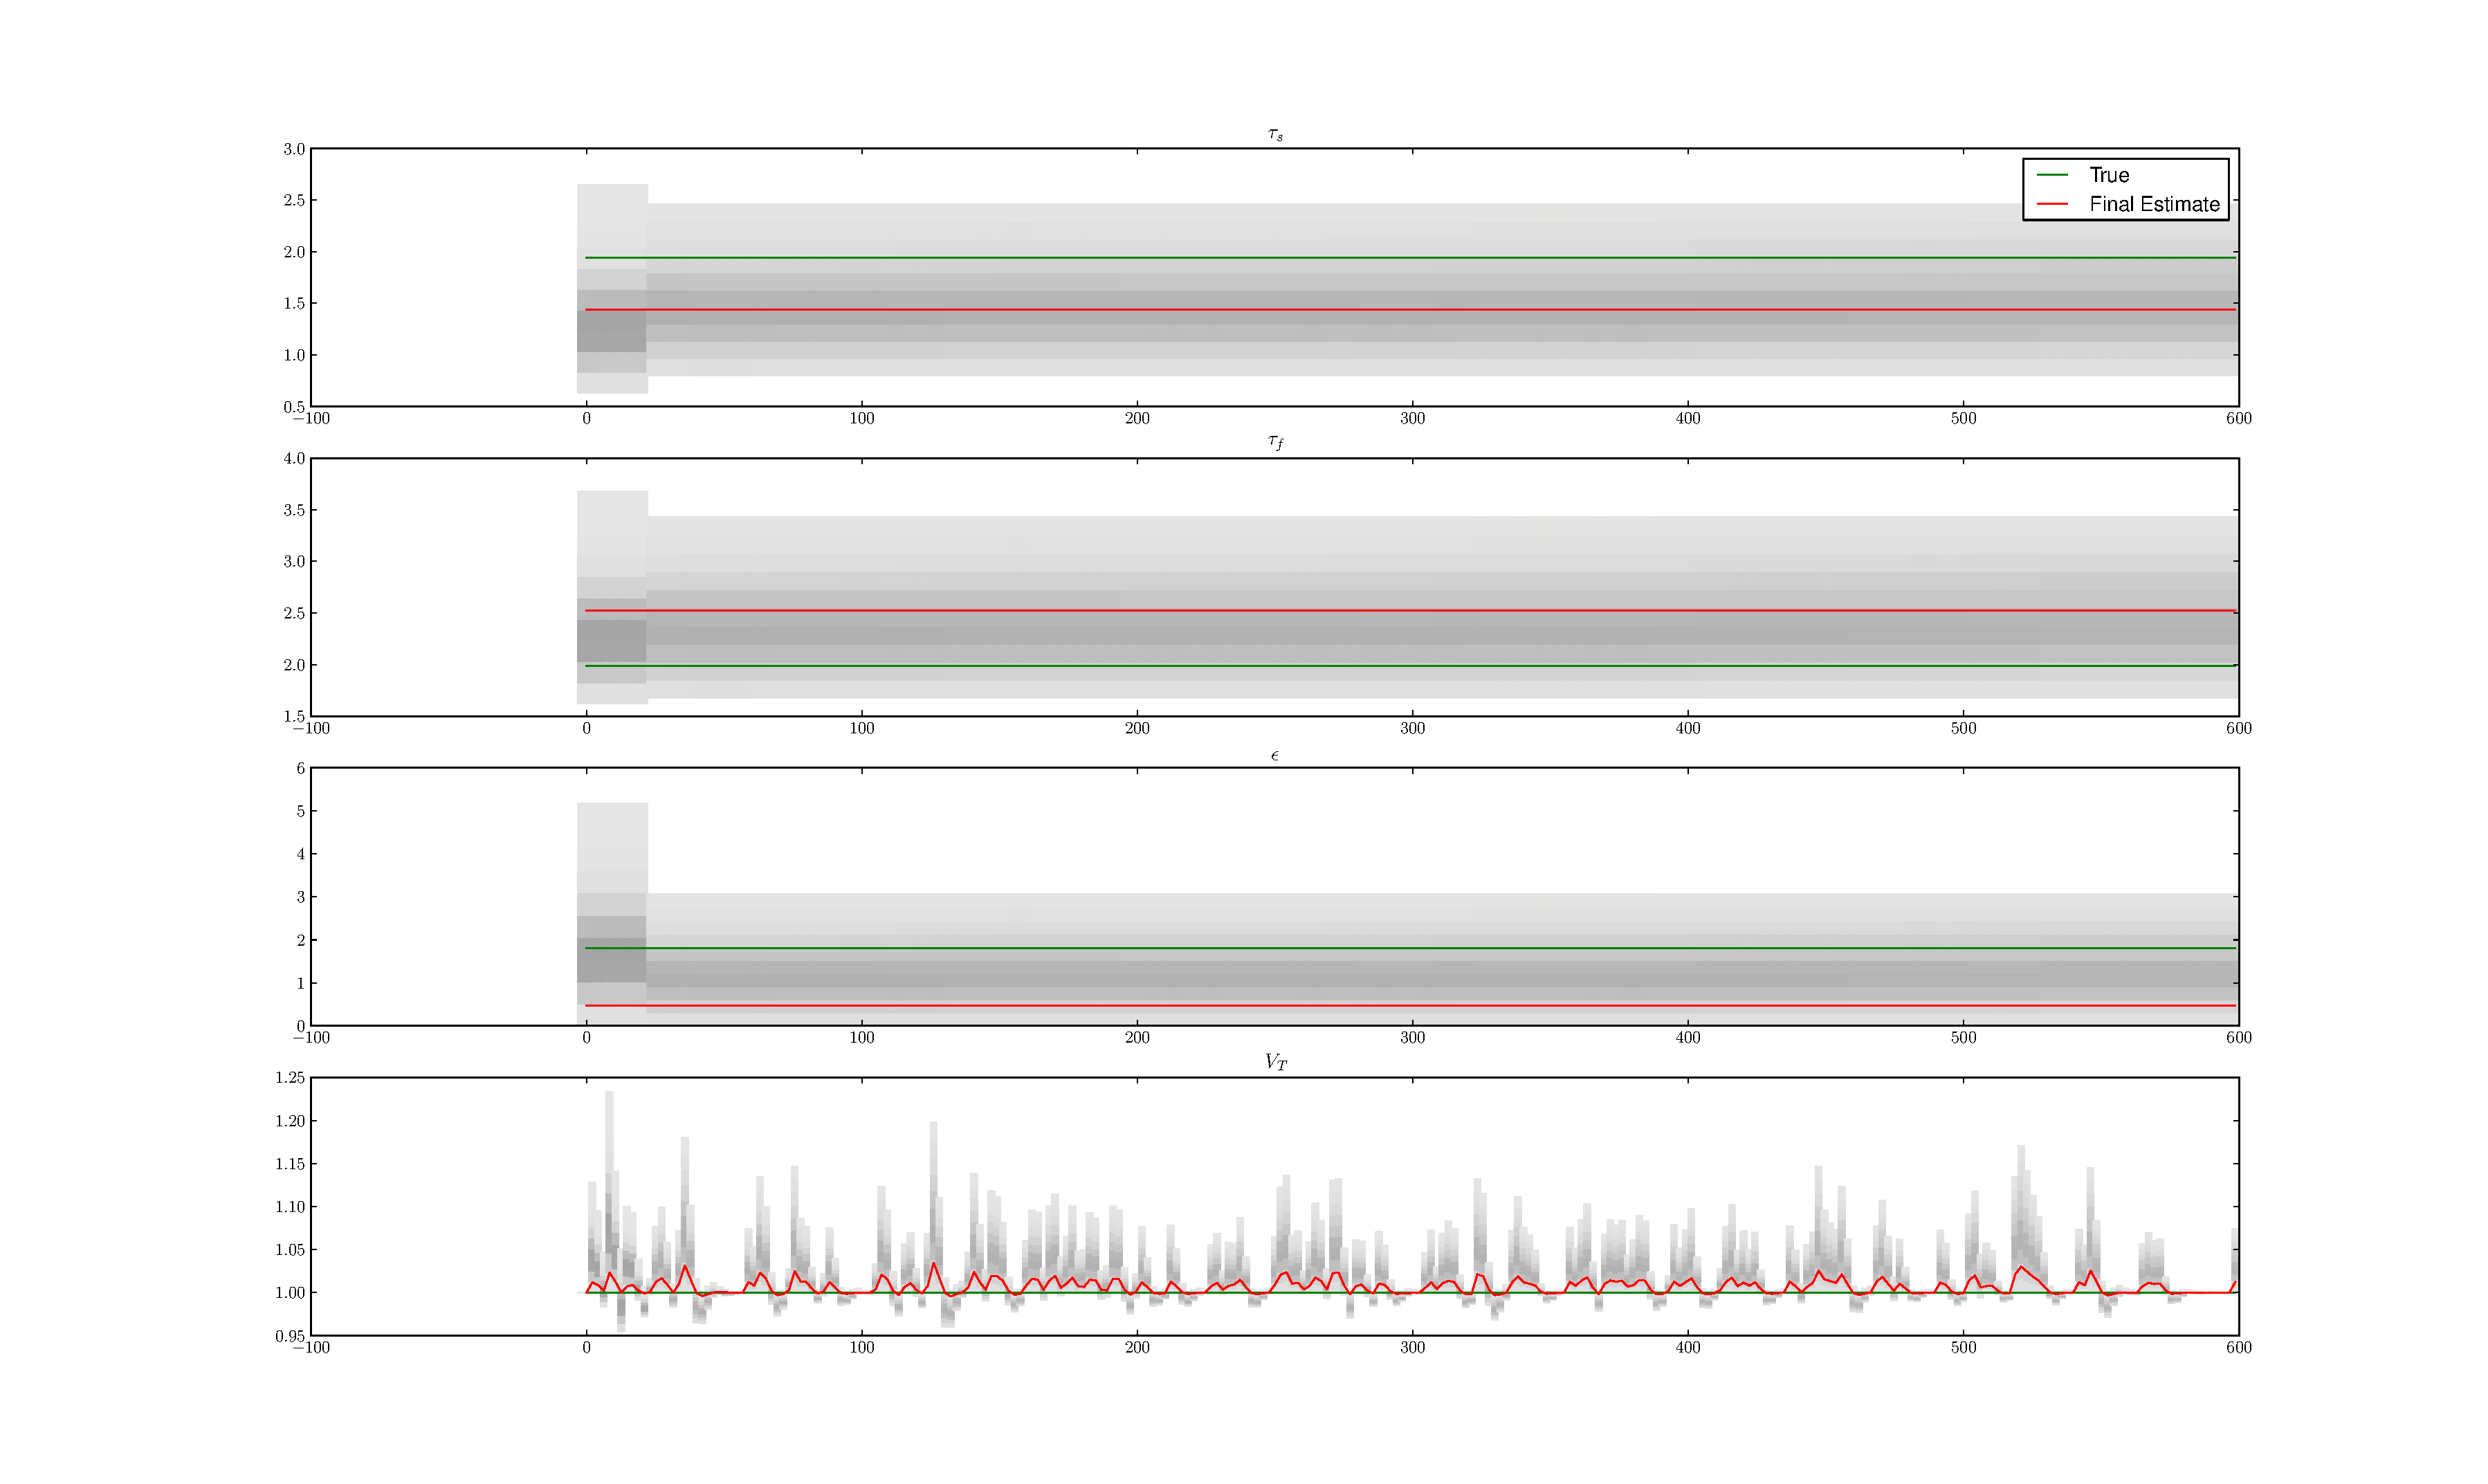
\includegraphics[clip=true,trim=6cm 2cm 6cm 3cm, height=9cm]{images/justnoise_hist_2}}\\
\end{figure}

\begin{figure}[H]
\centering
\subfigure[$Q$, $S$, $F$, $BOLD$ ]
{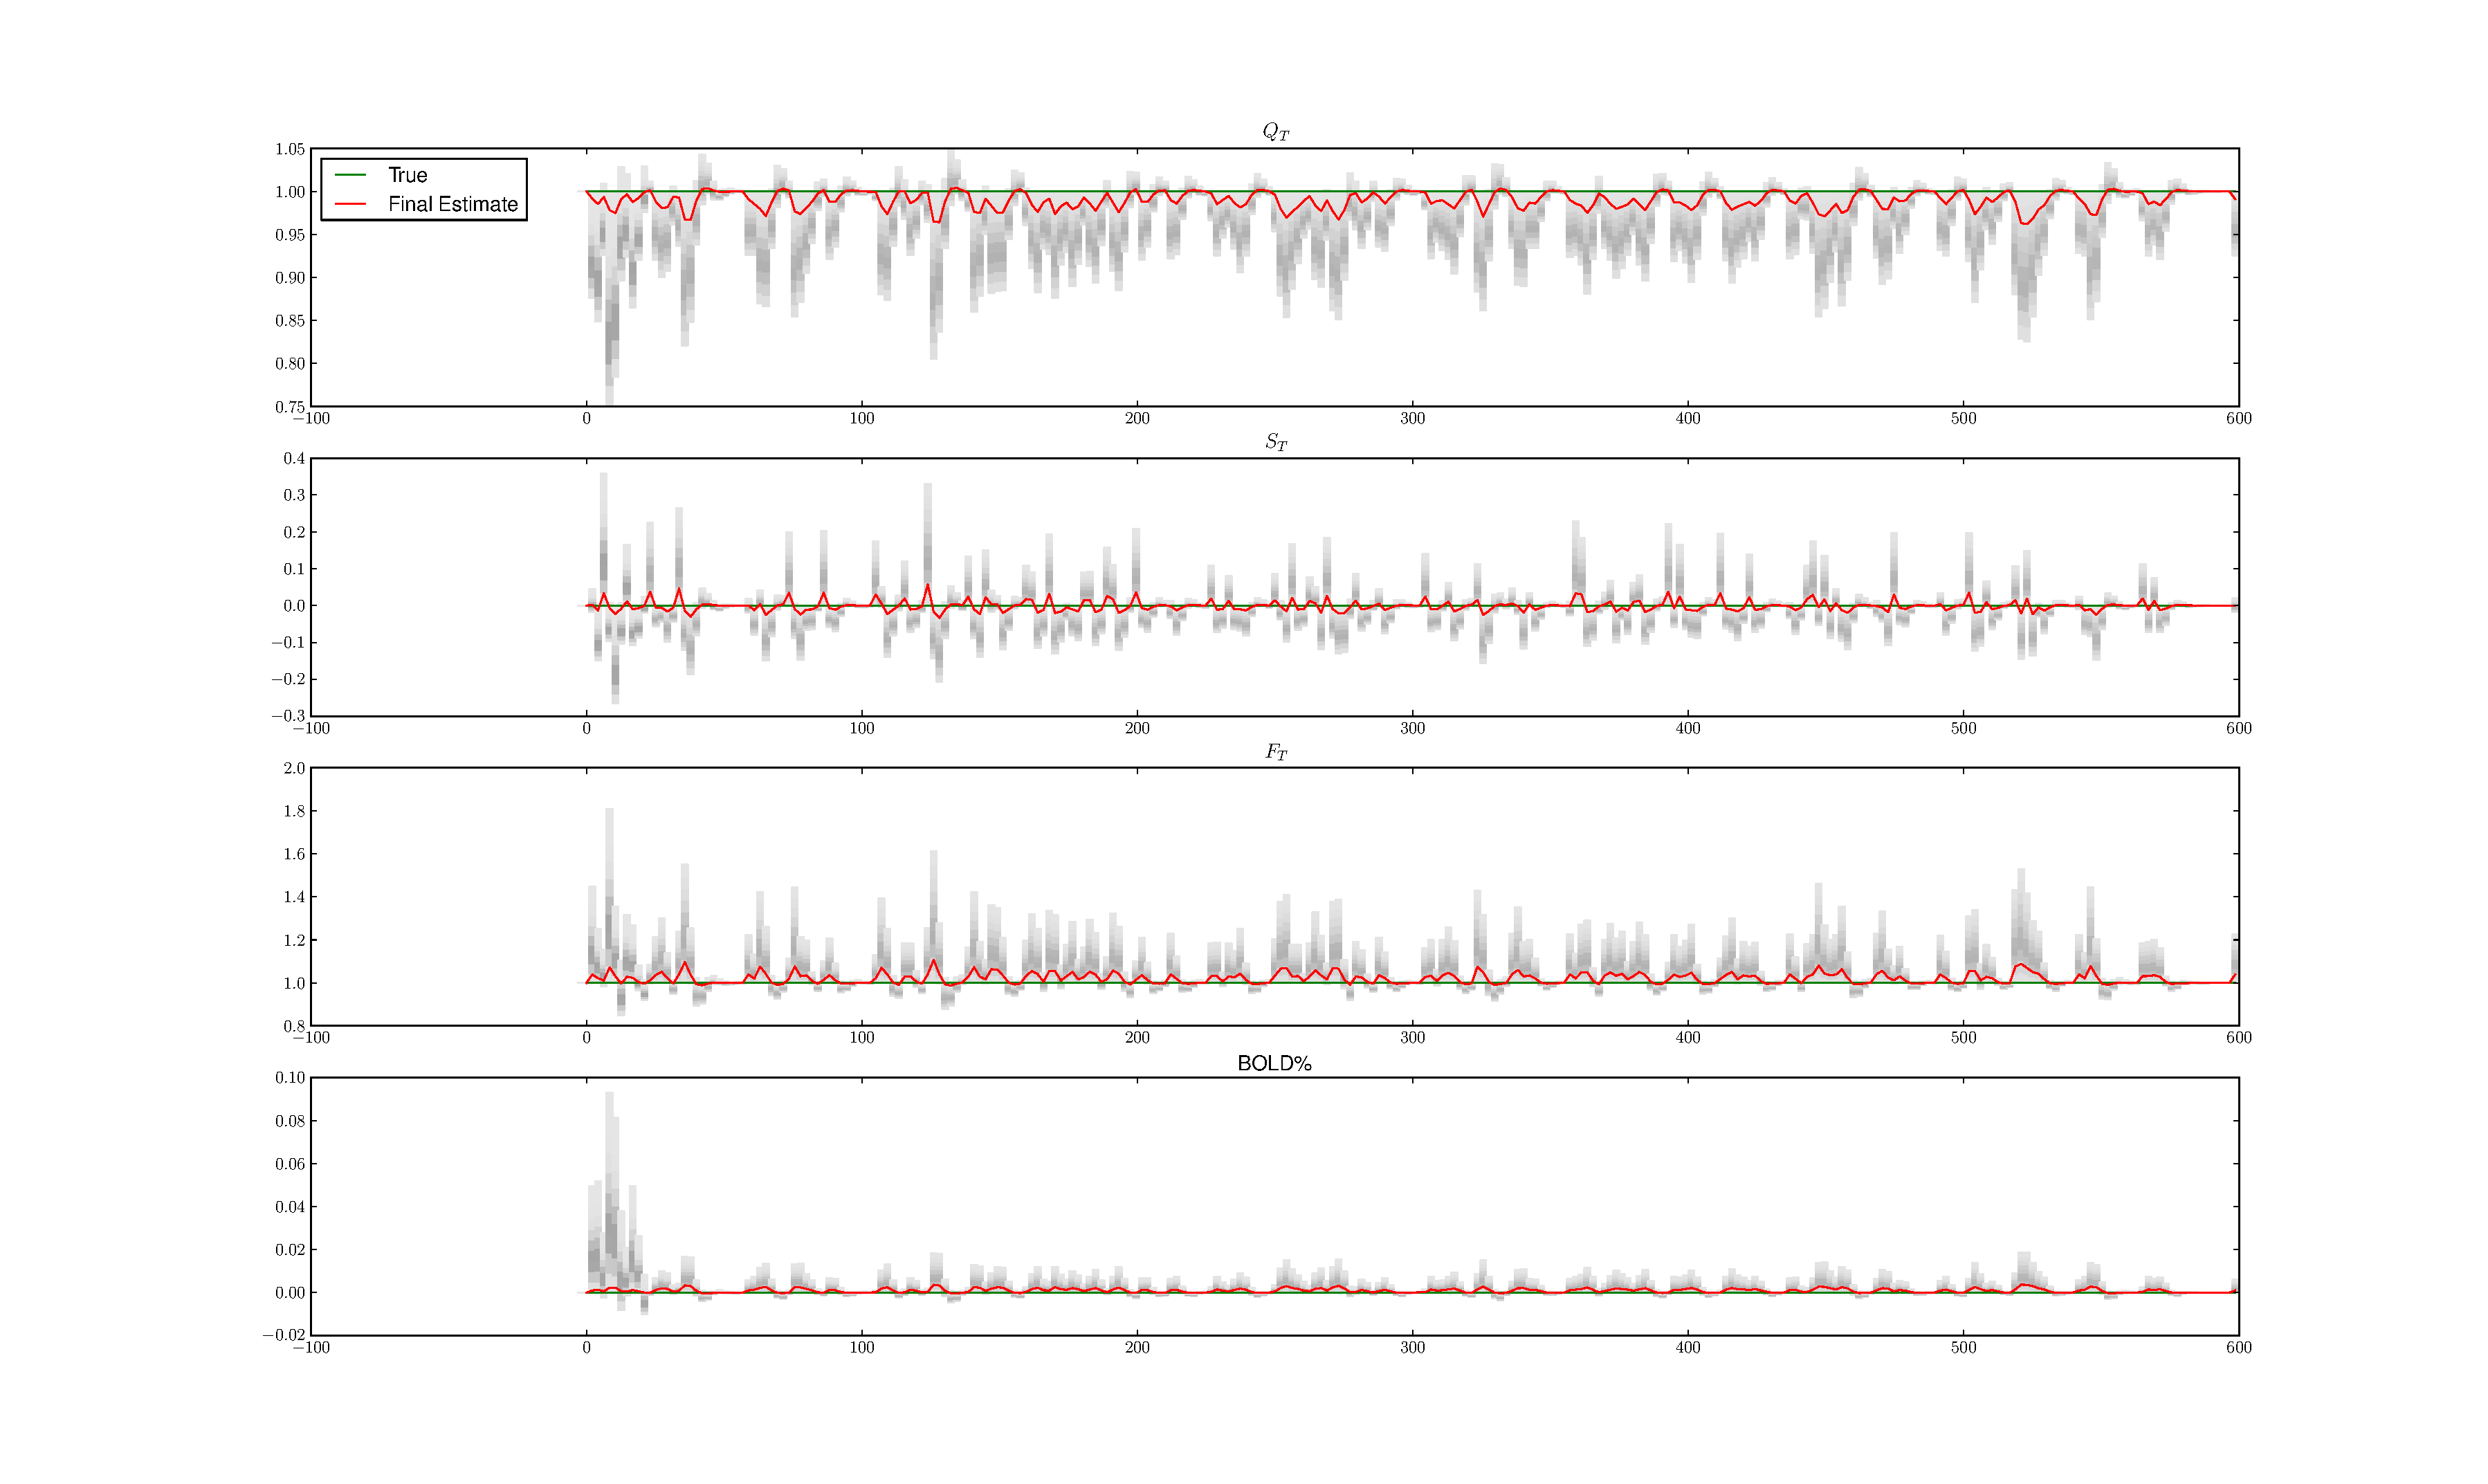
\includegraphics[clip=true,trim=6cm 2cm 6cm 3cm, height=9cm]{images/justnoise_hist_3}}
\caption{Converging histogram for parameters when the signal consists purely of low level noise. 
Same run as \autoref{fig:justnoise_fit_0}}
\label{fig:JustNoiseConvergence}
\end{figure}

From the results it is clear that the parameters have not taken any visible turns into
unrealistic territory. It appears individual parameters will not be a distinguishing factor
in determining the validity of the model. Additionally the raw square-root mean-squared-residual
also appears to be lower than the SMSR of the low noise simulation from earlier. 
The precision with which the convergence occurred is actually the best seen in any
simulation. 

However, the reason for low error may in fact be simply the fact that the over all
signal is significantly lower than any other simulation seen in other simulations.
The peaks never even cross 1\% difference, with most staying even below .5\% 
(\autoref{fig:PreprocessedNoiseOnly}). Because the signal is generally staying
well within the range of $.005$, which is the standard deviation of the weighting function
its unlikely that any particles will have a substantially different wieght. Thus, the reason
the fits are in such agreement is that no particles gained increased weight, and so
no convergence occurred at all, as further shown by \autoref{fig:JustNoiseConvergence}. 
Thus we have now seen how the particle filter responds when the signal is completely
random and low level, however there is also some possibility that the signal will
be random, yet active. Thus one more test is necessary on
a signal with enough noise to actually be considered a signal. 

%NO SIGNAL, VERY HIGH NOISE
\subsection{Pure Noise, High Magnitude}
\label{sec:PureNoiseHighMag}
To determine how the particle filter will respond to active, yet unrelated
portions of the brain, in this section random data will again be used, but
with even higher standard deviations. To simulate this case another
pure noise signal was generated using a $\sigma_x$ of $.1$ and a $\sigma_y$ of $.05$.

As before, the convergence all seems to follow a similar path, leaving almost no
variance in the estimated time series (\autoref{fig:fits_noiseonly_high}). Now, however
the peaks are comparable to peaks in a "real" timeseries. Interestingly the algorithm
suffered from almost constant particle deprevation, meaning that the heuristic
for rescuing the particle filter from particle deprivation, discuessed in
\autoref{sec:Resampling} in fact was working against the proper course of action. Of course
 the proper course of action in this case would be for the particle filter to fail,
 since no particle can really properly estimate a random sequence. When this mechanism
 was removed, all 11 runs stopped due to particle deprevation (all weights hit zero). 
 The problem with allowing particle deprivation to occur is that it can \emph{rarely}
 occur if the prior happens to not be dense enough in the area of the solution. Thus,
 there is an issue of false positives vs. false negatives. A middle ground, such as 
 allowing deprivation to occur if the recovery mechanism has already triggered once
 may be an acceptable compromise, however it would be difficult to strike the 
 right balance. Instead for the purposes here we depend on the square root MSR to 
 evaluate if the results were reasonable or not. 

\begin{figure}[H]
\centering
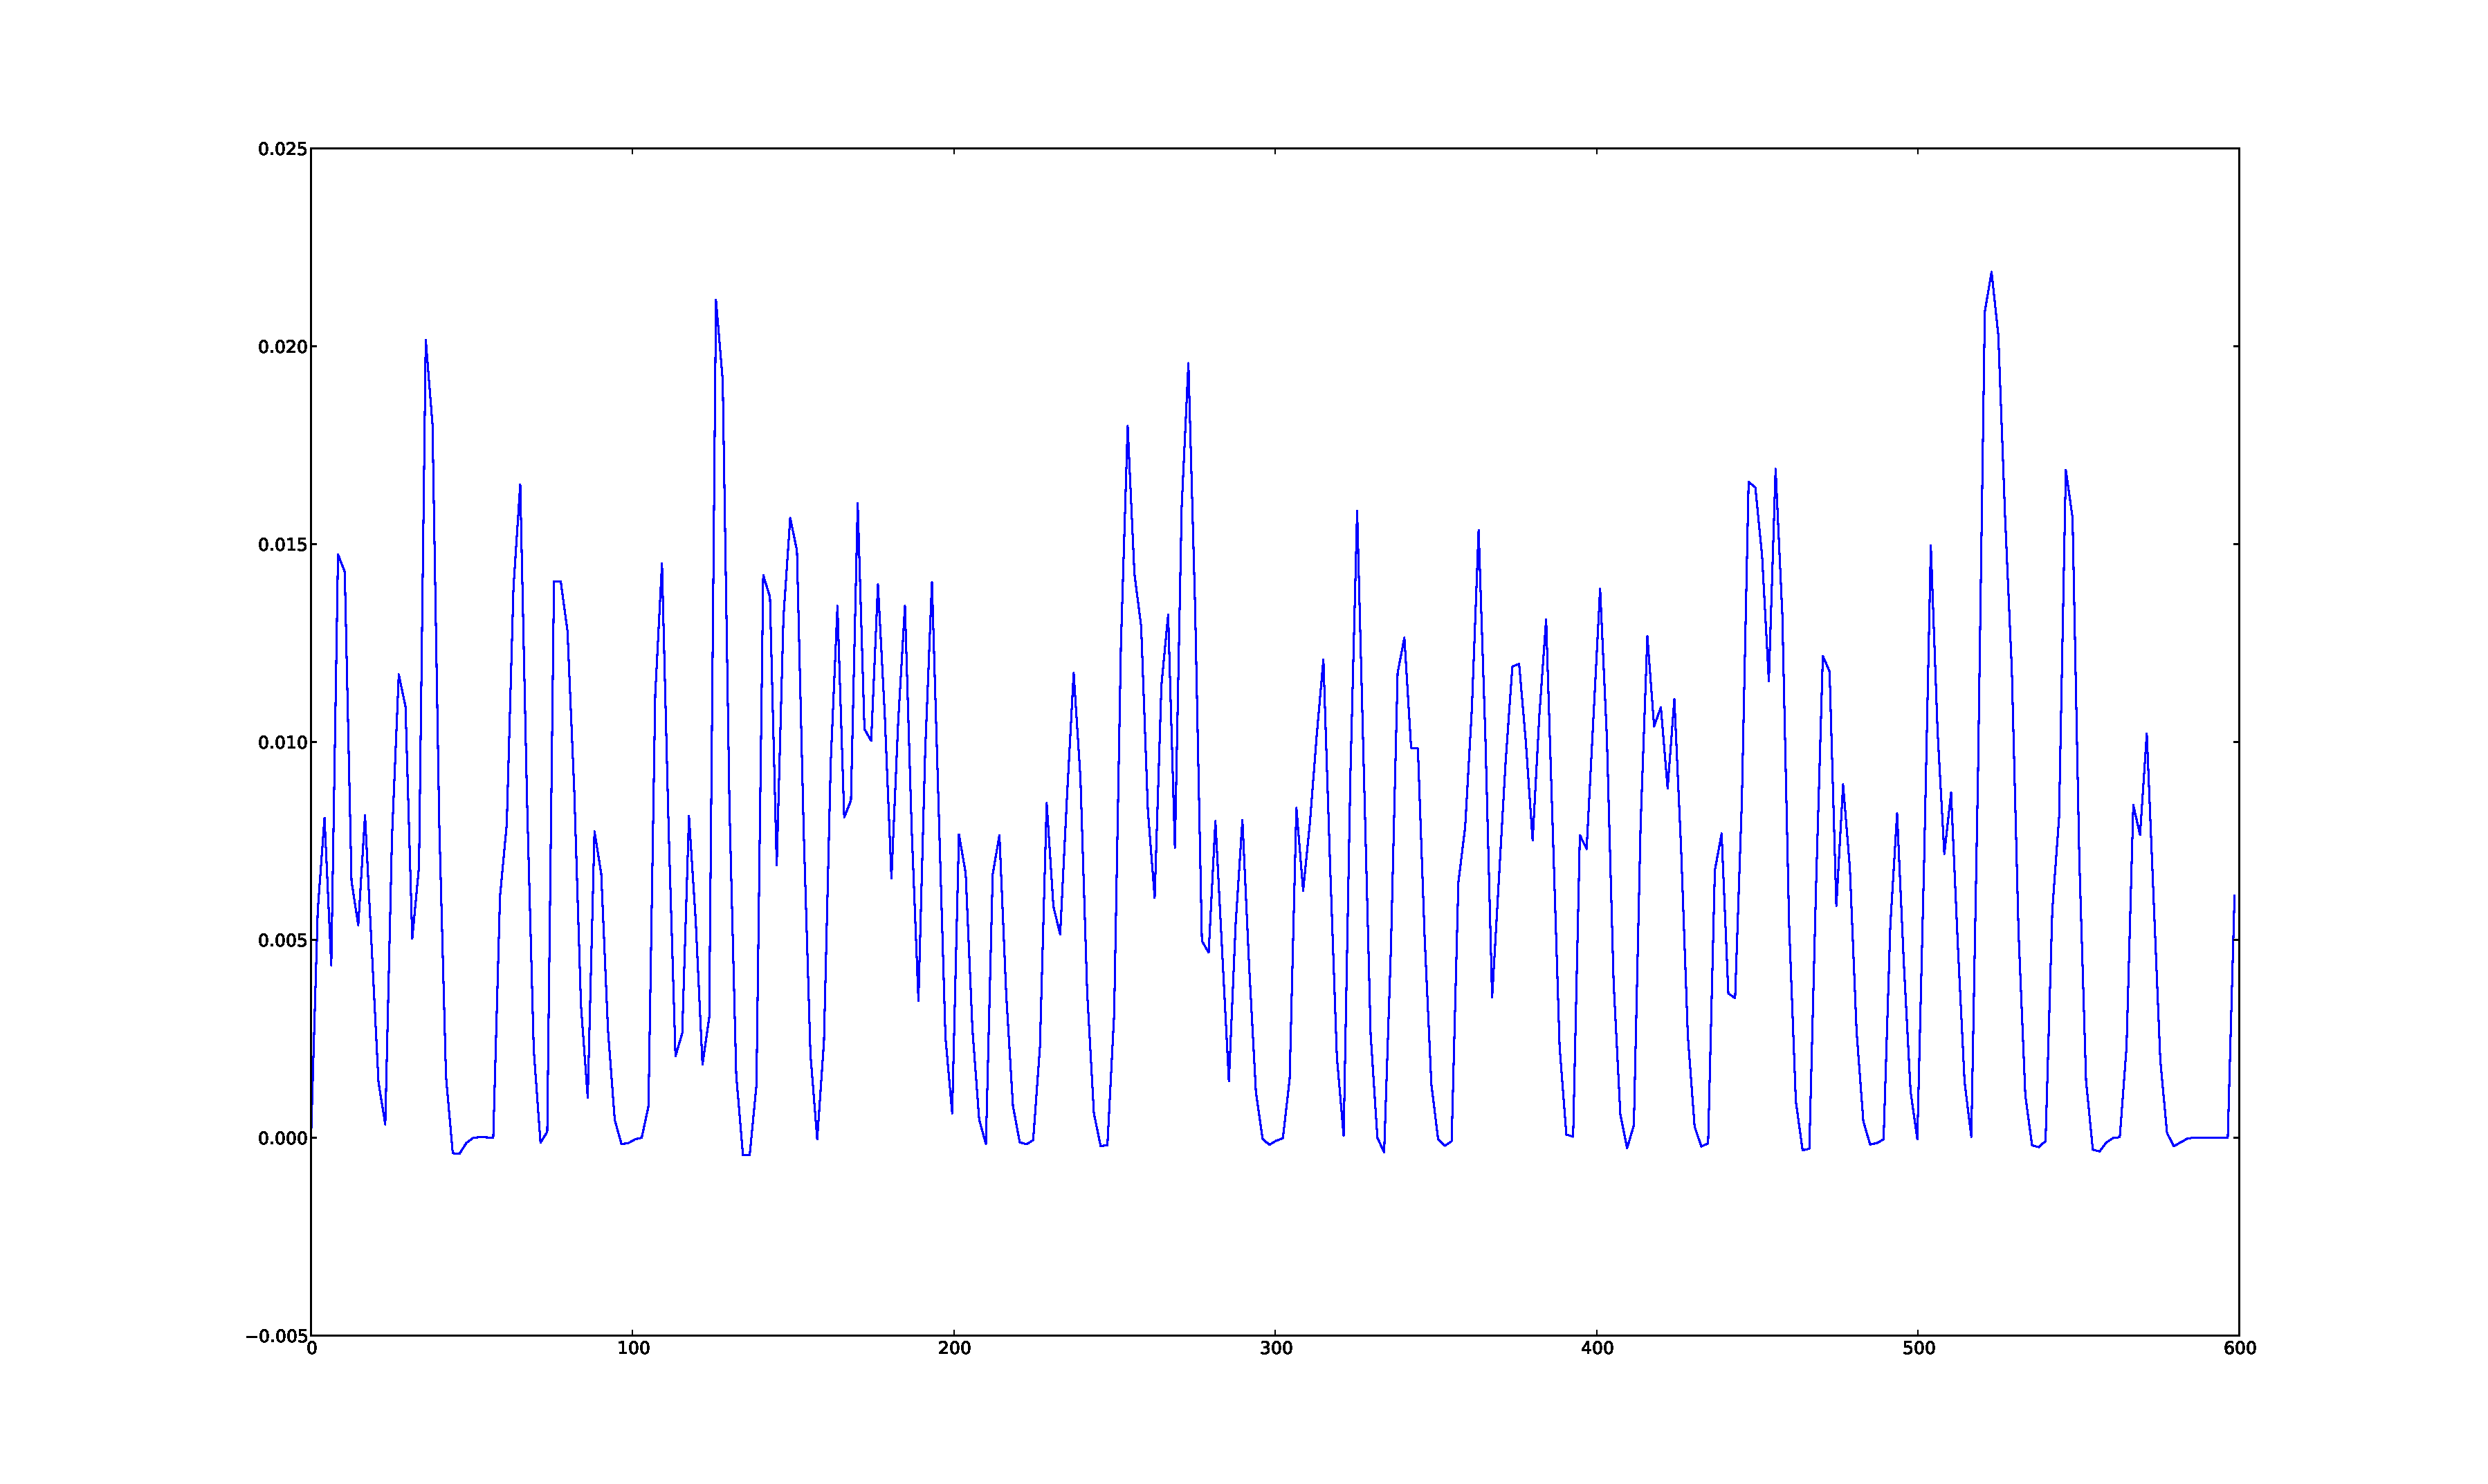
\includegraphics[clip=true,trim=6cm 3cm 6cm 3cm,height=9cm]{images/fits_noiseonly_high}
\caption{Fits to the non-active, high noise signal. Note that the line is thick because all
the fits overlap. This is all 11 fitted lines.}
\label{fig:fits_noiseonly_high}
\end{figure}

\begin{figure}[H]
\centering
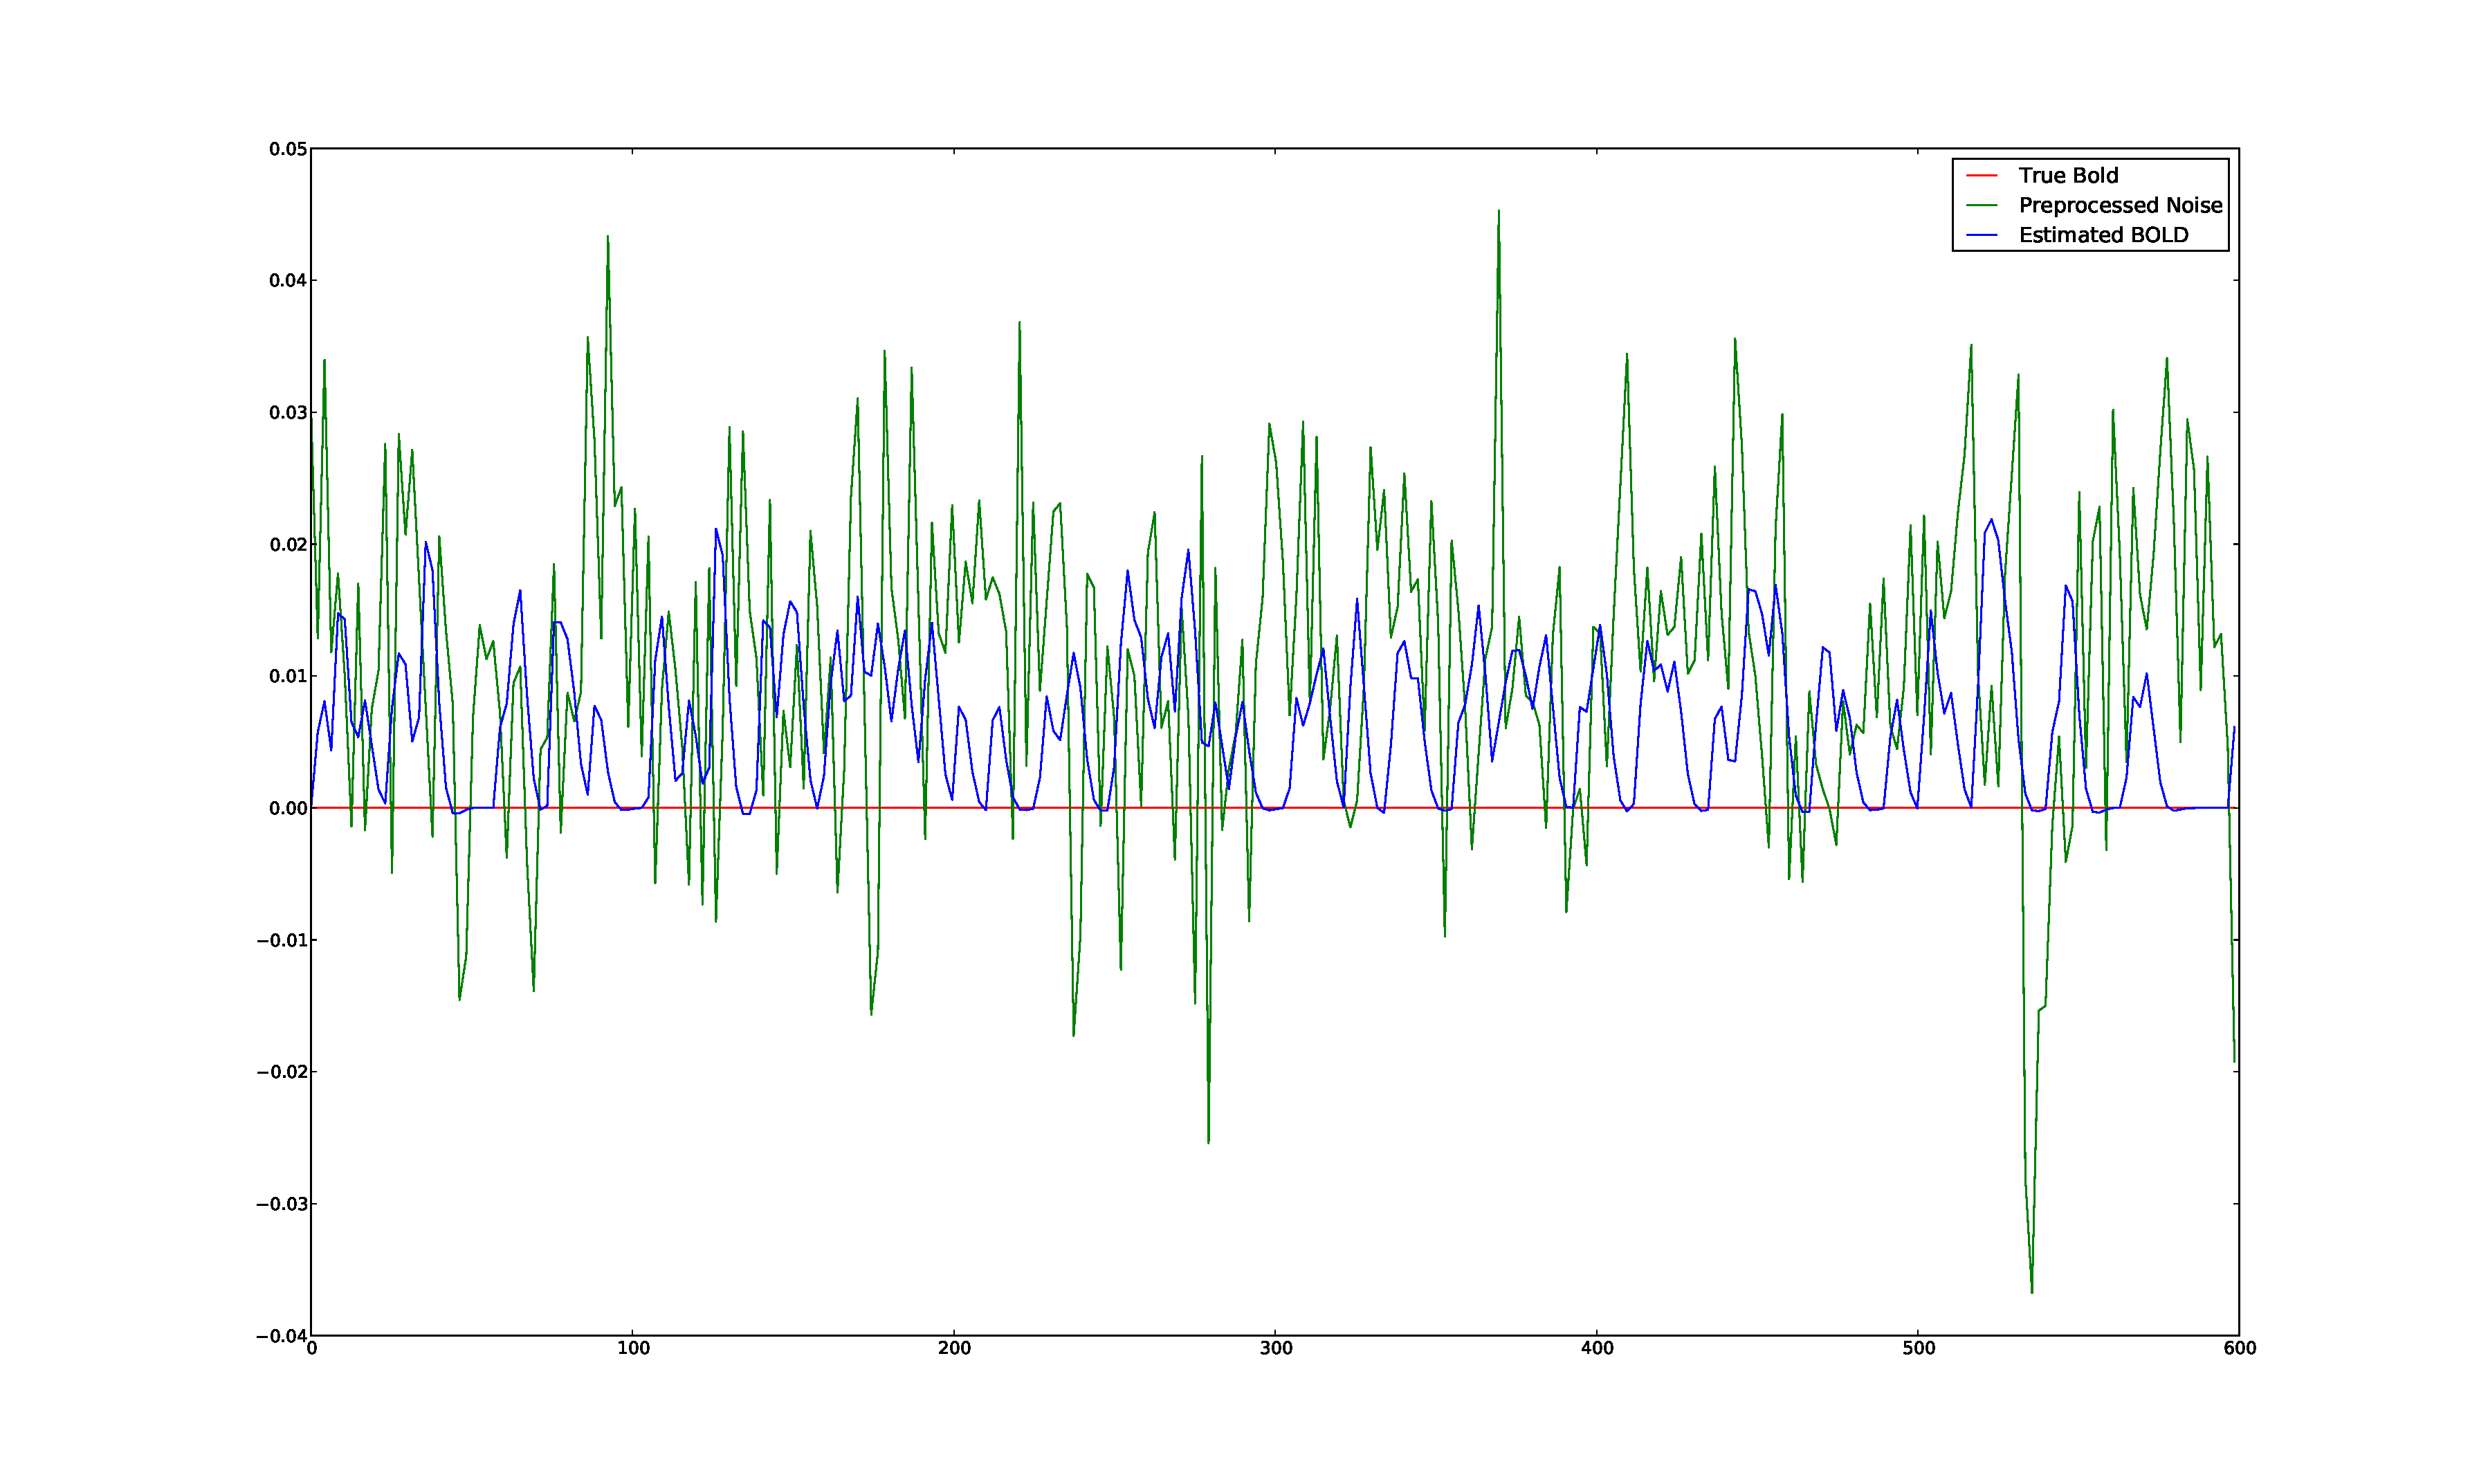
\includegraphics[clip=true,trim=6cm 3cm 6cm 3cm,height=9cm]{images/justbignoise_fit_0}
\caption{Fit from a single particle filter run, with the noise input. }
\label{fig:justbignoise_fit_0}
\end{figure} %uses allnoise/ALLNOISE-0-w0

\begin{figure}[H]
\centering
\subfigure[$\tau_0$, $\alpha$, $E_0$, $V_0$]
{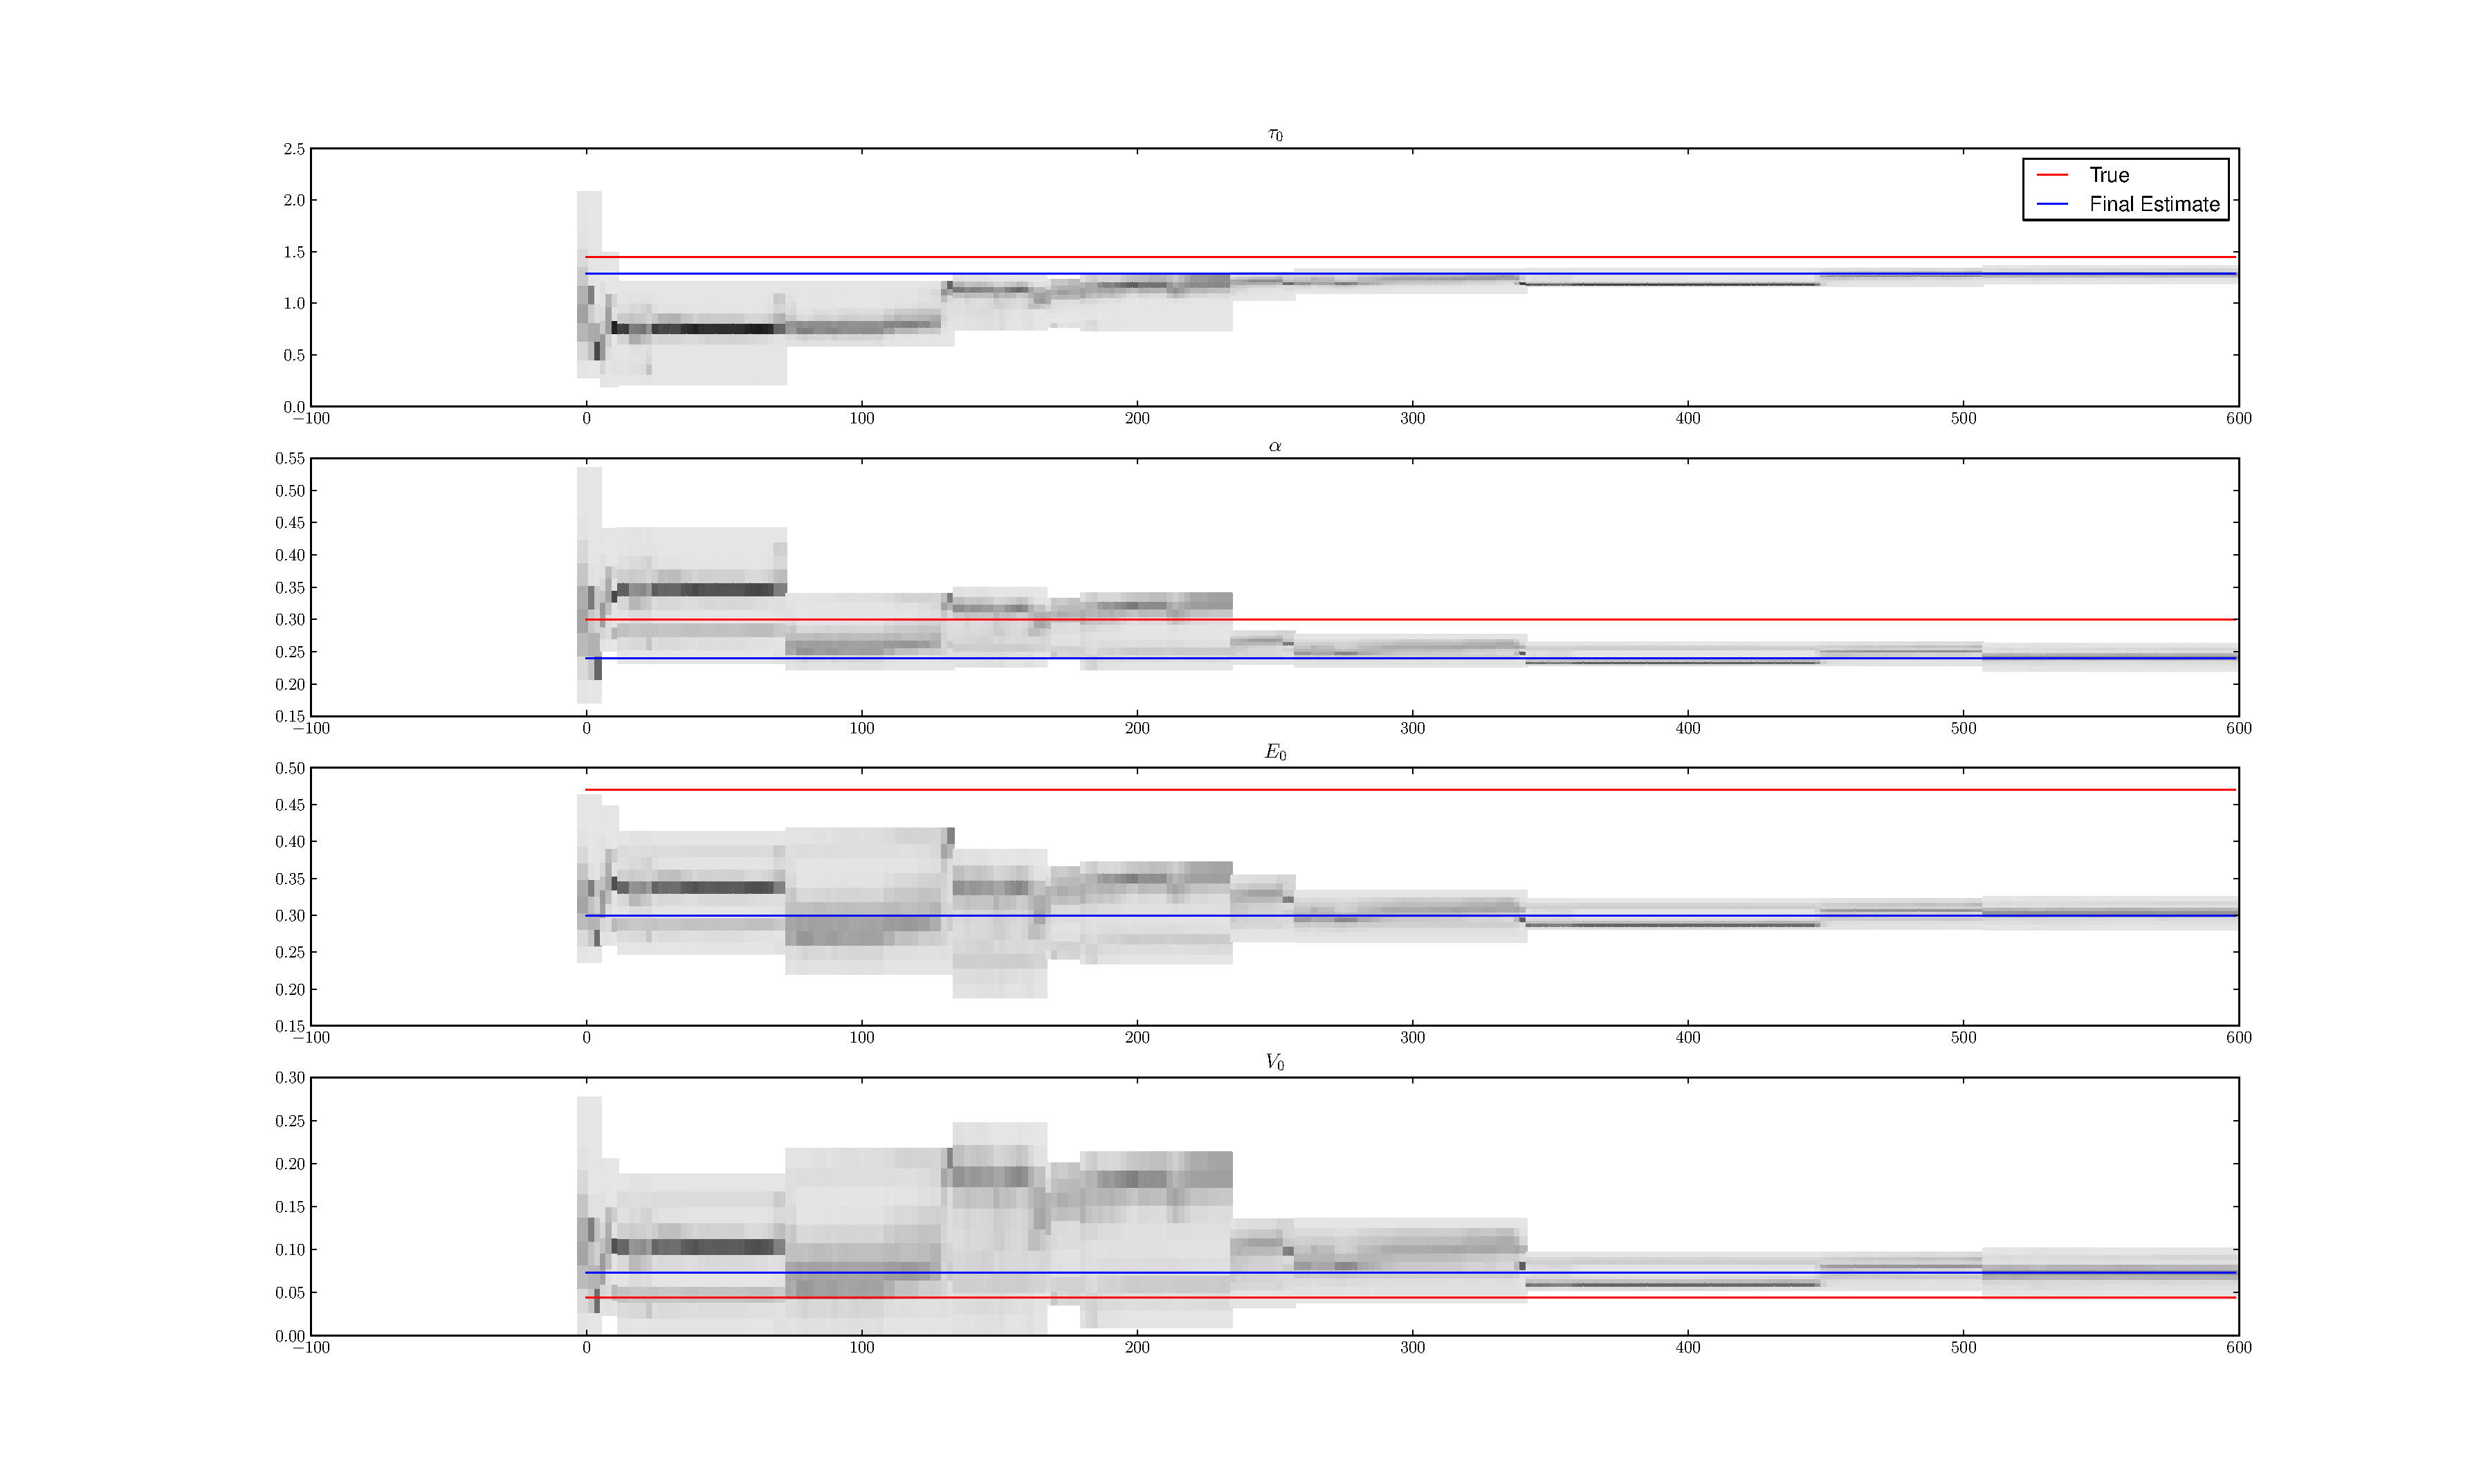
\includegraphics[clip=true,trim=6cm 3cm 6cm 3cm, height=9cm]{images/justbignoise_1}}\\
\end{figure}
\begin{figure}[H]
\subfigure[$\tau_s$, $\tau_f$, $\epsilon$, $V$] 
{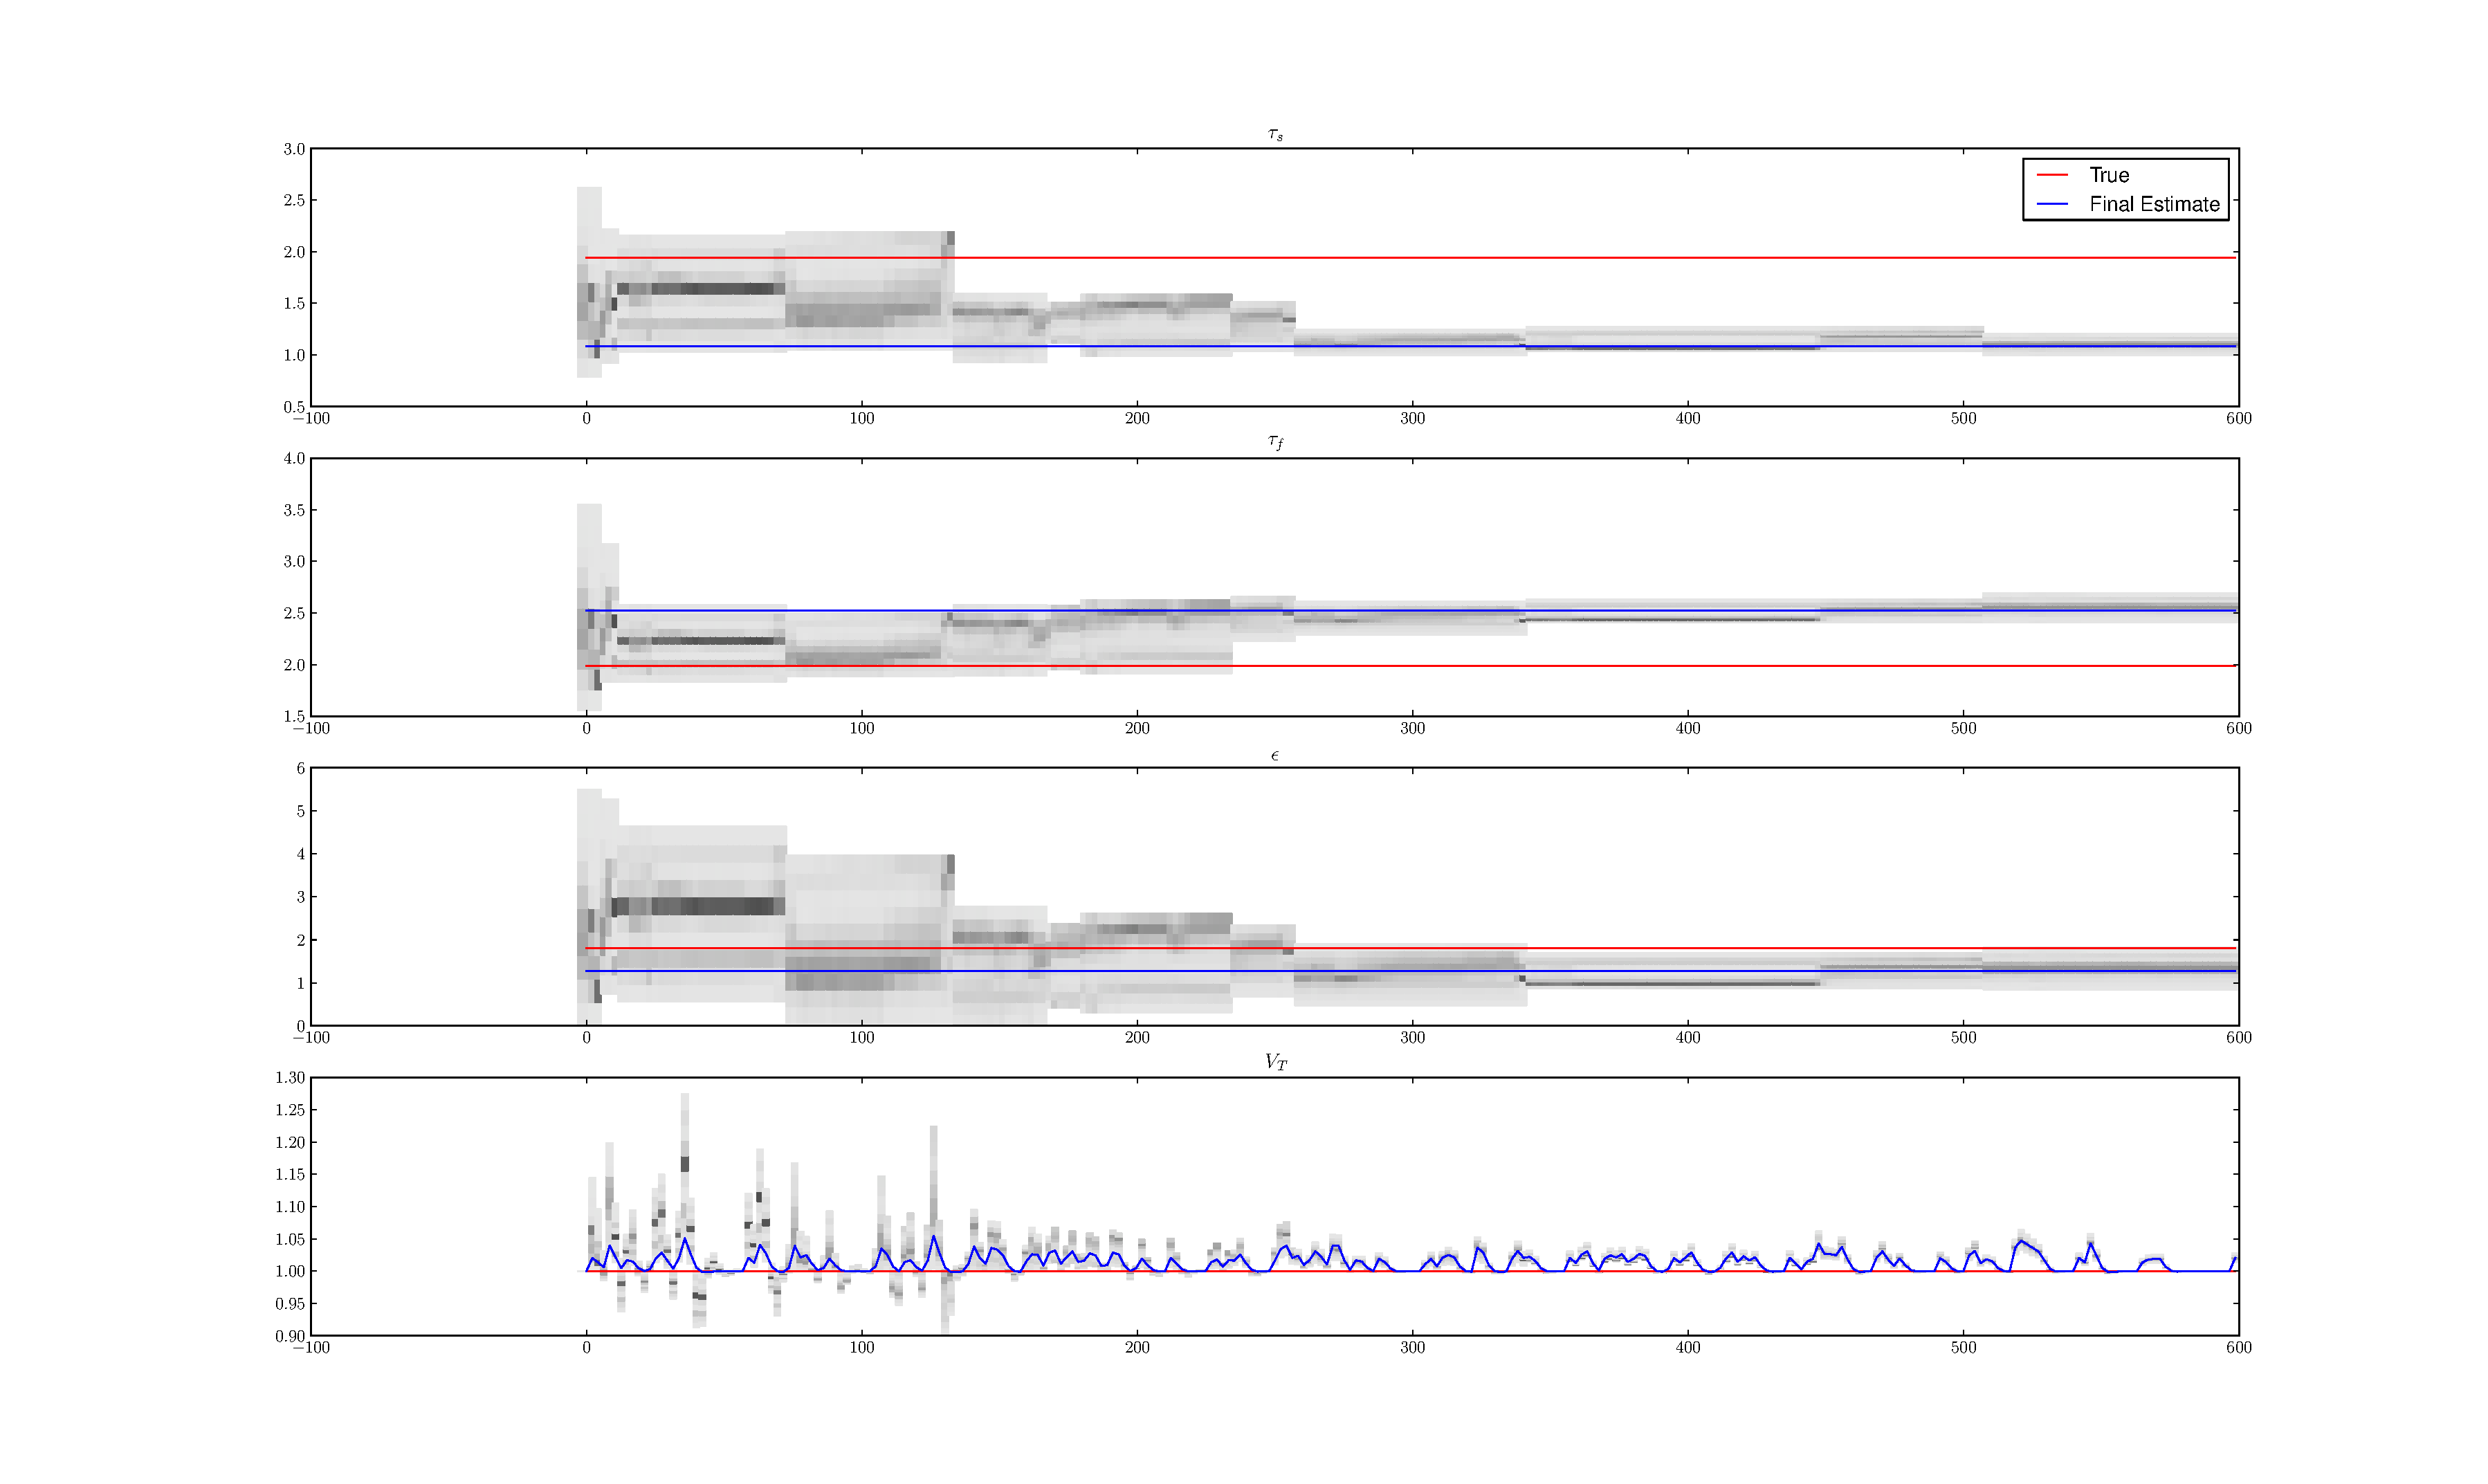
\includegraphics[clip=true,trim=6cm 3cm 6cm 3cm, height=9cm]{images/justbignoise_2}}\\
\end{figure}
\begin{figure}[H]
\subfigure[$Q$, $S$, $F$, $BOLD$ ]
{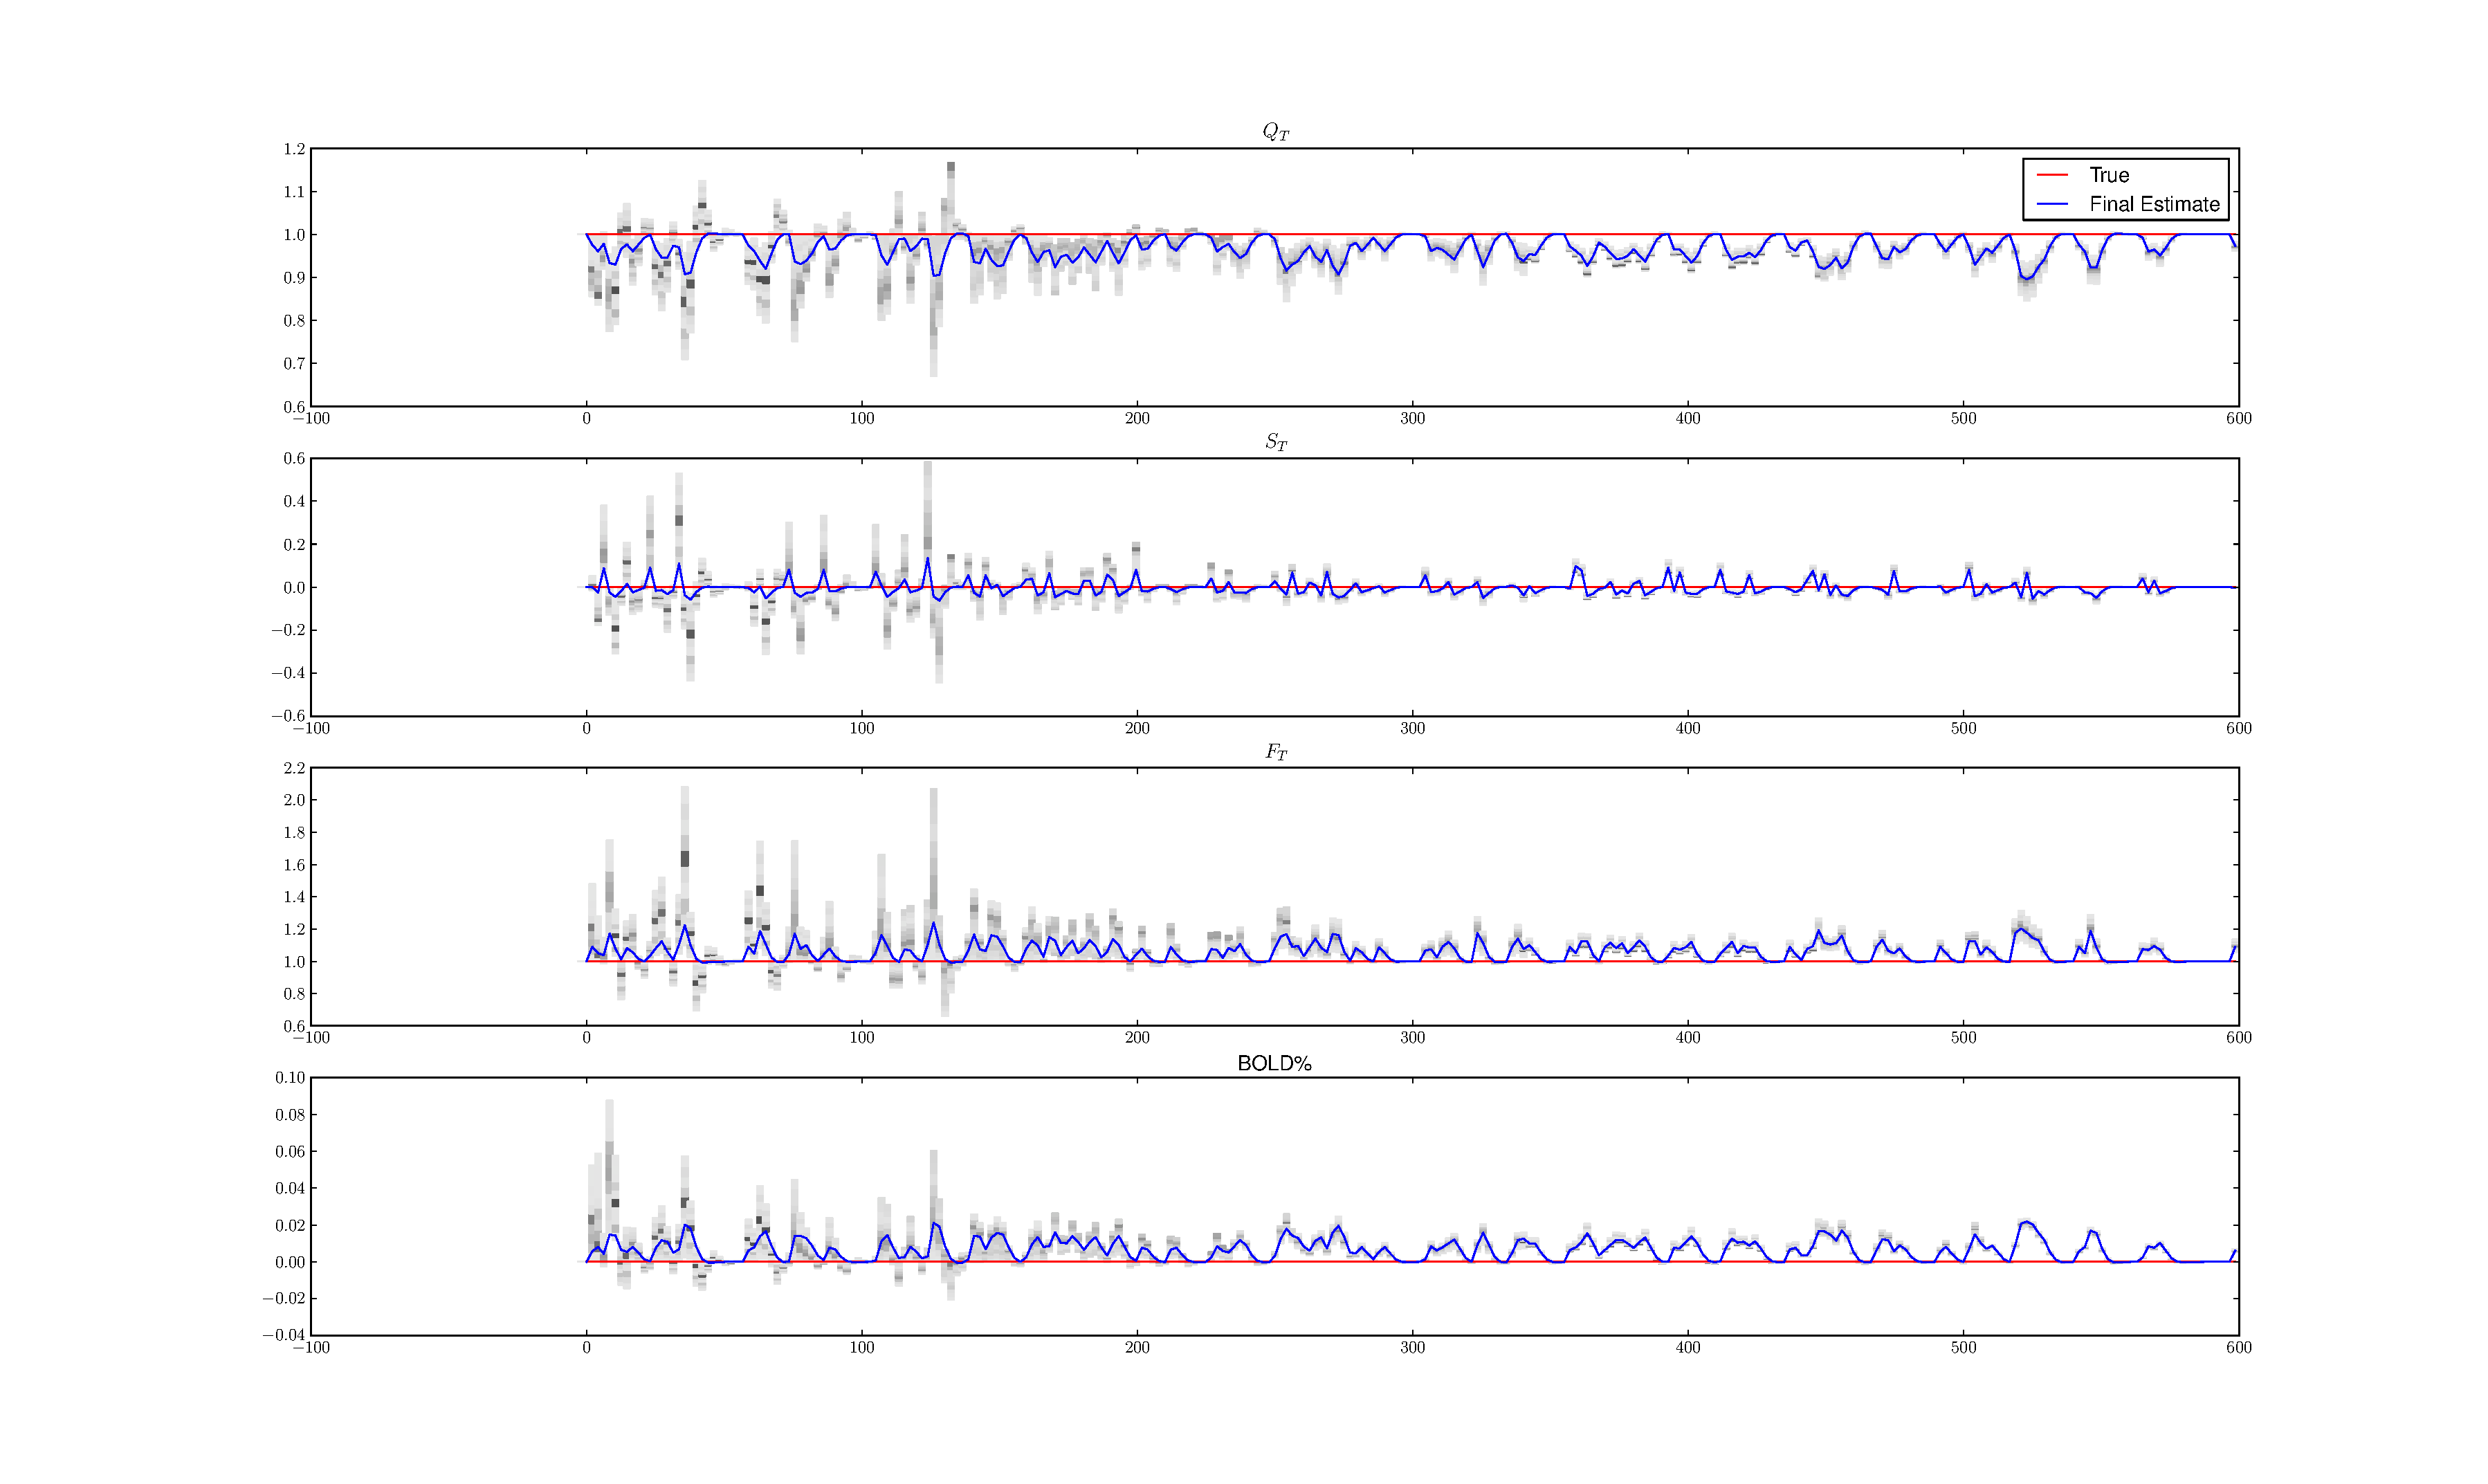
\includegraphics[clip=true,trim=6cm 3cm 6cm 3cm, height=9cm]{images/justbignoise_3}}
\caption{Converging histogram for parameters when the signal consists purely of noise, with peaks comparable  to 
the convential BOLD signal. ($\sigma_y = .01, \sigma_x = .005$). Same run as fit in \autoref{fig:justbignoise_fit_0}}
\label{fig:JustNoiseConvergenceLarge}
\end{figure}

From \autoref{fig:justbignoise_fit_0} it is clear that, despite the fact that the input 
is competely detached from the signal, a non-zero response by the particle filter does
lead to decreased MSR. This is primarily due to the preprocessing which forces the signal to
have a non-zero mean. While this scheme does create a type of artificial activation for
the particle filter, in reality the MSR will still be less than if the signal was left
with zero mean, and the particle filter stayed flat. At best the particle filter will 
over-smooth creating a line that does down the center of the noisy signal. In such a case
the MSR will be the same as the alternative. 

\subsection{Single Voxel Review}
\begin{table}[t]
\centering
\begin{tabular}{|c | c | c | c | c | c | c | c | c |}
\hline 
& \multicolumn{4}{|c|}{Signal} & \multicolumn{4}{|c|}{No Signal}\\
\hline
& \multicolumn{2}{|c|}{Low Noise} & \multicolumn{2}{|c|}{High Noise} 
& \multicolumn{2}{|c|}{$\sigma_y = .001, \sigma_x = .0005$} 
& \multicolumn{2}{|c|}{$\sigma_y = .01, \sigma_x = .005$}\\
\hline 
&$\sqrt{MSR}$ & $N\sqrt{MSR}$ &
 $\sqrt{MSR}$ & $N\sqrt{MSR}$ &
 $\sqrt{MSR}$ & $N\sqrt{MSR}$ &
 $\sqrt{MSR}$ & $N\sqrt{MSR}$ \\
\hline       
\hline       
1 & 0.003211 & 0.478015  & 0.014065  & 1.038941    &0.001667 & 1.295007 & 0.015114 & 1.33641 \\
2 & 0.003055 & 0.531771  & 0.013731  & 0.951648  &  0.001586 & 1.301750 & 0.015510 & 1.336667 \\
3 & 0.003289 & 0.545798  & 0.012754 &  0.995392  &  0.001651 & 1.26287 &  0.013957 & 1.159567 \\
4 & 0.002847 & 0.498237  & 0.016726  & 1.161286  &  0.001506 & 1.431959 & 0.013814 & 1.099876 \\
5 & 0.003006 & 0.468048  & 0.013698 &  1.039724   & 0.001515 & 1.256645 & 0.014350 & 1.201072 \\
6 & 0.002833 & 0.459001  & 0.011495 &  1.002143  &  0.001557 & 1.270797 & 0.013504 & 1.045886 \\
7 & 0.003028 & 0.460962  & 0.015550 &  1.088472   & 0.001585 & 1.154406 & 0.013006 & 1.205429 \\
8 & 0.003044 & 0.518376  & 0.012054 &  1.059620  &  0.001643 & 1.274564 & 0.015446 & 1.122502 \\
9 & 0.003345 & 0.525303  & 0.015104 &  1.015703  &  0.001679 & 1.320244 & 0.014847 & 1.086366 \\
10 & 0.003175 &0.492111  & 0.012493  & 1.189964  &  0.001826 & 1.344562 & 0.013125 & 1.221350 \\
11 & 0.002889 &0.490919  & 0.012165 &  0.953676  &  0.001950 & 1.325223 & 0.014457 & 1.117367 \\
\hline
mean & 0.003066 & 0.497140  & 0.013621 &  1.04514   &  0.001651 & 1.294366 & 0.014285 & 1.175681 \\
\hline
\end{tabular}
\caption{$\sqrt{MSE}$ and the normalized $\sqrt{MSE}$, 
    $\left(\sqrt{MSE}/(\text{Median Absolute Deviation})\right)$ for different configurations.} 
\label{tab:SignleVoxelActivationComparison} 
\end{table}

The first step in determining the validity of a model to provide and order of quality
to rate the results by. Unfortunately, because of the variablity in the signal levels the
raw $\sqrt{MSR}$ cannot perform this task. As demonstrated by \autoref{sec:PureNoiseLowMag},
just because the square-root mean-squared-residual is low doesn't mean the fit is
"good". Therefore, instead we will normalize the signal based on a value proportional to
the magnitude of the signal. Considering the tendency of FMRI noise to have large unexplainable
peaks and troughs, rather than using MAX and MIN values, I used a robust estimator of 
scale, the Median-Absolute-Deviation (MAD). Technically this is an estimator of the standard
deviation, however in this case it is also a good estimator of the scale of the input
signal. Thus, each point in the estimate as well as the original signal may be divided by
this, leading to a normalized signal. Instead, however, I simply divided the 
$\sqrt{MSR}$ by the MAD, which is functionally equivalent but leaves the  BOLD
levels intact for further analysis. The normalized square root MSR values are 
shown in \autoref{tab:SignleVoxelActivationComparison}. 

Comparing the results of \autoref{sec:HighNoise} and \autoref{sec:PureNoiseHighMag}, it is
clear that distinguishing between these cases is a difficult prospect. One possibility
is to just allow the particle filter to fail when particle deprivation occurs; however,
as discussed in the previous section, that could open the door to more false negatives.
Naturally there is a noise ceiling above which it will be impossible to determine model 
validity. The fact
that the particle filter is able to get close to the "true" signal is sadly irrelevant
when the noise is this high.
Ultimately, a threshold well below those shown in the high noise case 
will have to be placed on the error, if any confidence is going to be placed in
the results. Luckily the "high noise" case featured in \autoref{sec:HighNoise}
is actually noisier than typical FMRI.

\section{Multi-voxel Simulation}
To test the usefullness of the particle filter for Second I used a modified version of the FSL tool 
POSSUM to generate an entire FMRI image from a parameter map. The parameter map was generated
by taking an existing activation map and assigning discrete parameter sets to each region.
The result was a four dimensional (length x width
x height x parameter) image with spatially varying parameters. Possum was then modified
to take a parameter map and generate activation levels depending on the parameters at that
point. The patch for POSSUM will be made available. As an unfortunate side effect of 
not using Possums' original activation scale, I manually added 750 to the total level of
simulated Possum images. This is because the BOLD \% difference levels were in the range
of 50 - 100\% from the base, about 5 times as large as they should have been. Ultimately
this should not have an effect on the parameters (other than perhaps $\epsilon$ and $V_0$). 
For each time-series in the simulated FMRI image, the final \emph{static} parameters were saved
into a parameter map. This parameter map may then be compared to the map used to generate the 
simulated data; additionally a new simulation using the calculated parameters may also be 
generated to test the difference in activation levels between the real parameters and the
estimated ones. Since it is clear that the parameters are not fully orthogonal 
(\cite{Deneux2006}), its possible that two sets of parameters are functionally equivalent,
but have different parameters. This way, an absolute 
quantitative difference between the two parameter sets may be found.

